\documentclass[12pt,a3paper]{article}

%% ── Packages ──────────────────────────────────────────────────────────
\usepackage{amsmath,amssymb}
\usepackage{geometry}
\usepackage{enumitem}
\usepackage{titlesec}
\usepackage[hidelinks,colorlinks=true,linkcolor=blue!70!black]{hyperref}
\usepackage{xcolor}
\usepackage{fancyhdr}
\usepackage{tcolorbox}
\usepackage{multicol}
\usepackage{needspace}
\usepackage[strings]{underscore}
\usepackage{array,booktabs}
\usepackage{multirow}
\usepackage[table]{xcolor}
\usepackage{tikz}
\usepackage{listings}
\usepackage{makecell}
\usepackage{tabularx}
\usepackage{tikz}
\usepackage{chemfig}
\usepackage{subcaption} % For side-by-side layout
\usepackage{circuitikz}
\usepackage{longtable}

\tcbuselibrary{listings}
\usetikzlibrary{circuits.logic.US,calc}

\usetikzlibrary{shapes.geometric, positioning, arrows.meta, calc}
\tcbuselibrary{skins,breakable}
\geometry{margin=2.5cm,headheight=20pt,top=3cm,bottom=3cm}

%% ── Colors ────────────────────────────────────────────────────────────
\definecolor{pblue}{RGB}{13,71,161}
\definecolor{dgray}{RGB}{66,66,66}
\definecolor{cA}{RGB}{183,28,28}
\definecolor{cB}{RGB}{1,87,155}
\definecolor{cC}{RGB}{27,94,32}
\definecolor{cD}{RGB}{106,27,154}
\definecolor{cE}{RGB}{230,81,0}
\definecolor{cF}{RGB}{0,96,100}
\definecolor{cG}{RGB}{136,14,79}
\definecolor{cH}{RGB}{0,77,64}
\definecolor{cI}{RGB}{62,39,35}

\definecolor{pbbblue}{HTML}{005CC5}
\definecolor{pcomment}{HTML}{6A737D}
\definecolor{pstring}{HTML}{032F62}
\definecolor{glassybg}{RGB}{245,246,250}

%% ── Code listing style ────────────────────────────────────────────────
\lstdefinestyle{Cstyle}{
  language=C,
  basicstyle=\small\ttfamily,
  keywordstyle=\bfseries\color{pbbblue},
  commentstyle=\itshape\color{pcomment},
  stringstyle=\color{pstring},
  numberstyle=\tiny\color{gray},
  numbers=left,
  stepnumber=1,
  numbersep=10pt,
  breaklines=true,
  frame=l,
  framesep=4.5mm,
  framexleftmargin=2.5mm,
  rulecolor=\color{pblue!50},
  backgroundcolor=\color{glassybg},
  fillcolor=\color{white},
  aboveskip=15pt,
  belowskip=15pt,
  showstringspaces=false,
  tabsize=4
}
\lstset{style=Cstyle}

%% ── Section headings ──────────────────────────────────────────────────
\titleformat{\section}{\large\bfseries\color{pblue}}{}{0em}{}[\titlerule]
\titleformat{\subsection}{\normalsize\bfseries}{}{0em}{}

%% ── Header / Footer ───────────────────────────────────────────────────
\pagestyle{fancy}\fancyhf{}
\renewcommand{\headrulewidth}{0.5pt}
\fancyhead[L]{\small\textcolor{pblue}{\textbf{BUET $|$ CSE 103 Question Bank}}}
\fancyhead[R]{\small\textcolor{dgray}{\textit{\nouppercase{\leftmark}}}}
\fancyfoot[C]{\small\thepage}

%% ── Utility macros ────────────────────────────────────────────────────
\newcommand{\yr}[1]{\hfill\textcolor{gray}{\small\textbf{[#1]}}}
\newcommand{\mk}[1]{\textcolor{orange!70!black}{\small\textbf{(#1 marks)}}}
\newcommand{\variant}[1]{\par\vspace{1pt}\textcolor{blue!50!black}%
  {\footnotesize\textit{$\hookrightarrow$ Similar: #1}}}
\newcommand{\visualnote}[1]{\par\vspace{2pt}%
  {\footnotesize\textcolor{cG}{\textit{\textbf{[Visual:} #1\textbf{]}}}}}

%% ── Subtopic heading macro ────────────────────────────────────────────
\newcommand{\subtopic}[2]{%
  \vspace{10pt}
  \noindent\begin{tcolorbox}[colback=#1!8,colframe=#1,boxrule=0.6pt,arc=4pt,
    left=6pt,right=6pt,top=4pt,bottom=4pt]
    \small\bfseries\textcolor{#1}{#2}
  \end{tcolorbox}
  \vspace{2pt}
}

%% ── Section divider page ──────────────────────────────────────────────
\newcommand{\secdivider}[4]{%
  \newpage\thispagestyle{empty}%
  \vspace*{\fill}%
  \begin{tcolorbox}[enhanced,colback=#4!7,colframe=#3,boxrule=1.5pt,arc=8pt,
    left=20pt,right=20pt,top=22pt,bottom=22pt,
    shadow={3pt}{-3pt}{0pt}{black!15}]
    \centering
    {\large\textcolor{gray}{\textbf{BUET $\cdot$ CSE 103 $\cdot$ Discrete Mathematics}}}\\[8pt]
    {\fontsize{26}{32}\selectfont\bfseries\textcolor{#3}{#1}}\\[6pt]
    {\fontsize{15}{19}\selectfont\textcolor{dgray}{#2}}\\[12pt]
    \textcolor{#3!60}{\rule{0.5\textwidth}{0.5pt}}\\[6pt]
    {\small\textcolor{gray}{#2}}
  \end{tcolorbox}%
  \vspace*{\fill}\newpage%
}

%% ── List styles ───────────────────────────────────────────────────────
\setlist[enumerate,1]{label=\textbf{Q\arabic*.},leftmargin=*,itemsep=14pt,parsep=2pt}
\setlist[enumerate,2]{label=(\alph*),leftmargin=2em,itemsep=3pt}
\setlist[enumerate,3]{label=(\roman*),leftmargin=2.5em,itemsep=2pt}

\begin{document}

%% ══════════════════════════════════════════════════════════════════════
%%  COVER PAGE
%% ══════════════════════════════════════════════════════════════════════
\thispagestyle{empty}
\begin{tcolorbox}[enhanced,colback=pblue!5,colframe=pblue,boxrule=1.5pt,arc=6pt,
  top=28pt,bottom=28pt,left=22pt,right=22pt,
  shadow={4pt}{-4pt}{0pt}{black!20}]
  \centering

  
\includegraphics[height=2.5cm]{images/buet_logo.png}\\[8pt]

  {\Large\bfseries\textcolor{pblue}{Bangladesh University of Engineering and Technology}}\\[4pt]
  {\normalsize\textcolor{dgray}{Department of Computer Science \& Engineering}}\\[18pt]
  \textcolor{pblue}{\rule{\textwidth}{1pt}}\\[14pt]
  {\fontsize{22}{28}\selectfont\bfseries\textcolor{pblue}{Discrete Mathematics Question Bank}}\\[8pt]
  {\fontsize{14}{18}\selectfont\textcolor{dgray}{CSE 103 $\cdot$ Discrete Mathematics}}\\[4pt]
  \textcolor{pblue}{\rule{\textwidth}{0.5pt}}\\[14pt]
  {\small\textcolor{dgray}{Year Coverage: 2006--07 to 2024--25\\Topics:\;Mathematical Logic, Proof Techniques, Set Theory \& Functions,\\
  Relations \& Partial Orders, Number Theory \& Algebra,\\
  Counting \& Combinatorics, Recurrence Relations, Graph Theory,\\
  Trees, Discrete Probability}}\\[16pt]
  
    {\small\bfseries\textcolor{dgray}{Authors \& Contributors}}\\[6pt]
    \begin{tabular}{rl}
      \textcolor{dgray}{\textbf{Md Ratul Hasan}} \textcolor{dgray}{\small(2405009)}
        & --- Question Curation \& Organisation\\
       \textcolor{dgray}{\textbf{Ibtasam Haider Riddho}} \textcolor{dgray}{\small(2505009)} & --- \LaTeX\ Typesetting\\[3pt]
       \textbf{NotebookLM} & --- Research \& Extraction\\[3pt]
       \textbf{Claude AI} & --- \LaTeX\ Typesetting \& Formatting\\
      \textbf{Gemini} & --- Diagram Generation\\[3pt]
    \end{tabular}
\end{tcolorbox}
\newpage

%% ══════════════════════════════════════════════════════════════════════
%%  TABLE OF CONTENTS
%% ══════════════════════════════════════════════════════════════════════
\thispagestyle{fancy}\markboth{Table of Contents}{}
\begin{center}
  {\LARGE\bfseries\textcolor{pblue}{Table of Contents}}\\[6pt]
  \textcolor{pblue}{\rule{0.6\textwidth}{0.8pt}}
\end{center}
\vspace{6pt}

%% Part I
\begin{tcolorbox}[breakable,colback=cA!5,colframe=cA,boxrule=1pt,arc=5pt,
  left=8pt,right=8pt,top=8pt,bottom=8pt,before skip=4pt]
  {\large\bfseries\textcolor{cA}{Part I --- Logic \& Proof Techniques}}\\[5pt]
  \textcolor{cA!40}{\rule{\textwidth}{0.4pt}}\\[3pt]
  \small\begin{itemize}[leftmargin=1.2em,itemsep=1pt,label={\textcolor{cA}{$\triangleright$}}]
    \item \hyperref[sec:S1]{\textbf{S1.} Mathematical Logic}
      \begin{itemize}[leftmargin=1.5em,itemsep=0pt,label={\textcolor{cA}{$\cdot$}}]
        \item \hyperref[sub:s1-proplogic]{Propositional Logic}
        \item \hyperref[sub:s1-predlogic]{Predicate Logic}
        \item \hyperref[sub:s1-proplogic-inference]{Arguments \& Rules of Inference}
        \item \hyperref[sub:s1-reasoning]{Mathematical Reasoning}
      \end{itemize}
    \item \hyperref[sec:S2]{\textbf{S2.} Proof Techniques}
      \begin{itemize}[leftmargin=1.5em,itemsep=0pt,label={\textcolor{cA}{$\cdot$}}]
        \item \hyperref[sub:s2-direct]{Direct Proof \& Counterexamples}
        \item \hyperref[sub:s2-contrapositive]{Proof by Contrapositive \& Indirect Proofs}
        \item \hyperref[sub:s2-contradiction]{Proof by Contradiction \& Existence Proofs}
        \item \hyperref[sub:s2-induction]{Mathematical Induction}
      \end{itemize}
  \end{itemize}
\end{tcolorbox}

%% Part II
\begin{tcolorbox}[breakable,colback=cB!5,colframe=cB,boxrule=1pt,arc=5pt,
  left=8pt,right=8pt,top=8pt,bottom=8pt,before skip=4pt]
  {\large\bfseries\textcolor{cB}{Part II --- Set Theory \& Relations}}\\[5pt]
  \textcolor{cB!40}{\rule{\textwidth}{0.4pt}}\\[3pt]
  \small\begin{itemize}[leftmargin=1.2em,itemsep=1pt,label={\textcolor{cB}{$\triangleright$}}]
    \item \hyperref[sec:S3]{\textbf{S3.} Set Theory}
      \begin{itemize}[leftmargin=1.5em,itemsep=0pt,label={\textcolor{cB}{$\cdot$}}]
        \item \hyperref[sub:s3-sets]{Sets}
        \item \hyperref[sub:s3-functions]{Functions}
        \item \hyperref[sub:s3-sum]{Summations}
        \item \hyperref[sub:s3-paradox]{Paradox}
      \end{itemize}
    \item \hyperref[sec:S4]{\textbf{S4.} Relations}
      \begin{itemize}[leftmargin=1.5em,itemsep=0pt,label={\textcolor{cB}{$\cdot$}}]
        \item \hyperref[sub:s4-relations]{Binary Relations}
        \item \hyperref[sub:s4-equivalence]{Equivalence Relations}
        \item \hyperref[sub:s4-poset]{Partial Ordered Sets}
        \item \hyperref[sub:s4-hasse]{Hasse diagram}
      \end{itemize}
  \end{itemize}
\end{tcolorbox}

%% Part III
\begin{tcolorbox}[breakable,colback=cC!5,colframe=cC,boxrule=1pt,arc=5pt,
  left=8pt,right=8pt,top=8pt,bottom=8pt,before skip=4pt]
  {\large\bfseries\textcolor{cC}{Part III --- Number Theory \& Counting}}\\[5pt]
  \textcolor{cC!40}{\rule{\textwidth}{0.4pt}}\\[3pt]
  \small\begin{itemize}[leftmargin=1.2em,itemsep=1pt,label={\textcolor{cC}{$\triangleright$}}]
    \item \hyperref[sec:S5]{\textbf{S5.} Number Theory \& Algebra}
      \begin{itemize}[leftmargin=1.5em,itemsep=0pt,label={\textcolor{cC}{$\cdot$}}]
        \item \hyperref[sub:s5-divisibility]{Divisibility \& Prime Numbers}
        \item \hyperref[sub:s5-gcdlcm]{GCD, LCM \& Linear Combinations}
        \item \hyperref[sub:s5-algebraic]{Algebraic Structures}
        \item \hyperref[sub:s5-modular]{Modular Arithmetic}
        \item \hyperref[sub:s5-cryptograpy]{Cryptography}
      \end{itemize}
    \item \hyperref[sec:S6]{\textbf{S6.} Counting \& Combinatorics}
      \begin{itemize}[leftmargin=1.5em,itemsep=0pt,label={\textcolor{cC}{$\cdot$}}]
        \item \hyperref[sub:s6-counting]{Counting Principles \& Foundations}
        \item \hyperref[sub:s6-combinations]{Combinations, Permutations \& Stars-and-Bars}
        \item \hyperref[sub:s6-pigeonhole]{Pigeonhole Principle \& Derangements}
        \item \hyperref[sub:s11-inclusion]{Inclusion-Exclusion Principle}
      \end{itemize}
  \end{itemize}
\end{tcolorbox}

%% Part IV
\begin{tcolorbox}[breakable,colback=cD!5,colframe=cD,boxrule=1pt,arc=5pt,
  left=8pt,right=8pt,top=8pt,bottom=8pt,before skip=4pt]
  {\large\bfseries\textcolor{cD}{Part IV --- Recurrences \& Probability}}\\[5pt]
  \textcolor{cD!40}{\rule{\textwidth}{0.4pt}}\\[3pt]
  \small\begin{itemize}[leftmargin=1.2em,itemsep=1pt,label={\textcolor{cD}{$\triangleright$}}]
    \item \hyperref[sec:S7]{\textbf{S7.} Recurrence Relations}
      \begin{itemize}[leftmargin=1.5em,itemsep=0pt,label={\textcolor{cD}{$\cdot$}}]
        \item \hyperref[sub:s7-recurrence-formulation]{Formulation \& Applications}
        \item \hyperref[sub:s7-recurrence-solving]{Solution Methods \& Theorems}
        \item \hyperref[sub:s7-genfunc]{Generating Functions}
      \end{itemize}
    \item \hyperref[sec:S8]{\textbf{S8.} Discrete Probability}
      \begin{itemize}[leftmargin=1.5em,itemsep=0pt,label={\textcolor{cD}{$\cdot$}}]
        \item \hyperref[sub:s8-basicprob]{Basic Probability \& Counting Principles}
        \item \hyperref[sub:s8-conditional]{Conditional Probability, Bayes' Theorem \& Trees}
      \end{itemize}
  \end{itemize}
\end{tcolorbox}

%% Part V
\begin{tcolorbox}[breakable,colback=cE!5,colframe=cE,boxrule=1pt,arc=5pt,
  left=8pt,right=8pt,top=8pt,bottom=8pt,before skip=4pt]
  {\large\bfseries\textcolor{cE}{Part V --- Graph Theory}}\\[5pt]
  \textcolor{cE!40}{\rule{\textwidth}{0.4pt}}\\[3pt]
  \small\begin{itemize}[leftmargin=1.2em,itemsep=1pt,label={\textcolor{cE}{$\triangleright$}}]
    \item \hyperref[sec:S9]{\textbf{S9.} Graph Theory}
      \begin{itemize}[leftmargin=1.5em,itemsep=0pt,label={\textcolor{cE}{$\cdot$}}]
        \item \hyperref[sub:s9-graphs]{Graphs \& Graph Properties}
        \item \hyperref[sub:s9-planargraphs]{Planar Graphs}
        \item \hyperref[sub:s9-isomorphism]{Graph Isomorphism}
        \item \hyperref[sub:s9-paths]{Paths, Euler \& Hamiltonian}
        \item \hyperref[sub:s9-traversal]{Graph Traversal}
        \item \hyperref[sub:s9-trees]{Trees}
      \end{itemize}
    \end{itemize}
\end{tcolorbox}

\newpage

%% ══════════════════════════════════════════════════════════════════════
%%  PART I — LOGIC & PROOF TECHNIQUES
%% ══════════════════════════════════════════════════════════════════════
\secdivider{Part I}{Logic \& Proof Techniques}{cA}{cA}

%% ── S1: Mathematical Logic ────────────────────────────────────────────
\section{S1 --- Mathematical Logic}
\label{sec:S1}
\markboth{S1 --- Mathematical Logic}{}

%%──────────────────────────────────────────────────────────────────────
\subtopic{cA}{Propositional Logic}
\label{sub:s1-proplogic}

\begin{enumerate}
  

\item The renowned detective Sherlock Holmes was called upon to unravel a most perplexing murder mystery. Sheldon was found dead, and Holmes gathered the following clues during his investigation:
\begin{enumerate}
    \item Sheldon, the murdered manufacturer, was killed by a blow to the head with a brass candlestick.
    \item Either Amy or Bernadette was in the dining room at the time of the murder.
    \item If Penny was in the kitchen at the time of the murder, then Howard killed Sheldon with a fatal dose of strychnine.
    \item If Amy was in the dining room at the time of the murder, then Leonard killed Sheldon.
    \item If Penny was not in the kitchen at the time of the murder, then Bernadette was not in the dining room when the murder was committed.
    \item If Bernadette was in the dining room at the time the murder was committed, then Raj killed Sheldon.
\end{enumerate}
Is it possible for the detective to derive the identity of the murderer from the above facts? If so, who murdered Sheldon? (Assume there was only one cause of death.)
\mk{15} \yr{CSE 103 | L-1/T-I | 2024--25}

%% 2008-09
\item The $n$-th statement in a list of 100 statements is ``Exactly $n$ of the statements in this list are false.''
\begin{enumerate}
  \item What conclusions can you draw from these statements?
  \item Answer part (i) if instead the $n$-th statement reads ``At least $n$ of the statements in this list are false.''
\end{enumerate}
\mk{8+8} \yr{CSE 103 | L-1/T-1 | 2023--24}

%% 2023-24
\item For each of the following sentences, determine whether an \textbf{inclusive or} or an \textbf{exclusive or} is intended. Explain your reasoning for each case.
\begin{enumerate}
  \item Experience with C++ or Java is required.
  \item Lunch includes soup or salad.
  \item To enter the country you need a passport or a voter registration card.
\end{enumerate}
\mk{9} \yr{CSE 103 | L-1/T-1 | 2023--24}

%% 2022-23
\item While checking some very old questions inherited from BUET CSE graduate parents, an interesting multiple-choice question was found. However, the question part is not fully legible. After some analysis, the following facts could be identified from the question (some facts may be missing):
\begin{itemize}[leftmargin=1.8em,itemsep=2pt,label={$\bullet$}]
  \item It is talking about a fictitious game titled ``Game87'' created as part of a term assignment.
  \item If you get more points than any other players, then you will lose.
  \item If you lose then you must have received the most number of cards.
  \item This is a 3-players game.
\end{itemize}
The question asks: which of the following statements is true, given that \textbf{only one statement can be true}?\\[4pt]
\textbf{A.}\ Player A wins \quad \textbf{B.}\ Player A wins or Player B wins \quad \textbf{C.}\ Player B wins or Player C wins\\[6pt]
After trying to determine the correct answer with the identified facts, one almost reaches the conclusion that without the full question, this cannot be determined. However, a genius brother had a look and after some thought confidently says that \textbf{Ans.\ C is correct}. When asked how he determined this, he replied: ``using discrete maths on the three answer choices.'' Do you agree with the brother? Justify your answer.
\mk{11} \yr{CSE 103 | L-1/T-1 | 2022--23}

%% 2022-23
\item In an island, there are three types of inhabitants: \textbf{knights} that always tell the truth, \textbf{knaves} that always lie, and \textbf{spies} that may tell the truth or lie. You encounter three people A, B, and C, and you know that one is a knight, one is a knave, and one is a spy. Determine, if possible, what A, B, and C are based on the following statements. If you cannot determine what these three people are, state whether you can draw any partial conclusions.
\begin{itemize}[leftmargin=1.8em,itemsep=2pt,label={$\bullet$}]
  \item S1: A says ``C is the knave.''
  \item S2: B says ``A is the knight.''
  \item S3: C says ``I am the spy.''
\end{itemize}
\mk{11} \yr{CSE 103 | L-1/T-1 | 2022--23}


%% Jan 2021
\item Howard is working on a communications system between international space stations. To send a message using this system, one first must convert the message into propositional statements comprising letters, brackets, and numbers, where letters represent propositional variables, brackets are used to show precedence, and digits denote operators (1 for `NOT', 2 for `AND', 3 for `OR'). The cost of a message is: any symbol (letter or bracket) costs 1 unit; any digit $x$ costs $x$ units. Leonard has designed a circuit (Figure 1a) whose design needs to be communicated to the space station.
\begin{center}
\begin{circuitikz}[thick]
 
    \node[and port] (AND1) at (0,0) {};
    \node[not port] (NOT1) at (0,-3) {};
    \node[not port] (NOT2) at (0,-7) {};
    \draw (AND1.in 1) -- ++(-4,0) node[left]{$P$};
    \draw (AND1.in 2) -- ++(-4,0) node[left]{$Q$};

    \draw (NOT2.in) -- ++ (-3,0) --++(0,7.3);

    \node[or port, anchor=in 2] (OR1) at (1,-6.5){};
    \draw (NOT2.out) -- (OR1.in 2);
    \draw (OR1.in 1) -- ++ (-4,0) --++ (0,5.7);
    \draw (NOT1.in) -- ++(-2.3,0);

    \node[and port] (AND2) at (3.5,-4){};
    \draw (AND2.in 1) -- (NOT1.out);
    \draw (AND2.in 2) --++ (-5.8,0);

    \node[or port] (OR2) at (6,-1){};
    \draw (AND1.out) -- (OR2.in 1);
    \draw (AND2.out) -- (OR2.in 2);

    \node[and port] (AND3) at (9, -2.5){};
    \draw (AND3.in 2) -- (OR1.out);
    \draw (AND3.in 1) -- (OR2.out);
    \draw (AND3.out) --++ (0.5,0);

\end{circuitikz}
\end{center}


\begin{enumerate}
  \item What is the cost (in units) of sending the message corresponding to Leonard's circuit?
  \item Sheldon claims he can design an equivalent circuit that could be sent at a fraction of the original cost. Do you agree? Justify your answer by simplifying the expression and computing the reduced cost.
\end{enumerate}
\mk{20+20} \yr{CSE 103 | L-1/T-2 | Jan 2021}

%% Jan 2021
\item If you tell a lie, your teacher punishes you severely. On a fine morning, your teacher asked you whether you have any red-inked pen in your bag. You replied: ``All the pens in my bag are of blue ink.'' Immediately your (cruel) friend shouted that you were telling a lie and there was no pen in your bag at all! You had actually forgotten that in the last class you had given all your pens to a friend. Are you going to be punished? Justify your answer carefully using propositional logic — in particular, analyse whether your statement ``All the pens in my bag are of blue ink'' is a lie when there are no pens in your bag.
\mk{15} \yr{CSE 103 | L-1/T-2 | Jan 2021}

%% Jan 2021
\item Four players are playing cards. These players are of two categories: Knights (always speak the truth) and Knaves (always tell a lie). Now consider the following statements:
\begin{itemize}[leftmargin=1.8em,itemsep=2pt,label={$\bullet$}]
  \item Player 1: ``All of us see at least one knave.''
  \item Player 2: ``I can see some players that see only knaves.''
  \item Player 3: ``Some players are good at counting cards.''
  \item Player 4: ``All players are good at counting cards.''
\end{itemize}
Are there any players that are not good at counting cards? Determine the type (knight/knave) of each player and justify your reasoning.
\mk{15} \yr{CSE 103 | L-1/T-2 | Jan 2021}

%% Jan 2021 — Surprise meeting paradox
\item Your supervisor informed you over phone that next week (Saturday to Wednesday, i.e., 5 days) he will hold a ``surprise'' meeting with you to check your progress. A meeting on a particular day cannot be a surprise if you can guess the meeting day beforehand, and your supervisor agreed that the meeting will not happen if you are not surprised. You have not progressed much and hence you are desperate to avoid the meeting. You started to reason which day the meeting could be, and at one point realized (and got relieved) that there could not be any surprise meeting.
\begin{enumerate}
  \item Deduce the arguments (day by day) why there cannot be a surprise meeting.
  \item On Monday, the supervisor called for the meeting. Were you surprised (i.e., was that a surprise meeting)? Discuss with respect to your answer in (i) and comment on the paradox.
\end{enumerate}
\mk{10+10} \yr{CSE 103 | L-1/T-2 | Jan 2021}

%% Jan 2021 — Tom, Jerry, Micky
\item Suppose you know that the statement ``If Tom is not tall, then Jerry is fat and Micky is skinny'' is false. What, if anything, can you conclude about Tom and Micky if Jerry is not fat? Justify your conclusion using logical rules.
\mk{10} \yr{CSE 103 | L-1/T-2 | Jan 2021}



%% Session: 2021-2022
\item Negate the following statements:
\begin{enumerate}
    \item For all cats, if a cat eats 3 meals a day, then that cat weights at least 10 lbs.
    \item $\forall x \in R, (x < 0 \rightarrow x + 1 < 0)$
    \item No student wants a final exam on Saturday.
    \item A square must be a parallelogram.
    \item There exists an even prime integer.
\end{enumerate}
\mk{10} \yr{CSE 103 | L-1/T-I | 2021--22}

%% Session: 2021-2022
\item One of your friends is playing the role of a Knave. He is informing you what he ate yesterday afternoon. He tells you, "I had either jhalmuri or ice-cream. Also, if I had noodles, then I had a coke. But I didn't drink coke or tea." Deduce what did your friend eat.
\mk{10} \yr{CSE 103 | L-1/T-I | 2021--22}

%% Session: 2021-2022
\item As part of the CSE 300 course, your elder brother gave a presentation yesterday. Now your mom is curious about what did he wear for the presentation. Now, he owns two suits: one black and one blue. He always wears either a blue suit or sandals. Whenever he wears his blue suit and a purple shirt, he chooses to not wear a tie. He never wears the blue suit unless he is also wearing either a purple shirt or sandals. Whenever he wears sandals, he also wears a purple shirt. Now you recall a conversation where he told you that he would be wearing a tie for the presentation. Now can you deduce, what else did he wear?
\mk{15} \yr{CSE 103 | L-1/T-I | 2021--22}

%% 2006-07
\item Demonstrate that $P \to (Q \lor R)$ is logically equivalent to $(P \land \lnot Q) \to R$.
\mk{8} \yr{CSE 103 | L-1/T-2 | 2020--21}

%% 2017-18
\item Describe the converse, contrapositive, and inverse of the following statement: ``If at least one of two numbers is divisible by 6, then the product of these two numbers is divisible by 6.''
\mk{6} \yr{CSE 103 | L-1/T-2 | 2020--21}

%% 2020-21
\item Demonstrate that the conclusion ``We will be home by sunset'' can be obtained by applying rules of inference to the following hypotheses:
\begin{itemize}[leftmargin=1.8em,itemsep=2pt,label={$\bullet$}]
  \item ``It is not sunny this afternoon and it is colder than yesterday.''
  \item ``We will go swimming only if it is sunny.''
  \item ``If we do not go swimming, then we will take a canoe trip.''
  \item ``If we take a canoe trip, then we will be home by sunset.''
\end{itemize}
\mk{15} \yr{CSE 103 | L-1/T-2 | 2020--21}

\item Sheldon asked his friends to deduce the truth values of the following statements:
\begin{enumerate}
  \item If the 7624th digit of $\pi$ is 8, then $2 + 2 = 4$.
  \item If 8 is a prime number, then the 7624th digit of $\pi$ is an 8.
\end{enumerate}
Howard immediately started to write a program to find the 7624th digit of $\pi$. Leonard does not think that is necessary at all. What is your opinion? If possible, deduce the truth values of the statements or explain why it is not possible.
\mk{6} \yr{CSE 103 | L-1/T-2 | Jan 2020}

%% Jan 2020
\item Consider two types of people: Knights (always tell the truth) and Knaves (always lie). Now consider 2 persons, A and B. Figure out whether each person is a knight or a knave from their statements as per the following table:
\begin{center}
\begin{tabular}{c|l|l}
\toprule
\textbf{No.} & \textbf{A says:} & \textbf{B says:} \\\midrule
i   & At least one of us is a knave & (nothing) \\
ii  & The two of us are both knights & A is a knave \\
iii & I am a knave or B is a knight & (nothing) \\
iv  & I am a knight & I am a knight \\
v   & We are both knaves & (nothing) \\
vi  & B is a knight & The two of us are opposite types \\\bottomrule
\end{tabular}
\end{center}
\mk{24} \yr{CSE 103 | L-1/T-2 | Jan 2020}


%% 2015-16
\item Show that $(p \to q) \to r$ and $p \to (q \to r)$ are \textbf{not} logically equivalent.
\mk{7} \yr{CSE 103 | L-1/T-2 | 2017--18}

%% Jan 2020
\item You walk to a fork from where two roads come out — one to the post office and the other to the university. You want to go to the university but you do not know which road leads there. A sentry standing at the fork knows it. But he has a peculiar habit of alternately speaking the truth and telling a lie. What single question to the sentry will help you find the right road? Justify your answer.
\mk{5} \yr{CSE 103 | L-1/T-2 | 2017--18}

%% 2017-18
\item Let $p$ and $q$ be propositions: $p$: ``You drive over 100 km per hour''; $q$: ``You get a speeding ticket.'' Write the following propositions using $p$, $q$, and logical connectives:
\begin{enumerate}
  \item You do not drive over 100 km per hour.
  \item You drive over 100 km per hour but you do not get a speeding ticket.
  \item Driving over 100 km per hour is sufficient for getting a speeding ticket.
  \item You get a speeding ticket, but you do not drive over 100 km per hour.
  \item If you do not drive over 100 km per hour, then you will not get a speeding ticket.
  \item Whenever you get a speeding ticket, you are driving over 100 km per hour.
\end{enumerate}
\mk{30} \yr{CSE 103 | L-1/T-2 | 2017--18}  

%% 2011-12
\item Ehsan finds three PCs in a cyber shop. He asks a young woman whether the computers have internet connections. She replies: ``PC1 is not connected to the internet. Ask the man J; he is a knight.'' When Ehsan approaches J, he says: ``PC2 has an internet connection, but PC3 does not have one.'' Another man K replies: ``If PC2 has an internet connection, then so does PC1. PC3 is not connected to the internet.'' Which PC(s) have an internet connection? Support your logic. (A knight always speaks the truth and a knave always tells a lie. Each of the three individuals is either a knave or a knight.)
\mk{10} \yr{CSE 103 | L-1/T-2 | 2016--17}

%% 2017-18
\item State the converse, contrapositive, and inverse of the statement: ``A positive integer is a prime only if it has no divisors other than 1 and itself.''
\mk{7} \yr{CSE 103 | L-1/T-2 | 2015--16}

%% 2015-16
\item Show that $(p \to q) \to (r \to s)$ and $(p \to r) \to (q \to s)$ are \textbf{not} logically equivalent.
\mk{7} \yr{CSE 103 | L-1/T-2 | 2015--16}

%% 2016-17
\item Construct a truth table for the expression $(p \to q) \lor (\lnot p \to q)$.
\mk{5} \yr{CSE 103 | L-1/T-2 | 2013--14}

%% 2013-14
\item Write the following proposition in the form ``$p$ if and only if $q$'' in English. (Proposition given in examination.)
\mk{5} \yr{CSE 103 | L-1/T-2 | 2013--14}

%% 2013-14
\item State the converse, contrapositive, and inverse of the following conditional statement: ``When I stay up late, it is necessary that I sleep until noon.''
\mk{5} \yr{CSE 103 | L-1/T-2 | 2013--14}

%% 2013-14
\item What conclusion can you draw from the following: The $n$-th statement in a list of 100 statements is ``Exactly $n$ of the statements in this list are false.''
\mk{5} \yr{CSE 103 | L-1/T-2 | 2013--14}

%% 2013-14
\item Translate the following statement into propositional logic using the propositions provided. ``You can graduate only if you have completed the requirements of your major and you do not owe money to the university and you do not have an overdue library book.'' Use: $g$: ``You can graduate''; $m$: ``You owe money to the university''; $r$: ``You have completed the requirements for your major''; $b$: ``You have an overdue library book.''
\mk{5} \yr{CSE 103 | L-1/T-2 | 2013--14}  

\item Find whether the following switching circuits are equivalent or not.
    
    % --- Circuit C1 ---
    \noindent
    \begin{minipage}{\textwidth}
    \raggedright
    \makebox[0.8cm][l]{$C1:$}
    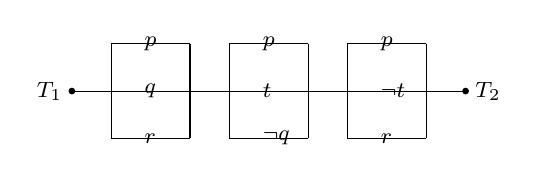
\begin{tikzpicture}[baseline=(start.base), every node/.style={font=\footnotesize}]
        % Coordinates for Main Line
        \coordinate (start) at (0,0);
        \node[left] at (start) {$T_1$};
        \draw[fill] (start) circle (1pt);
        
        % Block 1 (p, q, r)
        \draw (start) -- (0.5,0);
        \draw (0.5,0.6) -- (0.5,-0.6);
        \draw (0.5,0.6) -- (0.8,0.6) node[right] {$p$} -- (1.5,0.6);
        \draw (0.5,0)   -- (0.8,0)   node[right] {$q$} -- (1.5,0);
        \draw (0.5,-0.6) -- (0.8,-0.6) node[right] {$r$} -- (1.5,-0.6);
        \draw (1.5,0.6) -- (1.5,-0.6);
        \draw (1.5,0) -- (2.0,0);
        
        % Block 2 (p, t, ~q)
        \draw (2.0,0.6) -- (2.0,-0.6);
        \draw (2.0,0.6) -- (2.3,0.6) node[right] {$p$} -- (3.0,0.6);
        \draw (2.0,0)   -- (2.3,0)   node[right] {$t$} -- (3.0,0);
        \draw (2.0,-0.6) -- (2.3,-0.6) node[right] {$\neg q$} -- (3.0,-0.6);
        \draw (3.0,0.6) -- (3.0,-0.6);
        \draw (3.0,0) -- (3.5,0);
        
        % Block 3 (p, ~t, r)
        \draw (3.5,0.6) -- (3.5,-0.6);
        \draw (3.5,0.6) -- (3.8,0.6) node[right] {$p$} -- (4.5,0.6);
        \draw (3.5,0)   -- (3.8,0)   node[right] {$\neg t$} -- (4.5,0);
        \draw (3.5,-0.6) -- (3.8,-0.6) node[right] {$r$} -- (4.5,-0.6);
        \draw (4.5,0.6) -- (4.5,-0.6);
        
        % End Node
        \draw (4.5,0) -- (5.0,0);
        \node[right] at (5.0,0) {$T_2$};
        \draw[fill] (5.0,0) circle (1pt);
    \end{tikzpicture}
    \end{minipage}
    
    \vspace{0.8cm}
    
    % --- Circuit C2 ---
    \noindent
    \begin{minipage}{\textwidth}
    \raggedright
    \makebox[0.8cm][l]{$C2:$}
    \begin{tikzpicture}[baseline=(start.base), every node/.style={font=\footnotesize}]
        % Coordinates for Main Line
        \coordinate (start) at (0,0);
        \node[left] at (start) {$T_1$};
        \draw[fill] (start) circle (1pt);
        
        \draw (start) -- (0.5,0);
        \draw (0.5,0.6) -- (0.5,-0.6);
        
        % Upper branch (p)
        \draw (0.5,0.6) -- (0.8,0.6) node[right] {$p$} -- (4.5,0.6);
        
        % Lower branch (r connected to sub-parallel t and ~q)
        \draw (0.5,-0.6) -- (0.8,-0.6) node[right] {$r$} -- (1.5,-0.6);
        
        % Sub-parallel block
        \draw (1.5,-0.2) -- (1.5,-1.0);
        \draw (1.5,-0.2) -- (1.8,-0.2) node[right] {$t$} -- (2.5,-0.2);
        \draw (1.5,-1.0) -- (1.8,-1.0) node[right] {$\neg q$} -- (2.5,-1.0);
        \draw (2.5,-0.2) -- (2.5,-1.0);
        
        % Connecting lower branch back up
        \draw (2.5,-0.6) -- (4.5,-0.6);
        
        % Right closing boundary
        \draw (4.5,0.6) -- (4.5,-0.6);
        \draw (4.5,0) -- (5.0,0);
        \node[right] at (5.0,0) {$T_2$};
        \draw[fill] (5.0,0) circle (1pt);
    \end{tikzpicture}
    \end{minipage}

    \vspace{0.6cm}
    \noindent (Show details of logical reasoning \& rules).
\mk{15} \yr{CSE 103 | L-1/T-2 | 2013--14}  



%% 2023-24
\item Determine if the following statement is a tautology using a truth table:
\[
  p \land (p \land q) \iff (p \implies q)
\]
\mk{6} \yr{CSE 103 | L-1/T-2 | 2012--13}

%% 2012-13
\item Using a truth table, show whether the following argument is valid:
\[
  p \to q \lor r, \quad \lnot q \lor \lnot r \quad \therefore\; \lnot p \lor \lnot r
\]
\mk{10} \yr{CSE 103 | L-1/T-2 | 2012--13}

%% 2012-13
\item Determine whether the sentence $\lnot(p \lor \lnot(\lnot q \lor \lnot r))$ is logically equivalent to $(p \lor q) \implies \lnot(p \lor r)$.
\mk{10} \yr{CSE 103 | L-1/T-2 | 2012--13}

%% 2013-14
\item Argue whether the following sentences correspond to propositions:
\begin{enumerate}
  \item ``Shohag is a liar.''
  \item ``I am a liar.''
  \item ``There is a cook in a village who cooks food for those who do not cook for themselves.''
\end{enumerate}
For each sentence, determine whether it is a proposition, and if so, whether its truth value can be determined. Note that sentence (ii) and (iii) involve self-referential and paradoxical constructions — explain what makes them unusual.
\mk{3+3+3} \yr{CSE 103 | L-1/T-2 | 2011--12}

%% 2012-13
\item A virus is a malicious program that causes harm to your PC. An anti-virus is a program that tries to find a virus and kills it if found. One of your classmates has developed a virus called ``V1'' that no anti-virus can kill. On the other hand, you have developed an anti-virus program ``KillAll'' that can kill every virus it finds. Now your PC is infected with V1 and you have loaded KillAll. What will happen? Analyse this logically.
\mk{5} \yr{CSE 103 | L-1/T-2 | 2010--11}

%% 2020-21
\item Suppose you are dealing with 3 persons, A, B and C. One of them always tells the truth (Knight), one always lies (Knave), and one either lies or tells the truth (Spy). For the following scenarios, determine the identities of each person with appropriate arguments.
\begin{enumerate}
  \item A says: ``I am a knight.''; B says: ``That is true.''; C says: ``I am the spy!''
  \item A says: ``B is the spy!''; B says: ``No, C is the spy!''; C says: ``No, B is definitely the spy.''
\end{enumerate}
\mk{10} \yr{CSE 103 | L-1/T-2 | 2009--10}

%% 2010-11
\item In a class of 4 students (Romeo, Juliet, Tom and Jerry), the teacher did not call rolls; instead, he took signatures on an attendance sheet. One day, after leaving the classroom, he noticed that all 4 signatures are present but he knew that one of the students was absent — meaning someone gave a proxy signature for the absentee. In this case, two students are guilty: one who gave the proxy and another who is the absentee who requested the proxy. In the next class, he asked each student individually and got the following responses:
\begin{itemize}[leftmargin=1.8em,itemsep=2pt,label={$\bullet$}]
  \item Romeo: ``Juliet is not involved in this guilt.''
  \item Juliet: ``Romeo is not involved.''
  \item Tom: ``Jerry is involved in this guilt.''
  \item Jerry: ``Tom is not involved.''
\end{itemize}
Exactly one of them told a lie. From this information, find out the one who is involved in the guilt for sure.
\mk{15} \yr{CSE 103 | L-1/T-2 | 2008--09}

%% 2008-09
\item There are 100 statements, numbered 1 to 100, where the $i$-th statement says: ``Exactly $i$ statements are false.'' For example: (1) Exactly 1 statement is false; (2) Exactly 2 statements are false; \ldots; (100) Exactly 100 statements are false. Find out which statements are false and which are true. Justify your answer.
\mk{11} \yr{CSE 103 | L-1/T-2 | 2008--09}

%% 2009-10
\item Let $p$, $q$, $r$, $s$, $t$ denote the following statements:
\begin{itemize}[leftmargin=1.8em,itemsep=1pt,label={$\bullet$}]
  \item $p$: I finish my computer program
  \item $q$: I shall play football
  \item $r$: The sun is shining
  \item $s$: The humidity is low
  \item $t$: I shall go to newmarket
\end{itemize}
Write each of the following in symbolic form:
\begin{enumerate}
  \item If the sun is shining, then I shall play football.
  \item Finishing my computer program is necessary for my playing football.
  \item Low humidity and sunshine are sufficient for my playing football.
  \item Finishing my computer program is not necessary for my going to newmarket.
  \item I shall play football only if the sun is shining.
  \item The sun is shining if and only if the humidity is low.
  \item I do not care anything; in any circumstances I will go to newmarket and will play football.
  \item If the sun is not shining and the humidity is not low, then I will neither play football nor go to newmarket.
  \item My playing football implies that the humidity is low, which in turn implies that I have finished my computer program.
\end{enumerate}
\mk{10} \yr{CSE 103 | L-1/T-2 | 2006--07}

%% 2006-07
\item State the principle of Duality. Apply this principle to:
\[
  \bigl((p \lor q) \land (\lnot p \lor \lnot q)\bigr) \iff \bigl((p \land \lnot q) \lor (\lnot p \land q)\bigr).
\]
Show by truth table that the dual you have found is correct.
\mk{10} \yr{CSE 103 | L-1/T-2 | 2006--07}



%% 2020-21
\end{enumerate}

%%──────────────────────────────────────────────────────────────────────
\subtopic{cA}{Predicate Logic}
\label{sub:s1-predlogic}

\begin{enumerate}


\item Determine the truth value of each of the following statements, where the domain of each variable is the set of all real numbers. For each statement, state whether it is true or false and justify your answer.
\begin{enumerate}
    \item $\forall x (x \neq 0 \rightarrow \exists y (xy = 1))$
    \item $\exists x \forall y (y \neq 0 \rightarrow xy = 1)$
    \item $\forall x \exists y (x + y = 1)$
    \item $\forall x \exists y (x + y = 2 \wedge 2x - y = 1)$
    \item $\forall x \forall y \exists z \left(z = \frac{x + y}{2}\right)$
\end{enumerate}
\mk{10} \yr{CSE 103 | L-1/T-I | 2024--25}


%% 2008-09
\item Express the following statements using predicates and quantifiers:
\begin{enumerate}
  \item There is a smallest positive integer.
  \item There is no smallest positive real number.
  \item There are infinitely many prime numbers.
  \item Every even number is the sum of two prime numbers.
\end{enumerate}
\mk{10} \yr{CSE 103 | L-1/T-1 | 2023--24, 2009--10}

%% 2006-07
\item Translate each of the following propositions into an English sentence. The relevant predicates are defined over the set $P$ of all people: $A(x)$: ``$x$ is teaching CSE 105''; $T(x)$: ``$x$ is taking CS 473''; $F(x)$: ``$x$ has a Facebook page''; $C(x)$: ``$x$ likes to cook.''
\begin{enumerate}
  \item $\exists x \in P\,[A(x) \land C(x)]$
  \item $\lnot\forall x \in P\,[T(x) \to (F(x) \lor C(x))]$
\end{enumerate}
\mk{6+6} \yr{CSE 103 | L-1/T-2 | 2020--21}  

%% 2015-16
\item Suppose that the domain of the propositional function $P(x)$ consists of the integers $-2, -1, 0, 1, 2$. Write down each of the following propositions using only disjunctions, conjunctions, and negations (i.e., expand the quantifiers explicitly):
\begin{enumerate}
  \item $\exists x\, P(x)$
  \item $\forall x\, P(x)$
  \item $\exists x\, \lnot P(x)$
  \item $\forall x\, \lnot P(x)$
  \item $\lnot \exists x\, P(x)$
  \item $\lnot \forall x\, P(x)$
  \item $\lnot \forall x\, \lnot P(x)$
\end{enumerate}
\mk{7} \yr{CSE 103 | L-1/T-2 | 2017--18}  


%% 2011-12
\item Determine the truth value of each statement if the universe is nonzero integers:
\begin{enumerate}
  \item $\exists x\, \exists y\, [(3x + y = 8) \land (2x - y = 7)]$
  \item $\forall x\, \exists y\, [x \cdot y = 2]$
\end{enumerate}
\mk{8+8} \yr{CSE 103 | L-1/T-2 | 2016--17}

%% 2017-18
\item Translate the following nested quantification into an English statement that expresses a mathematical fact, assuming all real numbers are in the domain:
\[
  \forall x\, \forall y\, \bigl(((x \geq 0) \land (y < 0)) \to (x - y > 0)\bigr).
\]
\mk{7} \yr{CSE 103 | L-1/T-2 | 2015--16}

%% 2016-17
\item Find the statements in symbolic form using the open statements: $p(x)$: $x > 0$; $q(x)$: $x$ is even; $r(x)$: $x$ is a perfect square; $s(x)$: $x$ is exactly divisible by 4; $t(x)$: $x$ is exactly divisible by 5. These predicates apply over the universe of all integers.
\begin{enumerate}
  \item There exists a positive integer that is even.
  \item If $x$ is even and $x$ is a perfect square, then $x$ is divisible by 4.
\end{enumerate}
\mk{8} \yr{CSE 103 | L-1/T-2 | 2013--14}

%% 2013-14
\item Let $P(x)$, $Q(x)$, and $R(x)$ be the statements ``$x$ is a clear explanation'', ``$x$ is satisfactory'', and ``$x$ is an excuse'' respectively. The domain consists of all statements. Using quantifiers, logical connectives, and $P(x)$, $Q(x)$, $R(x)$, express and analyse: All clear explanations are satisfactory; Some excuses are unsatisfactory; Some excuses are not clear explanations. Does the third follow from the first two?
\mk{5} \yr{CSE 103 | L-1/T-2 | 2013--14}

%% 2013-14
\item Use quantifiers and predicates to express the fact that $\lim_{x \to a} f(x)$ does not exist, where $f(x)$ is a real-valued function of a real variable $x$, and $a$ belongs to the domain of $f$.
\mk{5} \yr{CSE 103 | L-1/T-2 | 2013--14, 2011--12}  

%% 2023-24
\item Express the following sentences using quantifiers. Use the variable $s$ for student, $c$ for course, $d$ for department. Use the predicate $\textit{register}(s,c)$ to mean ``student $s$ registered to course $c$'', $\textit{course}(c,d)$ to mean ``course $c$ is offered by department $d$'', $\textit{student}(s,d)$ to mean ``student $s$ is enrolled in department $d$''. The domain of $s$ is the set of all students of all departments, domain of $c$ is the set of all courses, and domain of $d$ is the set of all departments.
\begin{enumerate}
  \item There is a student who has taken all courses of the CSE department.
  \item There is a student who has registered for all courses of all departments.
  \item There is a student who has registered for at least one course from every department.
  \item All students registered for one particular course of the CSE department.
\end{enumerate}
\mk{12} \yr{CSE 103 | L-1/T-2 | 2012--13}

%% 2013-14
\item Translate each of the following statements into logical expressions using quantifiers, predicates, and logical connectives. Use $P(x)$ to mean ``$x$ is perfect'' and $F(x)$ to mean ``$x$ is your friend.''
\begin{enumerate}
  \item No one is perfect.
  \item Not everyone is perfect.
  \item All your friends are perfect.
  \item One of your friends is perfect.
  \item Everyone is your friend.
  \item Not everybody is your friend or someone is not perfect.
\end{enumerate}
\mk{6+6} \yr{CSE 103 | L-1/T-2 | 2011--12}

%% 2012-13
\item Suppose $\mathbb{Z}^+$ and $\rho$ denote the set of positive integers and prime numbers respectively. Translate the statement ``The set of prime numbers is unbounded'' into first-order logic. Also negate the statement.
\mk{10} \yr{CSE 103 | L-1/T-2 | 2010--11}

%% 2020-21
\item Write down the necessary condition and the sufficient condition which are equivalent to the following statement: $p \to q$.
\mk{5} \yr{CSE 103 | L-1/T-2 | 2008--09}

%% 2008-09
\item Translate the following statements into English, where $C(x)$ denotes ``$x$ is a comedian'', $F(x)$ denotes ``$x$ is funny'', and the universe of discourse consists of all people:
\begin{enumerate}
  \item $\forall x,\, (C(x) \to F(x))$
  \item $\forall x,\, (C(x) \land F(x))$
  \item $\exists x,\, (C(x) \to F(x))$
  \item $\exists x,\, (C(x) \land F(x))$
\end{enumerate}
\mk{2+2+2+2} \yr{CSE 103 | L-1/T-2 | 2008--09}

%% 2008-09
\item Justify the following arguments:
\begin{center}
  \begin{tabular}{ll}
(i) \quad 
$\begin{aligned}[t]
    & p \rightarrow r \\
    & r \rightarrow s \\
    & t \lor \neg s \\
    & \neg t \lor u \\
    & \neg u \\
    \hline
    \therefore \quad & p
\end{aligned}$ 
& \qquad \qquad (ii) \quad 
$\begin{aligned}[t]
    & \forall_x [p(x) \lor q(x)] \\
    & \exists x \neg p(x) \\
    & \forall x [\neg q(x) \lor r(x)] \\
    & \forall x [s(x) \rightarrow \neg r(x)] \\
    \hline
    \therefore \quad & \exists x \neg s(x)
\end{aligned}$
\end{tabular}
\end{center}
\mk{7+8} \yr{CSE 103 | L-1/T-2 | 2008--09}

%% 2010-11
\item Let the universe of $x$, $y$, $z$ be the set of integers. Find the truth or falsity for each of the following statements. For each false statement, give an argument or counter-example as necessary.
\begin{enumerate}
  \item $\forall x\; \exists!\, z\; \forall y\;[x + y = z]$
  \item $\forall x\; \forall y\; \exists!\, z\;[x + y = z]$
  \item $\forall y\; \exists!\, x\;[x \cdot y = 0]$
  \item $\forall x\; \forall y\;[x < y \implies \exists z\;[x < z < y]]$
\end{enumerate}
\mk{10} \yr{CSE 103 | L-1/T-2 | 2006--07}



\end{enumerate}

%%──────────────────────────────────────────────────────────────────────
\subtopic{cA}{Arguments \& Rules of Inference}
\label{sub:s1-proplogic-inference}

\begin{enumerate}

\item For each of the following arguments, determine whether the argument is correct or incorrect and explain why.
\begin{enumerate}
  \item All students in this class understand logic. Mr.\ X is a student in this class. Therefore, Mr.\ X understands logic.
  \item Every computer science major takes discrete mathematics. Mr.\ X is taking discrete mathematics. Therefore, Mr.\ X is a computer science major.
\end{enumerate}
\mk{5} \yr{CSE 103 | L-1/T-1 | 2023--24}

\item Prove the validity of the argument/formula below. Note that this can be established either by using proof by contradiction or via rules of inference:
\[
  (\lnot p \lor q) \to r,\quad r \to (s \lor t),\quad \lnot s \land \lnot u,\quad \lnot u \to \lnot t \quad \therefore\; p
\]
\mk{15} \yr{CSE 103 | L-1/T-2 | 2016--17, 2013--14, 2006--07}

\item Find if the following argument is valid: ``If the band could not play rock music or the snacks were not delivered on time, then the party would have been cancelled and Maria would be angry. If the party were cancelled, then refunds would have had to be made. No refunds were made. Therefore, the band could play rock music.'' Express the argument formally and verify its validity.
\mk{12} \yr{CSE 103 | L-1/T-2 | 2013--14}  

\item Using rules of inference, prove the validity of the following argument. Write the reason on the right-hand side for each step.
\[
  \bigl[p \land (p \to q) \land (s \lor r) \land (r \to \lnot q)\bigr] \to (s \lor t)
\]
\mk{7.5} \yr{CSE 103 | L-1/T-2 | 2006--07}

\item Decide whether the following arguments are valid or invalid. Clearly justify your answer.
\begin{enumerate}
  \item If Sadia is older than Soheli, then Sadia is at least 34 years old. Sadia is 34 years old. Therefore, Sadia is older than Soheli.
  \item If it rains, then I will not go to job. It is not raining. Therefore, I will go to job.
\end{enumerate}
\mk{10} \yr{CSE 103 | L-1/T-2 | 2006--07}

\end{enumerate}

%%──────────────────────────────────────────────────────────────────────
\subtopic{cA}{Mathematical Reasoning}
\label{sub:s1-reasoning}

\begin{enumerate}

\item Write the numbers $1, 2, \ldots, 2n$ on a blackboard, where $n$ is an odd integer. Pick any two numbers $j$ and $k$, write $|j - k|$ on the board and erase $j$ and $k$. Continue this process until only one integer is left on the board. Prove that this integer must be odd.
\mk{7} \yr{CSE 103 | L-1/T-2 | 2015--16}

\end{enumerate}

%% ── S2: Proof Techniques ──────────────────────────────────────────────
\section{S2 --- Proof Techniques}
\label{sec:S2}
\markboth{S2 --- Proof Techniques}{}

%%──────────────────────────────────────────────────────────────────────
\subtopic{cA}{Direct Proof \& Counterexamples}
\label{sub:s2-direct}

\begin{enumerate}

\item Prove that for an integer $n$, $n$ is even if and only if $n^2$ is even.
\mk{5} \yr{CSE 103 | L-1/T-1 | 2023--24, 2010--11}

\item Is $0.12121212\ldots$ a rational number? Justify your answer.
\mk{5} \yr{CSE 103 | L-1/T-2 | Jan 2020}

\item Prove or disprove that for every integer $n$, $4n + 7$ is odd.
\mk{7} \yr{CSE 103 | L-1/T-2 | 2016--17, 2012--13}

\item Prove that there is no positive integer $n$ such that $n^2 + n^3 = 100$.
\mk{7} \yr{CSE 103 | L-1/T-2 | 2013--14}

\item Prove the following statement: $\forall$ odd $n$, $\exists\, m$ such that $n^2 = 8m + 1$.
\mk{15} \yr{CSE 103 | L-1/T-2 | 2010--11, 2013--14} 

\end{enumerate}


%%──────────────────────────────────────────────────────────────────────
\subtopic{cA}{Proof by Contrapositive \& Indirect Proofs}
\label{sub:s2-contrapositive}

\begin{enumerate}

\item Let $n \in \mathbb{Z}$. Prove that if $n^2 - 6n + 5$ is even, then $n$ is odd.
\mk{6} \yr{CSE 103 | L-1/T-1 | 2022--23}

\item Prove that if $n$ is an integer and $5n + 2$ is odd, then $n$ is odd.
\mk{5} \yr{CSE 103 | L-1/T-2 | 2013--14} \yr{CSE 103 | L-1/T-2 | 2017--18}

\item Prove that for any two integers $a$ and $b$, if $ab$ is even, then $a$ is even or $b$ is even.
\mk{9} \yr{CSE 103 | L-1/T-2 | 2012--13} \yr{CSE 103 | L-1/T-2 | 2023--24}

\item Consider the following statement: If $f(x) = x^2 - 7$ and $a \neq b$, then $f(a) \neq f(b)$. Form the contrapositive of the statement. Prove or disprove the original statement.
\mk{10} \yr{CSE 103 | L-1/T-2 | 2010--11}

\item What do you mean by an \textbf{indirect proof}? Give an indirect proof of the theorem: ``If $3n + 2$ is odd, then $n$ is odd.''
\mk{2+4} \yr{CSE 103 | L-1/T-2 | 2008--09}

\item Prove the following statement (note that it can be approached via contrapositive or contradiction): If $m$ is an even integer, then $m + 7$ is odd.
\mk{7.5} \yr{CSE 103 | L-1/T-2 | 2006--07}

\end{enumerate}


%%──────────────────────────────────────────────────────────────────────
\subtopic{cA}{Proof by Contradiction \& Existence Proofs}
\label{sub:s2-contradiction}

\begin{enumerate}

\item Prove that both $\sqrt{2}$ and $\sqrt{3}$ are irrational. 
\mk{10} \yr{CSE 103 | L-1/T-1 | 2022--23} \yr{CSE 103 | L-1/T-2 | 2020--21, Jan 2020}

\item Suppose $p \in \mathbb{N}$ and $p \geq 2$. Prove by contradiction that if $2^p - 1$ is prime, then $p$ is prime.
\mk{6} \yr{CSE 103 | L-1/T-1 | 2022--23} \yr{CSE 103 | L-1/T-1 | 2008--09}

\item Discuss constructive and non-constructive proof techniques. Show full arguments (constructive, non-constructive, or word-problem format) to prove or justify whether an irrational number raised to an irrational power can be rational.
\mk{15} \yr{CSE 103 | L-1/T-2 | 2009--10} \variant{2024--25, 2022--23, 2021--22, Jan 2020, 2017--18, 2013--14, 2010--11}

\item Prove by contradiction that $\sqrt[3]{2}$ is irrational.
\mk{7} \yr{CSE 103 | L-1/T-2 | 2013--14}  

\item Prove by contradiction that $\sqrt{7}$ is irrational.
\mk{8} \yr{CSE 103 | L-1/T-2 | 2009--10} \yr{CSE 103 | L-1/T-2 | 2022--23}

\item Prove that ``There is no largest prime number.'' Mention the name of the proof technique you used.
\mk{10} \yr{CSE 103 | L-1/T-2 | 2008--09}

\end{enumerate}


%%──────────────────────────────────────────────────────────────────────
\subtopic{cA}{Mathematical Induction}
\label{sub:s2-induction}

\begin{enumerate}


%% Session: 2024-2025
\item Joey has bought an item costing $X$ dollars from a shop and now needs to pay exactly $X$ dollars. He has one bundle of 4-dollar notes and another bundle of 7-dollar notes, and in total he has more than $X$ dollars on him. However, the shopkeeper will only accept the exact amount $X$. Joey is not sure whether he can make exactly $X$ dollars using his two bundles of notes, so he calls his genius friend Ross for help. Ross proves that as long as $X \ge 18$, Joey can always make exactly $X$ dollars from her bundles. Prove by strong induction that for all integers $X \ge 18$, Joey can form exactly $X$ dollars using some combination of 4-dollar and 7-dollar notes.
\mk{10} \yr{CSE 103 | L-1/T-I | 2024--25}

%% 2010-11
\item Prove by induction that given an unlimited supply of 5-taka and 3-taka stamps, we can form any postage of amount $\geq 8$ taka.
\mk{10} \yr{CSE 103 | L-1/T-1 | 2023--24}

%% 2022-23
\item Consider the following inductive proof that claims to show ``All persons in Bangladesh are bald,'' assuming at least one person in Bangladesh is bald.\\[6pt]

\begin{tcolorbox}[colback=gray!5,colframe=gray!40,boxrule=0.5pt,arc=4pt,
  left=8pt,right=8pt,top=6pt,bottom=6pt]
  \small
\textit{Proof.} We will first prove $P(n)$ where $P(n)$ = ``For all groups of $n$ persons, whenever one person is bald, then all persons are bald.'' We proceed as follows.\\[3pt]
\textbf{Base case:} $P(1)$ is clearly true.\\[3pt]
\textbf{Induction step:} Suppose $P(k)$ is true for all $1 \leq k \leq n$; we wish to show $P(n+1)$ is true as well. Given a set $W$ of $n+1$ persons in which $x \in W$ is bald, take any two proper subsets $A, B \subset W$ (in particular $|A|, |B| < n+1$) such that they both contain the bald person ($x \in A$; $x \in B$), and $A \cup B = W$ (no one is left out). Applying the induction hypothesis to $A$ and $B$, we conclude that all the persons in $A$ and $B$ are bald, and so everyone in $W$ is bald.\\[3pt]
Finally, if we now consider $W$ to be the set of all persons in Bangladesh, the result follows. $\square$
\end{tcolorbox}
Determine what is wrong with the above inductive proof.
\mk{12} \yr{CSE 103 | L-1/T-1 | 2022--23}


%% 2022-23
\item There are two piles of books. Two players take turns removing any positive number of books they want from \textbf{one} of the two piles. The player who removes the last book wins the game. Prove by induction that if the two piles have the same number of books initially, the second player will always win.
\mk{10} \yr{CSE 103 | L-1/T-1 | 2022--23}

%% 2022-23
\item Prove by weak induction that postage of $n \geq 18$ taka can be formed using just 4-taka and 7-taka stamps.
\mk{10} \yr{CSE 103 | L-1/T-1 | 2022--23}

%% Session: 2021-2022
\item A polygon is said to be convex if any line joining two vertices lies within the polygon or on its boundary and a diagonal is a line joining any two non-adjacent vertices in the polygon. Now deduce a proof (by mathematical induction) for the statement: In a convex polygon with $n \ge 4$ vertices, the maximum number of diagonal that can be drawn is $\frac{1}{2} \times n \times (n - 3)$.
\mk{10} \yr{CSE 103 | L-1/T-I | 2021--22, Jan 2021}

%% Session: 2021-2022
\item Determine what amount can you form with 5 and 2 Taka notes and then prove that by (i) strong and (ii) weak induction.
\mk{15} \yr{CSE 103 | L-1/T-I | 2021--22}

%% Session: 2021-2022
\item Using well ordering principle, show that $\sqrt{2}$ is irrational.
\mk{10} \yr{CSE 103 | L-1/T-I | 2021--22}


%% Jan 2021
\item Prove that the greatest amount of postage you cannot make exactly using 4-taka and 9-taka stamps is 23 taka.
\mk{10} \yr{CSE 103 | L-1/T-2 | Jan 2021}

%% Jan 2021
\item Joey learned the concept of Mathematical Induction from Chandler. Now, Joey has come up with a proof of the `fact' that for all non-negative integers $n$, ``$n^2 + n$ is odd''. He wrote the following arguments:

\begin{tcolorbox}[colback=gray!5,colframe=gray!40,boxrule=0.5pt,arc=4pt,
  left=8pt,right=8pt,top=6pt,bottom=6pt]
\small Let $P(n)$ be the statement ``$n^2 + n$ is odd''. We will prove that $P(n)$ is true for all $n \in \mathbb{N}$. Suppose for induction that $P(k)$ is true, that is, $k^2 + k$ is odd. Now consider the statement $P(k+1)$. Now $(k+1)^2 + (k+1) = k^2 + 2k + 1 + k + 1 = k^2 + k + 2k + 2$. By the inductive hypothesis, $k^2 + k$ is odd, and of course $2k + 2$ is even. An odd plus an even is always odd, therefore $(k+1)^2 + (k+1)$ is odd. Therefore, by the principle of mathematical induction, $P(n)$ is true for all $n \in \mathbb{N}$.
\end{tcolorbox}

\vspace{4pt}
Chandler is baffled by the proof. Help Chandler find the flaw(s) in the above argument and explain the issue elaborately.
\mk{10} \yr{CSE 103 | L-1/T-2 | Jan 2021, 2020}

%% Jan 2020
\item You have bought something worth $X$ taka from a shop and need to pay the exact amount. You have one bundle of 2-taka notes and another bundle of 5-taka notes, and you have more than $X$ taka with you. But the shopkeeper only accepts the exact amount — he will only accept exactly $X$ taka. You called your genius little brother for help, and he proved to you that if $X \geq 4$, then you don't need to worry at all. Provide the proof:
\begin{enumerate}
  \item Using strong induction.
  \item Using weak induction.
\end{enumerate}
\mk{20} \yr{CSE 103 | L-1/T-2 | Jan 2020}


%% 2006-07
\item Explain the different steps needed to prove universal statements using the Well-Ordering Principle.
\mk{10} \yr{CSE 103 | L-1/T-2 | 2020--21}

%% 2020-21
\item Using the principle of mathematical induction, prove that $2^{2n} - 1$ is divisible by 3 for all $n \geq 1$.
\mk{15} \yr{CSE 103 | L-1/T-2 | 2020--21}  

%% 2016-17
\item Recently, Chandler enrolled in a discrete mathematics course and after a few lessons got intrigued with the concept of mathematical induction. Chandler decided to teach Joey the concept. Joey was also intrigued. The next day, Joey came up with a ``proof'' of the fact that for all values of $n$, $n + 3 = n + 7$. He wrote the following arguments using mathematical induction:
\begin{tcolorbox}[breakable,colback=gray!5,colframe=gray!40,boxrule=0.5pt,arc=4pt,
  left=8pt,right=8pt,top=6pt,bottom=6pt]
  \small
Let $P_n$ be the statement that $n + 3 = n + 7$. We will prove that $P_n$ is true for all $n \in \mathbb{N}$. Assume, for induction, that $P_k$ is true. That is, $k + 3 = k + 7$. We must show that $P_{k+1}$ is true. Now since $k + 3 = k + 7$, adding 1 to both sides we get $k + 3 + 1 = k + 7 + 1$. After regrouping we easily get $(k+1) + 3 = (k+1) + 7$. But this is simply $P_{k+1}$. Thus by the principle of mathematical induction, $P_n$ is true for all $n \in \mathbb{N}$.
\end{tcolorbox}
Find out the flaw(s) in the above argument.
\mk{10} \yr{CSE 103 | L-1/T-2 | 2017--18}

%% 2017-18
\item Suppose you have solved a puzzle where the goal is to tile a big square with trominos (L-shaped tiles covering three squares). An $8 \times 8$ puzzle has 4 trominos placed at arbitrary locations. Prove that for any $2^n \times 2^n$ puzzle, a tiling with trominos is possible with only one square unfilled in the middle. Then argue that $2^{2n} - 1$ is divisible by 3.
\begin{center}
  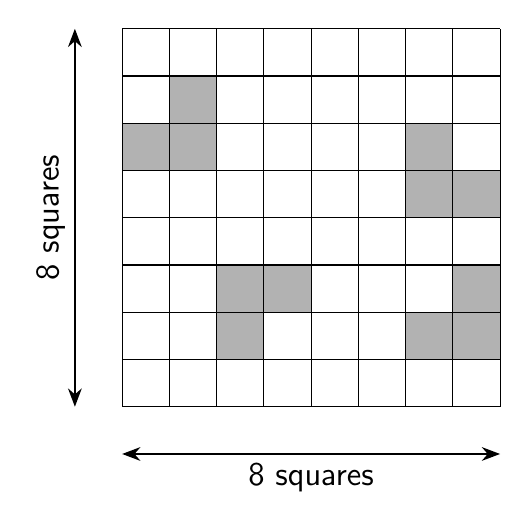
\begin{tikzpicture}[scale=0.6, >=Stealth]

    % ==========================================
    % SHADED SQUARES (Coordinates from bottom-left (0,0) to top-right (8,8))
    % ==========================================
    \begin{scope}[fill=gray!60]
        % Top-left cluster
        \fill (1,6) rectangle (2,7);
        \fill (0,5) rectangle (1,6);
        \fill (1,5) rectangle (2,6);
        
        % Middle-right cluster
        \fill (6,5) rectangle (7,6);
        \fill (6,4) rectangle (7,5);
        \fill (7,4) rectangle (8,5);
        
        % Bottom-left/middle cluster
        \fill (2,2) rectangle (3,3);
        \fill (3,2) rectangle (4,3);
        \fill (2,1) rectangle (3,2);
        
        % Bottom-right cluster
        \fill (7,2) rectangle (8,3);
        \fill (6,1) rectangle (7,2);
        \fill (7,1) rectangle (8,2);
    \end{scope}

    % ==========================================
    % GRID LINES (8x8)
    % ==========================================
    \draw[step=1cm, black, thin] (0,0) grid (8,8);

    % ==========================================
    % DIMENSION ARROWS & LABELS
    % ==========================================
    % Left vertical indicator
    \draw[<->, thick] (-1,0) -- (-1,8);
    \node[rotate=90, above, font=\large\sffamily] at (-1,4) {8 squares};
    
    % Bottom horizontal indicator
    \draw[<->, thick] (0,-1) -- (8,-1);
    \node[below, font=\large\sffamily] at (4,-1) {8 squares};

\end{tikzpicture}
\end{center}

\mk{15} \yr{CSE 103 | L-1/T-2 | 2017--18}

%% 2017-18
\item With the help of the Well-Ordering Principle, prove that $\sqrt{2}$ is irrational.
\mk{10} \yr{CSE 103 | L-1/T-2 | 2017--18}  

%% 2012-13
\item Prove that the Fibonacci numbers follow the pattern odd, odd, even: that is, show that for any positive integer $m$, $F_{3m-2}$ and $F_{3m-1}$ are odd and $F_{3m}$ is even.
\mk{15} \yr{CSE 103 | L-1/T-2 | 2016--17}

%% 2016-17
\item Use induction to show that the Euclidean algorithm correctly computes the greatest common divisor (GCD) of two positive integers.
\mk{15} \yr{CSE 103 | L-1/T-2 | 2016--17}

%% 2017-18
\item Write down the principle of Mathematical Induction. Using induction, prove that for every $n \in \mathbb{Z}^+$ where $n \geq 14$, $n$ can be written as a sum of 3's and 8's.
\mk{10} \yr{CSE 103 | L-1/T-2 | 2013--14, 2010--11}

%% 2013-14
\item Prove that every positive integer can be uniquely factorized (Fundamental Theorem of Arithmetic).
\mk{15} \yr{CSE 103 | L-1/T-2 | 2013--14}

%% 2011-12
\item Prove or disprove the following statement: Any amount of postage greater than or equal to 20 cents can be formed using only 5-cent and 6-cent stamps.
\mk{12} \yr{CSE 103 | L-1/T-2 | 2012--13}

%% 2012-13
\item Using induction, prove that $3^n \geq n^3$ for all integers $n \geq 3$.
\mk{13} \yr{CSE 103 | L-1/T-2 | 2012--13}

%% 2013-14
\item If $n$ is a positive integer, then $n$ cents in change using quarters (25 cents), dimes (10 cents), nickels (5 cents), and pennies (1 cent): the optimal change representation has at most two dimes, at most one nickel, at most 4 pennies, and cannot have two dimes and a nickel simultaneously. Also, the amount of change in dimes, nickels, and pennies cannot exceed 24 cents. Prove these statements using a greedy/optimality argument.
\mk{15} \yr{CSE 103 | L-1/T-2 | 2011--12}  

%% 2023-24
\item Define a two-colouring for a set of regions as a way of assigning one of two colours to each region such that no two regions sharing a side have the same colour (for example, a chessboard is two-coloured). Prove by weak induction that the set of regions formed by $n$ infinite lines in the plane can always be two-coloured.
\mk{17} \yr{CSE 103 | L-1/T-2 | 2010--11}


%% 2009-10
\item Consider the following claim and an associated proof by induction. Identify the problem in the proof.
\begin{tcolorbox}[breakable,colback=gray!5,colframe=gray!40,boxrule=0.5pt,arc=4pt,
  left=8pt,right=8pt,top=6pt,bottom=6pt]
  \small
\textbf{Claim:} \framebox{\textbf{All positive integers are equal.}}

\medskip
\noindent
\textbf{Proof:} To prove the claim, we will prove by induction that, for all $n \in \mathbb{N}$, the following statement holds:

\vspace{0.3cm}
\noindent
($P(n)$) \hfill For any $x, y \in \mathbb{N}$, if $\max(x,y) = n$, then $x = y$. \hfill \mbox{}

\vspace{0.3cm}
\noindent
(Here $\max(x,y)$ denotes the larger of the two numbers $x$ and $y$, or the common value if both are equal.)

\medskip
\noindent
\textbf{Base step:} When $n = 1$, the condition in $P(1)$ becomes $\max(x,y) = 1$. But this forces $x = 1$ and $y = 1$, and hence $x = y$.

\medskip
\noindent
\textbf{Induction step:} Let $k \in \mathbb{N}$ be given and suppose $P(k)$ is true. We seek to show that $P(k+1)$ is true as well.

\vspace{0.3cm}
\noindent
Let $x, y \in \mathbb{N}$ such that $\max(x,y) = k+1$. Then $\max(x-1, y-1) = \max(x,y) - 1 = (k+1) - 1 = k$. By the induction hypothesis, it follows that $x-1 = y-1$, and therefore $x = y$. This proves $P(k+1)$, so the induction step is complete.

\medskip
\noindent
\textbf{Conclusion:} By the principle of induction, $P(n)$ is true for all $n \in \mathbb{N}$. In particular, since $\max(1,n) = n$ for any positive integer $n$, it follows that $1 = n$ for any positive integer $n$. Thus, all positive integers must be equal to 1.
\end{tcolorbox}
\mk{18} \yr{CSE 103 | L-1/T-2 | 2010--11}


%% 2008-09
\item Discuss proof by the Invariant Method with the help of an example.
\mk{7} \yr{CSE 103 | L-1/T-2 | 2009--10}

%% 2009-10
\item Identify the problem in the proof by induction.

\begin{tcolorbox}[breakable,colback=gray!5,colframe=gray!40,boxrule=0.5pt,arc=4pt,
  left=8pt,right=8pt,top=6pt,bottom=6pt]
  \small
\begin{center}
    \framebox[0.65\textwidth]{
        \parbox{0.6\textwidth}{
            \textbf{Claim:} For all $n \in \mathbb{N}$, \hfill $(\ast) \ \displaystyle\sum_{i=1}^{n} i = \frac{1}{2}\left(n + \frac{1}{2}\right)^2$
        }
    }
\end{center}


\noindent
\textbf{Proof:} We prove the claim by induction. \\[0.2cm]
\textbf{Base step:} When $n = 1$, $(\ast)$ holds. \\[0.2cm]
\textbf{Induction step:} Let $k \in \mathbb{N}$ and suppose $(\ast)$ holds for $n = k$. Then
\begin{align*}
    \sum_{i=1}^{k+1} i &= \sum_{i=1}^{k} i + (k + 1) \\
    &= \frac{1}{2}\left(k + \frac{1}{2}\right)^2 + (k + 1) \quad \text{(by ind. Hypothesis)} \\
    &= \frac{1}{2}\left(k^2 + k + \frac{1}{4} + 2k + 2\right) \quad \text{(by algebra)} \\
    &= \frac{1}{2}\left[\left(k + 1 + \frac{1}{2}\right)^2 - 3k - \frac{9}{4} + k + \frac{1}{4} + 2k + 2\right] \quad \text{(more algebra)} \\
    &= \frac{1}{2}\left(k + 1 + \frac{1}{2}\right)^2 \quad \text{(simplifying)}
\end{align*}

\noindent
Thus, $(\ast)$ holds for $n = k + 1$, so the induction step is complete. \\[0.2cm]
\textbf{Conclusion:} By the principle of induction, $(\ast)$ holds for all $n \in \mathbb{N}$.
\end{tcolorbox}
\mk{6} \yr{CSE 103 | L-1/T-2 | 2009--10}

%% 2010-11
\item Prove the following by mathematical induction:
\begin{enumerate}
  \item For any $2^n \times 2^n$ puzzle, there is a tiling using trominos with exactly one un-tiled square at the middle.
  \item Every amount of money greater than or equal to 7 Taka can be made from 2-Taka and 5-Taka notes.
\end{enumerate}
\mk{10+10} \yr{CSE 103 | L-1/T-2 | 2009--10}



%% Jan 2020
\item Using mathematical induction, prove the following:
\begin{enumerate}
  \item $\displaystyle\sum_{i=1}^{n} i \cdot i! = (n+1)! - 1$
  \item Let $n \in \mathbb{Z}^+$ where $n \neq 1, 3$. Prove that $n$ can be expressed as a sum of 2's and/or 5's.
\end{enumerate}
\mk{10+10} \yr{CSE 103 | L-1/T-2 | 2008--09}

%% 2009-10
\item State the Well-Ordering Principle. State and prove the Principle of Mathematical Induction. Why are the above two principles meaningless if they are defined using real numbers instead of integers?
\mk{10} \yr{CSE 103 | L-1/T-2 | 2006--07}

%% 2006-07
\item Prove by induction: For any positive integer $n \geq 24$, $n$ can be written as a sum of 5's and/or 7's.
\mk{10} \yr{CSE 103 | L-1/T-2 | 2006--07}

%% 2006-07
\item Prove by induction:
\begin{enumerate}
  \item For any positive integer $n$,
  \[
    \sum_{i=1}^{n} \frac{F_{i-1}}{2^i} = 1 - \frac{F_{n+2}}{2^n},
  \]
  where $F_i$ is the $i$-th Fibonacci number.
  \item If $a_0 = 1$, $a_1 = 1$, $a_2 = 1$, and $a_n = a_{n-1} + a_{n-3}$ for $n \geq 3$, then $a_{n+2} \geq (\sqrt{2})^n$ for all $n \geq 0$.
\end{enumerate}
\mk{5+5} \yr{CSE 103 | L-1/T-2 | 2006--07}

%% 2006-07
\item For $n \in \mathbb{Z}^+$, consider the statement
\[
  S(n):\; \sum_{i=1}^{n} i = \tfrac{1}{2}\!\left(n + \tfrac{1}{2}\right)^{\!2}.
\]
Prove that the truth of $S(k)$ implies the truth of $S(k+1)$ for all $k \in \mathbb{Z}^+$. Can we say from here that $S(n)$ is also true for all $n \in \mathbb{Z}^+$? Justify your answer. Is $S(n)$ true for some starting point $n_0 \in \mathbb{Z}^+$ and all $n \geq n_0$? Justify your answer. What can you say about the importance of the ``base case'' in a proof by mathematical induction?
\mk{15} \yr{CSE 103 | L-1/T-2 | 2006--07}


%% 2020-21
\end{enumerate}

%% ══════════════════════════════════════════════════════════════════════
%%  PART II — SET THEORY & RELATIONS
%% ══════════════════════════════════════════════════════════════════════
\secdivider{Part II}{Set Theory \& Relations}{cB}{cB}

%% ── S3: Set Theory ────────────────────────────────────────────────────
\section{S3 --- Set Theory}
\label{sec:S3}
\markboth{S3 --- Set Theory}{}

%%──────────────────────────────────────────────────────────────────────
\subtopic{cB}{Sets}
\label{sub:s3-sets}

\begin{enumerate}


%% 2009-10
\item Judge whether:
\begin{enumerate}
  \item An empty set is a subset of any set.
  \item Any set $S$ is a subset of itself.
\end{enumerate}
Justify each answer.
\mk{15} \yr{CSE 103 | L-1/T-2 | 2020--21}

%% 2020-21
\item Using an appropriate example with a Venn diagram, demonstrate that $A \cup (B \cap C) = (A \cup B) \cap (A \cup C)$.
\mk{10} \yr{CSE 103 | L-1/T-2 | 2020--21}

%% 2015-16
\item Use set-builder notation and logical equivalences to establish that $\overline{A \cap B} = \bar{A} \cup \bar{B}$.
\mk{7} \yr{CSE 103 | L-1/T-2 | 2015--16} 

%% 2013-14
\item Define function, inverse function, one-to-one function, and onto function with examples.
\mk{7} \yr{CSE 103 | L-1/T-2 | 2013--14} 


%% 2006-07
\item Prove De Morgan's law for sets: $\overline{A \cup B} = \bar{A} \cap \bar{B}$.
\mk{10} \yr{CSE 103 | L-1/T-2 | 2011--12}

%% 2011-12
\item Prove that the set of real numbers is an uncountable set.
\mk{13} \yr{CSE 103 | L-1/T-2 | 2011--12}


%% 2020-21
\item Define with examples: subset, proper subset, empty set, and power set.
\mk{10} \yr{CSE 103 | L-1/T-2 | 2006--07}

%% 2006-07
\item List all partitions of $A = \{a, b, c\}$.
\mk{5} \yr{CSE 103 | L-1/T-2 | 2006--07}

%% 2006-07
\item Let $S$ and $T$ be two subsets of a universe. Prove using laws of set theory (i.e., without using Venn diagrams or membership tables) that:
\[
  S \text{ and } T \text{ are disjoint if and only if } S \cup T = S \,\Delta\, T.
\]
\mk{15} \yr{CSE 103 | L-1/T-2 | 2006--07}

\end{enumerate}

%%──────────────────────────────────────────────────────────────────────
\subtopic{cB}{Functions}
\label{sub:s3-functions}

\begin{enumerate} 

%% Session: 2024-2025
\item If $A = \{a,b,c,d,e\}$ five distinct objects are to be distributed to $B = \{1,2,3,4\}$ four containers, then how many ways to distribute these distinct objects to the distinguishable four container? What will be the number of ways to distribute these distinct objects among four identical containers when no containers are empty? (Show the computation).
\mk{10} \yr{CSE 103 | L-1/T-I | 2024--25}

%% Session: 2024-2025
\item If a function $f: A \rightarrow B$ is invertible, and a function $g: B \rightarrow A$ satisfies $(g \circ f) = 1_A$ and $(f \circ g) = 1_B$ then, prove function $g$ is unique.
\mk{8} \yr{CSE 103 | L-1/T-I | 2024--25}

%% Session: 2024-2025
\item Let function $f: \mathbb{Z} \rightarrow \mathbb{R}$ be defined by $f(x) = x^2 + 5$ and function $g: \mathbb{R} \rightarrow \mathbb{R}$ defined by $g(x) = x^2 + 5$. Find $f^{-1}(S)$ and $g^{-1}(S)$ for various subsets of co-domain $\mathbb{R}$, where $S = [-4,5), [5,\infty)$.
\mk{6} \yr{CSE 103 | L-1/T-I | 2024--25}


%% 2011-12
\item If $f: A \to B$, $g: B \to C$ and $h: C \to D$, then justify that $(h \circ g) \circ f = h \circ (g \circ f)$, where the symbols carry the standard meaning.
\mk{10} \yr{CSE 103 | L-1/T-1 | 2023--24}

%% 2022-23
\item Justify the following statements regarding functions:
\begin{enumerate}
  \item A function $f$ can have an inverse only if $f$ is injective and surjective.
  \item $f$ and $g$ are two functions defined by $f: X \to Y$ and $g: Y' \to Z$. Then $g(f(x))$ is defined only if $Y \subseteq Y'$.
\end{enumerate}
\mk{4+4} \yr{CSE 103 | L-1/T-1 | 2022--23}

%% Jan 2021
\item If functions $f: \mathbb{R} \to \mathbb{R}$ and $g: \mathbb{R} \to \mathbb{R}$ are onto, is $c \cdot (f + g)$ also an onto function? (Here $c$ is a nonzero positive constant.) Explain your answer.
\mk{10} \yr{CSE 103 | L-1/T-2 | Jan 2021}


\item Let $S = \{1,2,3,4,5,6\}$, $f: S \to \mathbb{R}$ and $f = \{(1,7),(2,9),(3,11),(4,13),(5,15),(6,17)\}$. Let $g: \mathbb{Q} \to \mathbb{R}$ where $g(q) = 2q + 5$ for all $q \in \mathbb{Q}$, and $h: \mathbb{R} \to \mathbb{R}$ where $h(r) = 2r + 5$ for all $r \in \mathbb{R}$. Show that $f$ is a restriction of the function $h$ (from $\mathbb{R}$ to $S$).
\mk{6} \yr{CSE 103 | L-1/T-2 | Jan 2020}

%% 2006-07
\item Differentiate injective, bijective, and surjective functions using appropriate examples.
\mk{10} \yr{CSE 103 | L-1/T-2 | 2020--21}

%% 2020-21
\item Compare two composite functions denoted by $f \circ g$ and $g \circ f$ using appropriate examples.
\mk{13} \yr{CSE 103 | L-1/T-2 | 2020--21}

%% 2020-21
\item Judge whether the following statements are true or false. Justify each answer.
\begin{enumerate}
  \item If two elements in the domain of a function are equal, then their images in the co-domain are equal.
  \item If two elements in the co-domain of a function are equal, then their pre-images in the domain are also equal.
  \item A function can have the same output for more than one input.
\end{enumerate}
\mk{12} \yr{CSE 103 | L-1/T-2 | 2020--21}

%% Jan 2020
\item Define function, one-to-one function, onto function, and bijection. Show their differences using diagrams.
\mk{15} \yr{CSE 103 | L-1/T-2 | 2017--18}

%% 2017-18
\item Let $F$ be a function from a finite set $X$ to a finite set $Y$. If $n > 1$ and $|X| > n|Y|$, then prove that there exists an element of $Y$ that is the image under $F$ of at least $n+1$ elements of $X$.
\mk{10} \yr{CSE 103 | L-1/T-2 | 2017--18}  

%% 2023-24
\item For $A = \{1,2,3,4,5\}$, let $f: A \to \mathbb{R}$ be defined by $f = \{(1,10),(2,13),(3,16),(4,19),(5,22)\}$. Let $g: \mathbb{Q} \to \mathbb{R}$ where $g(q) = 3q + 7$ for all $q \in \mathbb{Q}$. Let $h: \mathbb{R} \to \mathbb{R}$ with $h(r) = 3r + 7$ for all $r \in \mathbb{R}$.
\begin{enumerate}
  \item Find the restriction of $g$ (from $\mathbb{Q}$) to $A$.
  \item Find the extension of $g$ (from $\mathbb{Q}$) to $\mathbb{R}$. Show the computation.
\end{enumerate}
\mk{8+8} \yr{CSE 103 | L-1/T-2 | 2016--17}

%% 2016-17
\item Let $A = \{1,2,3,4,5\}$, $B = \{w,x,y,z\}$, $A_1 = \{2,3,5\}$ (a subset of $A$), and $g: A_1 \to B$. In how many ways can $g$ be extended to a function $f: A \to B$?
\mk{8} \yr{CSE 103 | L-1/T-2 | 2016--17}

%% 2016-17
\item Consider a function $f: \mathbb{Z} \to \mathbb{Z}$ where $f(x) = 3x + 1$ for each $x \in \mathbb{Z}$. The range of $f$ is $\{\ldots, -8, -5, -2, 1, 4, 7, \ldots\} \subseteq \mathbb{Z}$. Determine whether $f$ is injective or surjective. Support your finding.
\mk{8} \yr{CSE 103 | L-1/T-2 | 2016--17}

%% 2017-18
\item Differentiate injective, bijective, and surjective functions with all possible examples.
\mk{7} \yr{CSE 103 | L-1/T-2 | 2015--16}

%% 2016-17
\item Write a short note on: one-to-one functions, onto functions, inverse functions, and composition of functions.
\mk{12} \yr{CSE 103 | L-1/T-2 | 2011--12}

%% 2008-09
\item Define $f: \mathbb{R} \times \mathbb{R} \to \mathbb{R} \times \mathbb{R}$ by $f(a, b) = (2a + b,\; a - b)$ for all $(a, b) \in \mathbb{R} \times \mathbb{R}$. Determine whether or not $f$ is injective, surjective, and bijective. Prove your claims.
\mk{15} \yr{CSE 103 | L-1/T-2 | 2010--11}

%% 2020-21
\item Let $fg$ be a composite function. Prove or disprove:
\begin{enumerate}
  \item If $fg$ is surjective, then both $f$ and $g$ are surjective.
  \item If $fg$ is injective, then $g$ is injective.
\end{enumerate}
\mk{10+10} \yr{CSE 103 | L-1/T-2 | 2008--09}

%% 2008-09
\item Let $f$ and $g$ be functions from $\mathbb{R}$ to $\mathbb{R}$ defined by $f(x) = \lfloor x \rfloor$ and $g(x) = |x|$.
\begin{enumerate}
  \item Draw the curves for $f \circ g$ and $g \circ f$.
  \item Is it true that $f \circ g = g \circ f$? Why?
  \item Is $f \circ g$ injective? Why?
\end{enumerate}
\mk{10+10+10} \yr{CSE 103 | L-1/T-2 | 2008--09}

%% 2008-09
\item Let $f: \mathbb{R} \to \mathbb{R}$ be defined as:
\[
  f(x) = \begin{cases} x^2 - 2x + 5 & \text{if } x > 1 \\ x - 1 & \text{if } x \leq 1 \end{cases}
\]
Answer the following with justification:
\begin{enumerate}
  \item Is the function injective?
  \item Is the function surjective?
  \item Is the function monotone decreasing?
\end{enumerate}
\mk{9+9+9} \yr{CSE 103 | L-1/T-2 | 2008--09}

%% 2008-09
\item Let $f: \mathbb{N} \to \mathbb{Z}$ be defined as:
\[
  f(x) = \begin{cases} x/2 & \text{if } x \text{ is even} \\ (1-x)/2 & \text{if } x \text{ is odd} \end{cases}
\]
Find the inverse of $f$.
\mk{6} \yr{CSE 103 | L-1/T-2 | 2008--09}

%% 2010-11
\item Let $A = \{1,2,3,4,5\}$ and $B = \{6,7,8,9,10,11,12\}$. How many injective functions $f: A \to B$ are such that $f(\{1,2\}) = \{9,12\}$?
\mk{6} \yr{CSE 103 | L-1/T-2 | 2006--07}

%% 2006-07
\item Determine whether each of the following statements is true or false. If the statement is false, provide a counter-example.
\begin{enumerate}
  \item $\lfloor a \rfloor = \lceil a \rceil - 1$ for all $a \in \mathbb{R} \setminus \mathbb{Z}$
  \item $-\lceil a \rceil = \lfloor -a \rfloor$ for all $a \in \mathbb{R}$
\end{enumerate}
\mk{5} \yr{CSE 103 | L-1/T-2 | 2006--07}

%% 2006-07
\item Suppose a function $f$ is defined as $f(x) = x^3$. Define domain and codomain of $f$ such that:
\begin{enumerate}
  \item $f$ becomes injective but not surjective.
  \item $f$ becomes bijective.
\end{enumerate}
\mk{6} \yr{CSE 103 | L-1/T-2 | 2006--07}

%% 2006-07
\item Let $fg$ be a composite function. Prove or disprove:
\begin{enumerate}
  \item If $fg$ is surjective, then $g$ is surjective.
  \item If $fg$ is injective, then $f$ is injective.
\end{enumerate}
\mk{8} \yr{CSE 103 | L-1/T-2 | 2006--07}

%% 2006-07
\item Let $f$ and $g$ be monotone increasing functions on $\mathbb{R}$. Using an example, show that the product of $f$ and $g$ may not be monotone increasing.
\mk{5} \yr{CSE 103 | L-1/T-2 | 2006--07}

%% 2006-07
\item Let $g: \mathbb{N} \to \mathbb{N}$ where $g(x) = 2x$, and let $f: \mathbb{N} \to \mathbb{N}$ where $f(x) = x/2$ if $x$ is even, and $f(x) = 0$ otherwise. Show that $f \circ g \neq g \circ f$.
\mk{5} \yr{CSE 103 | L-1/T-2 | 2006--07}



%% 2015-16
\end{enumerate}


\subtopic{cB}{Summations}
\label{sub:s3-sum}

\begin{enumerate}


\item Evaluate the following sum up to the first $n$ terms.
$$\frac{1}{2} + \frac{3}{2 \times 4} + \frac{5}{2 \times 4 \times 6} + \frac{7}{2 \times 4 \times 6 \times 8} + \dots$$
\mk{15} \yr{CSE 103 | L-1/T-I | 2024--25}

%% 2017-18
\item Determine the closed-form expression for $\displaystyle\sum_{i=1}^{n} i^2$ with the help of the integral method.
\mk{15} \yr{CSE 103 | L-1/T-2 | 2020--21}

\item Calculate the following sums:
\begin{enumerate}
  \item $\displaystyle\sum_{k=1}^{\infty} k x^{k-1}$, \quad $0 < x < 1$
  \item $\displaystyle\sum_{k=1}^{n} k^3$
\end{enumerate}
\mk{20} \yr{CSE 103 | L-1/T-2 | 2017--18}


 %% 2011-12
\item Find the value of $\displaystyle\sum_{j=1}^{n} j^2$.
\mk{7} \yr{CSE 103 | L-1/T-2 | 2013--14}


%% 2020-21
\end{enumerate}


\subtopic{cB}{Paradox}
\label{sub:s3-paradox}

\begin{enumerate}

  %% Session: 2024-2025
\item In the small town of Seville, there is a single barber who shaves all and only those men in town who do not shave themselves. Does the barber shave himself? Can such a barber logically exist in Seville? Explain your answer in terms of set theory.
\mk{10} \yr{CSE 103 | L-1/T-I | 2024--25}

%% 2015-16
\item ``There was a man in a town who used to help those who did not help themselves.'' Argue whether this is a proposition.
\mk{7} \yr{CSE 103 | L-1/T-2 | 2015--16}

%% 2013-14
\item Describe Russell's Paradox.
\mk{8} \yr{CSE 103 | L-1/T-2 | 2009--10}

\end{enumerate}


%% ── S4: Relations ─────────────────────────────────────────────────────


\section{S4 --- Relations}
\label{sec:S4}
\markboth{S4 --- Relations}{}

%%──────────────────────────────────────────────────────────────────────
\subtopic{cB}{Binary Relations}
\label{sub:s4-relations}

\begin{enumerate}

%% Session: 2024-2025
\item Find out which one is comparable between $(\mathbb{Z}^+, \mid)$ and $(\mathbb{Z}^+, \ge)$. Justify your answer.
\mk{8} \yr{CSE 103 | L-1/T-I | 2024--25}

%% Jan 2020
\item For an integer set $\mathbb{Z}$, integers $a, b \in \mathbb{Z}$, and the relations defined as:
\[
  R_1 = \{(a,b) \mid a \cdot b \geq 4\}, \quad R_2 = \{(a,b) \mid -a = b\},
\]
\[
  R_3 = \{(a,b) \mid a = b-1\}, \quad R_4 = \{(a,b) \mid b \leq a\} .
\]
\begin{enumerate}
  \item Determine the relations where the pairs $(-1, 3)$, $(-3, -4)$, $(2, 1)$, $(-1, 1)$, and $(2, 3)$ belong to.
  \item Define the relation types of $R_1$, $R_2$, $R_3$, and $R_4$.
  \item Draw the zero-one matrix for $R_1$, $R_2$, $R_3$, and $R_4$. 
\end{enumerate}
\mk{14} \yr{CSE 103 | L-1/T-1 | 2023--24}

%% Session: 2021-2022
\item For an integer set $\mathbb{Z}$, integers $a, b \in \mathbb{Z}$, and the relations are defined as follows:
\begin{align*}
    R_1 &= \{(a,b) \mid a \ge b\}, \\
    R_2 &= \{(a,b) \mid a = -b\}, \\
    R_3 &= \{(a,b) \mid a = b-1\}, \\
    R_4 &= \{(a,b) \mid ab < 3\}
\end{align*}
Determine the relations where the pairs (-1, 3), (-3, 4), (2, 1), (-1, 1) and (2, 2) belong to. Define the relation types of $R_1, R_2, R_3$ and $R_4$.
\mk{10} \yr{CSE 103 | L-1/T-I | 2021--22}

%% Jan 2021
\item For an integer set $\mathbb{Z}$, integers $a, b \in \mathbb{Z}$, and the relations defined as follows:
\begin{align*}
  R_1 &= \{(a,b) \mid b > a\}, &
  R_2 &= \{(a,b) \mid a \geq b\}, &
  R_3 &= \{(a,b) \mid a = -b\},\\
  R_4 &= \{(a,b) \mid a = b-1\}, &
  R_5 &= \{(a,b) \mid a + b < 3\}.
\end{align*}
\begin{enumerate}
  \item Determine which of the relations $R_1$ through $R_5$ contain each of the pairs $(-1,3)$, $(-3,-4)$, $(2,1)$, $(-1,1)$, and $(2,2)$.
  \item Define the relation types (reflexive, symmetric, antisymmetric, transitive) of $R_1$, $R_2$, $R_3$, $R_4$, and $R_5$.
\end{enumerate}
\mk{15} \yr{CSE 103 | L-1/T-2 | Jan 2021}  


\item Find the smallest relation $R$ containing the relation $R_1 = \{(1,2),(1,4),(3,3),(4,1)\}$ such that $R$ is reflexive, symmetric, and transitive. Explain your answer step by step.
\mk{8} \yr{CSE 103 | L-1/T-2 | Jan 2020}  

%% 2008-09
\item Determine whether the relation $R$ on the set of all locations is reflexive, symmetric, antisymmetric, and/or transitive, and justify each answer, where $R$ is defined as: location $X$ is related to location $Y$ if and only if:
\begin{enumerate}
  \item Everyone who has visited $X$ has also visited $Y$.
  \item There are no common paths found on $X$ and $Y$.
  \item There is at least one common path on $X$ and $Y$.
  \item There is a location that includes a path to both $X$ and $Y$.
\end{enumerate}
Analyse each of the four definitions separately.
\mk{7} \yr{CSE 103 | L-1/T-2 | Jan 2020}


%% 2006-07
\item Derive the number of relations on a set with $n$ elements that are:
\begin{enumerate}
  \item Reflexive.
  \item Reflexive and symmetric.
  \item Antisymmetric.
\end{enumerate}
\mk{15} \yr{CSE 103 | L-1/T-2 | 2016--17}  


%% Jan 2020
\item Let $A = \{1, 2, 3, 4, 5\}$. Give an example of a relation $R$ on $A$ that is:
\begin{enumerate}
  \item Reflexive and symmetric but not transitive.
  \item Reflexive and transitive but not symmetric.
  \item Symmetric and transitive but not reflexive.
  \item Both symmetric and antisymmetric.
\end{enumerate}
\mk{12} \yr{CSE 103 | L-1/T-2 | 2013--14}

%% 2013-14 (second variant with digraph)
\item Let $A = \{1, 2, 3, 4, 5\}$. Give an example of a relation $R$ on $A$ that is:
\begin{enumerate}
  \item Reflexive and symmetric but not transitive.
  \item Reflexive and transitive but not symmetric.
  \item Symmetric and transitive but not reflexive.
\end{enumerate}
Draw the digraph for each of (i), (ii), and (iii).
\mk{12} \yr{CSE 103 | L-1/T-2 | 2013--14}

%% 2013-14
\item Determine the projections $\pi_A(D)$ and $\pi_B(D)$ for each of the following sets $D \subseteq A \times B$:
\begin{enumerate}
  \item $D = \{(x,y) \mid y = 2x+1\}$, $A = B = \mathbb{Z}$
  \item $D = \{(x,y) \mid x^2 + y^2 = 4\}$, $A = B = \mathbb{R}$
\end{enumerate}
\mk{6} \yr{CSE 103 | L-1/T-2 | 2013--14}

%% 2013-14
\item Using Warshall's algorithm, find the transitive closure of the relation $R = \{(a,a),(a,b)\\,(b,a),(c,b),(c,c),(d,b),(d,c),(d,d)\}$ on $\{a, b, c, d\}$. Show all steps.
\mk{10} \yr{CSE 103 | L-1/T-2 | 2013--14}


%% 2023-24
\item Suppose that the relation $R$ on the finite set $A$ is represented by the zero-one matrix $M_R$. Using a counter-example, prove or disprove the following statements:
\begin{enumerate}
  \item The reflexive closure of $R$ is represented by $M_R \lor I_n$ (where $I_n$ is the $n \times n$ identity matrix).
  \item The symmetric closure of $R$ is represented by $M_R \lor M_R^t$ (where $M_R^t$ is the transpose of $M_R$).
\end{enumerate}
\mk{4+4} \yr{CSE 103 | L-1/T-2 | 2012--13}

%% 2012-13
\item Prove the following statement: The transitive closure of a relation $R$ equals the connectivity relation $R^*$.
\mk{10} \yr{CSE 103 | L-1/T-2 | 2012--13}

%% 2013-14
\item Let $A$ be a set with $n$ elements, and let $R$ be a relation on $A$. Prove that if there is a path of length at least one in $R$ from $a$ to $b$, then there is such a path with length not exceeding $n$. Moreover, when $a \neq b$, if there is a path of length at least one in $R$ from $a$ to $b$, then there is such a path with length not exceeding $n - 1$.
\mk{15} \yr{CSE 103 | L-1/T-2 | 2011--12}

%% 2011-12
\item Suppose $A = \{a, b, c\}$ and $R$ is a relation on $A$ with $R = \{(a,a), (a,c), (b,b), (c,a), (c,b)\}$. Find the transitive closure of the relation $R$. Show all steps of your calculation.
\mk{8} \yr{CSE 103 | L-1/T-2 | 2011--12}

%% 2012-13
\item Determine whether the ``divides'' relation is symmetric on:
\begin{enumerate}
  \item The set of positive integers.
  \item The set of real numbers.
\end{enumerate}
\mk{2+2} \yr{CSE 103 | L-1/T-2 | 2008--09}

%% 2008-09
\item How many relations are there on a set with $n$ elements that are reflexive or symmetric?
\mk{16} \yr{CSE 103 | L-1/T-2 | 2008--09}


%% 2008-09
\item Prove that if $A$ is a finite set with $n$ elements and $R$ is a relation on $A$, there exist $s$ and $t$ such that $R^s = R^t$, where $0 \leq s < t \leq 2^{n^2}$.
\mk{8} \yr{CSE 103 | L-1/T-2 | 2008--09}

%% 2008-09
\item Let $A = \{a, b, c, d, e\}$ and $R$ be the relation on $A$ represented by the provided directed graph. Draw the directed graphs representing $R^0$ and $R^3$.

\begin{center}
      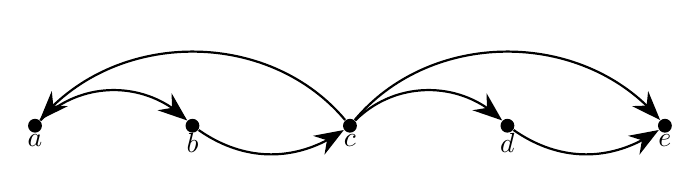
\begin{tikzpicture}[
        every node/.style={inner sep=0pt, minimum size=5pt},
        dot/.style={circle, fill=black},
        label style/.style={font=\itshape, yshift=-10pt},
        % এখানে scale=1.5 বাড়িয়ে arrowhead আরও বড় করতে পারবেন
        >={Stealth[scale=1.6]} 
    ]
        
        % 5টি ভার্টেক্স ডিফাইন করা হলো
        \node[dot, label={below:$a$}] (a) at (0,0) {};
        \node[dot, label={below:$b$}] (b) at (2,0) {};
        \node[dot, label={below:$c$}] (c) at (4,0) {};
        \node[dot, label={below:$d$}] (d) at (6,0) {};
        \node[dot, label={below:$e$}] (e) at (8,0) {};
        
        % image_d24201.png অনুযায়ী ডিরেক্টেড কার্ভড লাইনগুলো
        \path[->, thick]
            (a) edge[bend left=45] (b)
            (c) edge[bend right=50] (a)  % c থেকে a তে বড় ওপরের আর্ক
            (b) edge[bend right=35] (c)  % b থেকে c তে নিচের আর্ক
            (c) edge[bend left=45] (d)
            (c) edge[bend left=50] (e)   % c থেকে e তে বড় ওপরের আর্ক
            (d) edge[bend right=35] (e); % d থেকে e তে নিচের আর্ক

    \end{tikzpicture}
\end{center}

\mk{2+10} \yr{CSE 103 | L-1/T-2 | 2008--09}


%% 2016-17
\item Let $A = \{a, b, c\}$ and let $R$ be a binary relation on $A$ represented by the directed graph: $a \to b$, $b \to c$, $c \to a$.

\begin{center}
      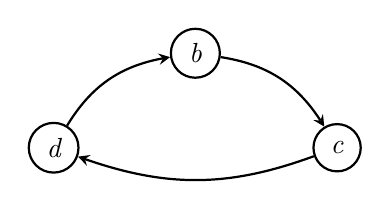
\begin{tikzpicture}[
        scale=1.5,
        % বৃত্তাকার নোডের সাধারণ স্টাইল
        every node/.style={circle, draw=black, thick, minimum size=0.6cm, font=\itshape},
        >=stealth, % তীরের মাথার স্টাইল সুন্দর করার জন্য
        thick
    ]

        % --- Nodes Positioning ---
        \node (d) at (0,0) {d};
        \node (b) at (1.2,0.8) {b};
        \node (c) at (2.4,0) {c};

        % --- Directed Curved Edges ---
        % d থেকে b তে উপর দিয়ে বাঁকানো তীর
        \draw[->] (d) to[bend left=25] (b);
        
        % b থেকে c তে ডান দিক দিয়ে বাঁকানো তীর
        \draw[->] (b) to[bend left=25] (c);
        
        % c থেকে d তে নিচ দিয়ে বাঁকানো তীর
        \draw[->] (c) to[bend left=20] (d);

    \end{tikzpicture}
\end{center}
\begin{enumerate}
  \item Show that $R^2 = R^{-1}$.
  \item Find the smallest integers $m$ and $n$ such that $m < n$ and $R^m = R^n$.
  \item Find $R^{99}$, $R^{100}$, and $R^{101}$. Explain how you arrived at your conclusion.
\end{enumerate}
\mk{3+4+5} \yr{CSE 103 | L-1/T-2 | 2006--07}

%% 2006-07
\item Let $R_1$ and $R_2$ be two binary relations on a set $A$. Determine whether the following statements are true or false. For each false statement, provide an example to show that it is false.
\begin{enumerate}
  \item If $R_1$ is antisymmetric, then $\overline{R_1}$ (complement) is also antisymmetric.
  \item If $R_1$ and $R_2$ are transitive, then $R_1 \,\Delta\, R_2$ (symmetric difference) is also transitive.
\end{enumerate}
\mk{3+3} \yr{CSE 103 | L-1/T-2 | 2006--07}

%% 2006-07
\item Let $R$ and $S$ be binary relations on a set $A$. Prove that if $R$ and $S$ are symmetric, so are $R \cap S$ and $R \cup S$.
\mk{8} \yr{CSE 103 | L-1/T-2 | 2006--07}


%% 2011-12
\end{enumerate}

%%──────────────────────────────────────────────────────────────────────
\subtopic{cB}{Equivalence Relations}
\label{sub:s4-equivalence}

\begin{enumerate}

%% Session: 2024-2025
\item Let $R$ be a relation on the set of integers, then determine if $R = \{(a,b) \mid a \equiv b \pmod{5}\}$ forms equivalence class on the set of integers or not. Find the partitions as well. Justify your answer.
\mk{12} \yr{CSE 103 | L-1/T-I | 2024--25}  

%% 2008-09
\item Let $R$ be a relation on the set of integers with modulus $m > 1$. Determine if $R = \{(a, b) \mid a \equiv b \pmod{m}\}$ is an equivalence relation on the set of integers or not. Justify your answer. (Hint: $m$ is a congruence modulo.)
\mk{6} \yr{CSE 103 | L-1/T-1 | 2023--24}

\item Define equivalence relation and partition. Give an example of an equivalence relation and explain how it partitions a set.
\mk{15} \yr{CSE 103 | L-1/T-2 | 2016--17}

  
%% 2012-13
\item What is an equivalence relation? Show that congruence modulo $n$ is an equivalence relation on $\mathbb{Z}$.
\mk{14} \yr{CSE 103 | L-1/T-2 | 2013--14}


%% 2023-24
\item We have a relation $R$ on the set of all bit strings of length three or more, consisting of all pairs $(x, y)$ such that $x$ and $y$ are bit strings that agree in their first and third bits.
\begin{enumerate}
  \item Show that the relation $R$ is an equivalence relation.
  \item What are the equivalence classes of $R$?
\end{enumerate}
\mk{7+8} \yr{CSE 103 | L-1/T-2 | 2012--13}

%% 2013-14
\item Let $R$ be an equivalence relation on a set $A$. Prove that the following statements are equivalent:
\begin{enumerate}
  \item $a\, R\, b$
  \item $[a] = [b]$
  \item $[a] \cap [b] \neq \emptyset$
\end{enumerate}
\mk{15} \yr{CSE 103 | L-1/T-2 | 2009--10, 2008--09}




%% 2009-10
\end{enumerate}

%%──────────────────────────────────────────────────────────────────────
\subtopic{cB}{Partial Ordered Sets}
\label{sub:s4-poset}

\begin{enumerate}


%% Session: 2024-2025
\item A server processes tasks numbered with the ids 2, 3, 4, 6, 9, 12, 18, 27, 48 and the task id numbering are divisible. Determine the topological sorting to process the tasks. (Show the steps.)
\mk{15} \yr{CSE 103 | L-1/T-I | 2024--25}

%% 2008-09
\item A biriyani shop's delivery person needs to deliver orders with IDs: $2, 3, 4, 6, 9, 12, 18, 27, 48$. The order IDs must be processed based on divisibility — for example, Order ID 4 can only be processed after Order ID 2 is processed, and so on. Determine the topological sorting plan to process the orders. Show all steps.
\mk{15} \yr{CSE 103 | L-1/T-1 | 2023--24}

%% 2022-23
\item What will be the maximal and minimal elements from the POSET of divisibility of $\{2, 4, 6, 9, 12, 18, 27, 36, 48, 60, 72\}$? What will be the topological sorted order?
\mk{15} \yr{CSE 103 | L-1/T-1 | 2022--23}

%% 2006-07
\item Let $R$ be the relation on a set $A = \{1, 2, 3\}$ where $R = \{(1,2),(1,3),(2,2),(2,3),(3,2)\}$. Answer the following:
\begin{enumerate}
  \item Find the reflexive closure of $R$.
  \item Find the symmetric closure of $R$.
  \item Using Warshall's algorithm, find the connectivity relation $R^*$.
\end{enumerate}
\mk{3+3+9} \yr{CSE 103 | L-1/T-2 | 2009--10}

%% 2023-24
\item \begin{enumerate}
  \item Find the symmetric closure of the relation $\neq$ on the set of integers.
  \item Find the transitive closure of the relation $>$ on the set of integers.
\end{enumerate}
\mk{2+2} \yr{CSE 103 | L-1/T-2 | 2008--09}

%% 2009-10
\item Let $A = \{a, b, c\}$ and let $\mathcal{P}(A)$ be the power set of $A$. Define the relation $R$ on $\mathcal{P}(A)$: for two subsets $S$ and $T$ of $A$, $(S, T) \in R$ if $S \subseteq T$. Draw a digraph for this relation. Determine its reflexivity, symmetry, antisymmetry, and transitivity.
\mk{9} \yr{CSE 103 | L-1/T-2 | 2006--07}

\end{enumerate}

%%──────────────────────────────────────────────────────────────────────
\subtopic{cB}{Hasse diagram}
\label{sub:s4-hasse}

\begin{enumerate}

%% Session: 2021-2022
\item A program contains six functions a, b, c, d, e, f. Function a takes input from b and d. Function b takes input from Function c. Function c and e do not need any input. Function $f$ takes input from Function a, and Function d takes input from both of the functions c and e. Find the Hasse diagram and the topological sorted order of the functions. Find the maximal and minimal elements of the diagram. (Show the steps.)
\mk{15} \yr{CSE 103 | L-1/T-I | 2021--22}  
  
%% Jan 2021
\item Find the Hasse diagram for the divisibility relation on the set $S = \{1, 5, 5^2, 5^3, 5^4, 5^5\}$. Find the topological sorted order of the elements, and the maximal and minimal elements. Show all steps.
\mk{20} \yr{CSE 103 | L-1/T-2 | Jan 2021}  

%% 2016-17
\item Find the Hasse diagram for the divisibility relation on the set $\{1, 3, 9, 27, 81, 243\}$. Show the steps. Find the maximal and minimal elements.
\mk{15} \yr{CSE 103 | L-1/T-2 | Jan 2020}

  %% Jan 2020
\item Draw the Hasse diagram for the partially ordered set (poset) $(A, R)$ where $A$ is the set of all subsets of $\{1, 2, 3\}$ and $R$ is the subset relation on $A$. Prove that if $(A, R)$ is a poset and $A$ is finite, then $A$ has a minimal element.
\mk{15} \yr{CSE 103 | L-1/T-2 | 2016--17}  


%% 2013-14
\item What is a partial ordering relation? Explain how we can construct a Hasse diagram for a partial ordering relation, with an illustrative example.
\mk{9} \yr{CSE 103 | L-1/T-2 | 2013--14}

%% 2013-14
\item The following courses have prerequisites as listed. Draw the Hasse diagram and determine in how many ways the courses can be taken sequentially.
\begin{center}
\begin{tabular}{ll}
\toprule
\textbf{Course} & \textbf{Prerequisites} \\\midrule
A & B, C \\
B & G \\
C & None \\
D & A, F \\
E & None \\
F & B, E \\
G & None \\\bottomrule
\end{tabular}
\end{center}
\mk{13} \yr{CSE 103 | L-1/T-2 | 2013--14}  


\item Draw the Hasse diagram for the partial ordering $\{(A, B) \mid A \subseteq B\}$ on the power set $\mathcal{P}(S)$ where $S = \{a, b, c\}$.
\mk{11} \yr{CSE 103 | L-1/T-2 | 2008--09}


%% 2008-09
\end{enumerate}

%% ══════════════════════════════════════════════════════════════════════
%%  PART III — NUMBER THEORY & COUNTING
%% ══════════════════════════════════════════════════════════════════════
\secdivider{Part III}{Number Theory \& Counting}{cC}{cC}

%% ── S5: Number Theory & Algebra ───────────────────────────────────────
\section{S5 --- Number Theory \& Algebra}
\label{sec:S5}
\markboth{S5 --- Number Theory \& Algebra}{}

%%──────────────────────────────────────────────────────────────────────
\subtopic{cC}{Divisibility \& Prime Numbers}
\label{sub:s5-divisibility}

\begin{enumerate}

%% Session: 2024-2025
\item Find out if every integer greater than 1 is either a prime number itself or can be expressed as a product of prime numbers in exactly one way, up to the order of the factors.
\mk{10} \yr{CSE 103 | L-1/T-I | 2024--25}

%% 2008-09
\item Prove or disprove that $2^{999} + 1$ is a prime number.
\mk{6} \yr{CSE 103 | L-1/T-1 | 2022--23}

%% 2022-23
\item Prove that $\forall$ natural number $n$, $n^2 + 3n + 2$ is composite.
\mk{6} \yr{CSE 103 | L-1/T-1 | 2022--23}

%% 2022-23
\item Justify that any integer $n > 1$ has a unique prime factorization (Fundamental Theorem of Arithmetic).
\mk{7} \yr{CSE 103 | L-1/T-1 | 2022--23}

\item Prove that there are infinitely many prime numbers.
\mk{7} \yr{CSE 103 | L-1/T-2 | 2015--16}

%% 2015-16
\item Prove that any positive integer has a unique prime factorization.
\mk{15} \yr{CSE 103 | L-1/T-2 | 2015--16}

%% 2011-12
\item Prove that for all integers $n \geq 0$, the number $9^{2n} - 64^n$ is divisible by 17.
\mk{12} \yr{CSE 103 | L-1/T-2 | 2012--13}  


%% 2022-23
\item Show that among any $n + 1$ positive integers not exceeding $2n$, there must be an integer that divides one of the other integers.
\mk{7} \yr{CSE 103 | L-1/T-2 | 2011--12}

%% 2012-13
\item Prove that there is no positive integer solution to $4a^3 + 2b^3 = c^3$.
\mk{10} \yr{CSE 103 | L-1/T-2 | 2009--10}

%% 2009-10
\item Prove that every integer greater than 1 is a product of primes.
\mk{10} \yr{CSE 103 | L-1/T-2 | 2009--10}

%% 2015-16
\item Prove that if 101 integers are selected from the set $\{1, 2, 3, \ldots, 200\}$, then there are two integers such that one divides the other.
\mk{10} \yr{CSE 103 | L-1/T-2 | 2008--09}

%% 2009-10
\end{enumerate}

%%──────────────────────────────────────────────────────────────────────
\subtopic{cC}{GCD, LCM \& Linear Combinations}
\label{sub:s5-gcdlcm}

\begin{enumerate}

%% 2023-24
\item Justify that, for all integers $x$ and $y$ where $x \neq 0$ and $y \neq 0$, if $d = \gcd(x, y)$, there exist integers $s$ and $t$ such that $d = xs + yt$ is the smallest positive linear combination.
\mk{15} \yr{CSE 103 | L-1/T-1 | 2023--24}

%% Session: 2021-2022
\item Prove that for all integers $x$ and $y$ where $x \neq 0$ and $y \neq 0$, if $d = \text{GCD}(x,y)$, there exist integers $s$ and $t$ such that $d = xs + yt$ expressed as a linear combination. (GCD means the greatest common divisor.)
\mk{12} \yr{CSE 103 | L-1/T-I | 2021--22}

\end{enumerate}

%%──────────────────────────────────────────────────────────────────────
\subtopic{cC}{Algebraic Structures}
\label{sub:s5-algebraic}

\begin{enumerate}


%% Session: 2024-2025
\item $M$ is set of all non singular matrices of order $n \times n$. Then, identify the algebraic structure for $M$ w.r.t matrix multiplication ($*$). Is $(M, *)$ an Abelian group? Justify your answer.
\mk{11} \yr{CSE 103 | L-1/T-I | 2024--25}

%% 2009-10
\item Determine the algebraic structure of $G = \{1, \omega, \omega^2\}$ under multiplication and justify your answer, where $1, \omega, \omega^2$ are the cube roots of unity.
\mk{10} \yr{CSE 103 | L-1/T-1 | 2023--24}

%% 2022-23
\item If $M$ is the set of all non-singular $n \times n$ matrices, determine if $(M, *)$ forms a group with respect to matrix multiplication $*$. Is $(M, *)$ an Abelian group? Justify your answer.
\mk{12+1} \yr{CSE 103 | L-1/T-1 | 2022--23}

%% Jan 2021
\item For the set $\mathbb{R}$, the addition ($+$) and multiplication ($*$) operations classify the algebraic structure $(\mathbb{R}, +, *)$. Show the steps of your findings — determine what algebraic structure this is (group, ring, field, etc.) and verify all axioms. If $\mathbb{R}$ is replaced by $\mathbb{R}^+$ (positive reals), what will happen to your structure and why?
\mk{15} \yr{CSE 103 | L-1/T-2 | Jan 2021}  

%% 2010-11
\item Find the properties of the algebraic structure $\langle S, * \rangle$ defined by the following Cayley table where $S = \{A, B, C, D, E, F\}$. Justify your answer. (Is it a group? Is it abelian? Identify the identity and inverses.)
\begin{center}
\begin{tabular}{c|cccccc}
$*$ & A & B & C & D & E & F \\\hline
A & A & B & C & D & E & F \\
B & B & A & E & F & C & D \\
C & C & F & A & E & D & B \\
D & D & E & F & A & B & C \\
E & E & D & B & C & F & A \\
F & F & C & D & B & A & E \\
\end{tabular}
\end{center}
\mk{14} \yr{CSE 103 | L-1/T-2 | Jan 2020}

\item What is an Abelian group? Show that any group $G$ is Abelian if and only if $(ab)^2 = a^2 b^2$ for all $a, b \in G$.
\mk{9} \yr{CSE 103 | L-1/T-2 | 2013--14}

%% 2013-14
\item Prove that for every finite group $G$, each group element appears exactly once in each row and each column of the group (Cayley) table.
\mk{10} \yr{CSE 103 | L-1/T-2 | 2013--14}

%% 2013-14
\item Show that the set of rigid motions (symmetries) of an equilateral triangle with the binary operation of composition is a nonabelian group.
\mk{16} \yr{CSE 103 | L-1/T-2 | 2013--14}

%% 2013-14
\item Let $S_5$ be the symmetric group on five symbols. Also, let
\[
  \alpha = \begin{pmatrix}1&2&3&4&5\\2&3&1&4&5\end{pmatrix} \quad \text{and} \quad
  \beta = \begin{pmatrix}1&2&3&4&5\\2&1&5&3&4\end{pmatrix}.
\]
Determine $\alpha\beta$, $\alpha^3$, $\beta^4$, $(\beta\alpha)^{-1}$, and $\beta^{-1}\alpha^{-1}$.
\mk{15} \yr{CSE 103 | L-1/T-2 | 2013--14}

%% 2013-14
\item What is a proper divisor of zero for the algebraic structure ``ring''? Prove that a finite integral domain is a field.
\mk{10} \yr{CSE 103 | L-1/T-2 | 2013--14}





%% 2023-24
\item Given $R = \{s, t, x, y\}$ with binary operations $\oplus$ and $\odot$ defined by the provided operation tables, determine whether $(R, \oplus, \odot)$ is a ring or not.

\begin{center}
  \begin{tabular}{cc}
        
        % --- প্রথম টেবিল (oplus operation) ---
        $\begin{array}{c|cccc}
            \oplus & s & t & x & y \\
            \hline
            s & y & x & s & t \\
            t & x & y & t & s \\
            x & s & t & x & y \\
            y & t & s & y & x 
        \end{array}$
        
        & \qquad\qquad\qquad % দুই টেবিলের মাঝখানের স্পেসিং
        
        % --- দ্বিতীয় টেবিল (odot operation) ---
        $\begin{array}{c|cccc}
            \odot & s & t & x & y \\
            \hline
            s & y & y & x & x \\
            t & y & y & x & x \\
            x & x & x & x & x \\
            y & x & x & x & x 
        \end{array}$

    \end{tabular}
\end{center}
\begin{enumerate}
  \item What is the inverse for $\oplus$?
  \item What is the zero element if $(R, \oplus, \odot)$ is a ring?
  \item Is $R$ commutative?
\end{enumerate}
\mk{10+2+2+3} \yr{CSE 103 | L-1/T-2 | 2013--14, 2010--11}



%% Jan 2020
\item Define the following algebraic structures and give examples for each:
\begin{enumerate}
  \item Group
  \item Ring
\end{enumerate}
\mk{10} \yr{CSE 103 | L-1/T-2 | 2009--10}




%% 2013-14
\end{enumerate}
%%──────────────────────────────────────────────────────────────────────
\subtopic{cC}{Modular Arithmetic}
\label{sub:s5-modular}

\begin{enumerate}

%% 2013-14
\item Write down an algorithm for computing $b^n \bmod m$. Using your algorithm, compute $3^{644} \bmod 645$.
\mk{20} \yr{CSE 103 | L-1/T-2 | 2015--16, 2013--14, 2011--12}

%% 2015-16
\item A man had 3 sons, 5 daughters, and 11 grandchildren. If he divides his money among only his sons, 2 taka is left; if among only his daughters, 3 taka is left; and if among all his children (sons and daughters), 9 taka is left. If he had no more than 1200 taka and no less than 1000 taka, what is the minimum amount he had? (Use the Chinese Remainder Theorem.)
\mk{20} \yr{CSE 103 | L-1/T-2 | 2015--16}  



%% 2011-12
\item Find the minimum $x$ that satisfies the following system of congruences:
\[
  x \equiv 2 \pmod{3}, \quad x \equiv 3 \pmod{5}, \quad x \equiv 1 \pmod{7}.
\]
\mk{15} \yr{CSE 103 | L-1/T-2 | 2013--14}



%% 2013-14
\item Solve the following linear congruence for $x$:
\[
  5x \equiv 8 \pmod{37}.
\]
\mk{10} \yr{CSE 103 | L-1/T-2 | 2013--14}


\item Show that among any group of five (not necessarily consecutive) integers, there are two with the same remainder when divided by 4.
\mk{7} \yr{CSE 103 | L-1/T-2 | 2012--13}



%% 2013-14
\item A man has 2 sons, 3 daughters, 5 grandsons, and 7 granddaughters. If he distributes his money among his sons, 1 taka is left; if distributed among daughters, 2 taka is left; if distributed among grandsons, 3 taka is left; and if distributed among only granddaughters, 4 taka is undistributed. What is the minimum amount of taka he can have? (Use the Chinese Remainder Theorem.)
\mk{15} \yr{CSE 103 | L-1/T-2 | 2011--12}



%% 2012-13
\end{enumerate}

\subtopic{cC}{Cryptography}
\label{sub:s5-cryptograpy}

\begin{enumerate}

%% Session: 2024-2025
\item What are the steps followed in a RSA cryptosystem?
\mk{10} \yr{CSE 103 | L-1/T-I | 2024--25}

%% 2010-11
\item We received the encrypted message $0981\;0461$. What is the decrypted message if it was encrypted using RSA with $p = 43$, $q = 59$, and $e = 13$?
\mk{20} \yr{CSE 103 | L-1/T-2 | 2015--16, 2013--14}  
  
%% 2011-12
\item Encrypt the word STOP using the RSA cryptosystem with $p = 43$, $q = 59$, $n = 43 \times 59 = 2537$, and public exponent $e = 13$, by replacing letters by their corresponding positions in the alphabet (A = 00, B = 01, \ldots, Z = 25).
\mk{20} \yr{CSE 103 | L-1/T-2 | 2011--12}

\item For the word ``cab'', an encryption function $E: \mathbb{Z}_{26} \to \mathbb{Z}_{26}$ is defined as $E(\theta) = (\alpha \cdot \theta + k) \bmod 26$ where $\alpha = 3$ and $k = 12$. Find the decryption function $D$ and show that after applying $D$ to the encrypted word, we recover ``cab'' again.
\mk{10} \yr{CSE 103 | L-1/T-2 | 2010--11}  

%% 2015-16
\end{enumerate}



%% ── S6: Counting & Combinatorics ──────────────────────────────────────
\section{S6 --- Counting \& Combinatorics}
\label{sec:S6}
\markboth{S6 --- Counting \& Combinatorics}{}

%%──────────────────────────────────────────────────────────────────────
\subtopic{cC}{Counting Principles \& Foundations}
\label{sub:s6-counting}

\begin{enumerate}

\item A standard deck of cards has 52 cards. There are 4 suits: hearts, diamonds, spades, and clubs. Each suit contains 13 cards (values): Aces, Kings, Queens, Jacks, and then Tens down to Twos. A hand consists of a sample of 5 cards drawn from the deck. Now determine the order of the hands mentioned in Table for Question 2(b) in terms of preference from higher to lower. A hand is preferred over another if the probability of having that hand is lower. Your final answer must be in the following format: $\text{hand name } X_1 > \text{hand name } X_2 > \dots > \text{hand name } X_5$. You must justify your answer.

\begin{longtable}{|l|p{10cm}|}
\hline
\textbf{Hand Name} & \textbf{Description} \\ \hline
\endfirsthead
\hline
\textbf{Hand Name} & \textbf{Description} \\ \hline
\endhead
\hline
\endfoot
\hline
\endlastfoot
One Pair & This hand has two cards of one value and the rest three cards having three distinct values which are different from the above value. So, this hand has the pattern AABCD, where A, B, C, and D are different values. \\ \hline
Two Pairs & This hand has two cards of one value, two cards of another value, and one card of a third value. So, this hand has the pattern AABBC where A, B, and C are different values. \\ \hline
Rainbow Hand & This is a hand with at least one card from each suit. \\ \hline
Full House & This is a hand with three cards of one value and two cards of another value. So, this hand has the pattern AAABB where A and B are different values. \\ \hline
Three of a Kind & This is a hand of three cards with the same value. This hand has the pattern AAABC, where A, B, and C are different values. \\ \hline
\end{longtable}
\mk{15} \yr{CSE 103 | L-1/T-I | 2024--25}

\item Country A wants to establish a balanced trade policy with Country B, where $n$ shipments of goods are exported from Country A to Country B, and $n$ shipments are imported from Country B to Country A over a fiscal year. However, at no point during the process can the cumulative number of imports from Country B exceed the cumulative number of exports to Country B.
\begin{enumerate}
  \item In how many distinct ways can Country A arrange these $n$ exports and $n$ imports?
  \item After one year, Country A wants to revise the trade policy. Country A now requires that, at least at one point during the fiscal year, the cumulative number of exports to Country B exceeds the cumulative number of imports from Country B. In how many distinct ways can Country A arrange these $n$ exports and $n$ imports?
\end{enumerate}
\mk{7+10} \yr{CSE 103 | L-1/T-1 | 2023--24}

\item Consider the following code snippet. Determine how many times the string \texttt{'Hello world'} will be printed.
\begin{lstlisting}
int i, j, k, p, n;
n = 10;
for (i = 1; i <= n; i++)
    for (j = 1; j <= i; j++)
        for (k = 1; k <= j; k++)
            for (p = 1; p <= k; p++)
                printf("Hello world\n");
\end{lstlisting}
\mk{10} \yr{CSE 103 | L-1/T-1 | 2023--24}

\item A standard deck of cards has 52 cards. There are 4 suits: hearts, diamonds, spades and clubs. There are 13 cards (i.e., values) in each suit. These are Aces, Kings, Queens, Jacks and then from Tens down to Twos. A hand consists of a sample of size 5 drawn from the deck. Now determine the order of the hands mentioned in Table 4.c in terms of preference from higher to lower. A hand is preferred over other if the probability of having that hand is lower. Your final answer must be in the following format: hand name $x_1$ > hand name $x_2$ > \dots > hand name $x_{6}$. You must justify your answer.

\begin{longtable}{|c|l|p{9cm}|}
\hline
\textbf{Item} & \textbf{Hand Name} & \textbf{Definition} \\ \hline
\endfirsthead
\hline
\textbf{Item} & \textbf{Hand Name} & \textbf{Definition} \\ \hline
\endhead
\hline
\endfoot
\hline
\endlastfoot
1 & one-pair & This hand has two cards of one value and the rest three cards having three distinct values which are different from the above value. So, this hand has the pattern AABCD, where A, B, C and D are different values. \\ \hline
2 & two-pair & This hand has two cards of one value, two cards of another value, and one card of a third value. So, this hand has the pattern AABBC where A, B and C are different values. \\ \hline
3 & royal flush & This consists of the Ten, Jack, Queen, King and Ace of one suit. \\ \hline
4 & three-of-a-kind & This is a hand of three cards with the same value (but, not a four-of-a-kind). This hand has the pattern AAABC where A, B and C are different values. \\ \hline
5 & four-of-a-kind & This is a hand of four cards with the same value. So, this hand has the pattern AAAAB where A and B are different values. \\ \hline
6 & full house & This is a hand with three cards of one value and two cards of another value. So, this hand has the pattern AAABB where A and B are different values. \\ \hline
\end{longtable}
\mk{24} \yr{CSE 103 | L-1/T-I | 2021--22}

\item After a tiresome online assignment in a sessional, all 30 of you went to the canteen to have some refreshing juice. The canteen offers following options: mango, orange, lemonade (2 types), banana and papaya. Deduce how many different ways you can select juice for all of you.
\mk{11} \yr{CSE 103 | L-1/T-I | 2021--22}

\item The following protocol has been proposed by your friend about a password system:
\begin{enumerate}
    \item Passwords will consist of 5 phrases separated by a space in between two consecutive phrases.
    \item Each phrase will be between 6 and 8 characters long. Characters can be digits or letters or one of the 7 special characters: !, \$, \^{}, \&, *, (, ).
    \item Each phrase must use at least one special character.
    \item The first phrase will start with a digit, the second one will start with a letter and the rest will start with a special character.
    \item The phrases are case sensitive, however, if the first character is a letter, then it must be a capital letter.
\end{enumerate}
You on the other hand, was planning to propose a rather simple protocol as follows:
\begin{enumerate}
    \item Password will be between 6 \& 8 characters long. Characters can be digit or letters, Letters are case sensitive.
    \item Passwords start with a letter.
\end{enumerate}
Analyze which one you will finally choose to have a better password system. Looking at both the proposals and your analysis, your genius little brother made a flying comment that your decision (following your analysis) would not change even if the phrases are only 3 characters long. Do you agree? You need to justify your answer.
\mk{15} \yr{CSE 103 | L-1/T-I | 2021--22}  

\item Derive a combinatorial proof for the following identity:
\[
  1 \times n + 2(n-1) + 3(n-2) + \cdots + (n-1) \times 2 + n \times 1 = \binom{n+2}{3}.
\]
\mk{10} \yr{CSE 103 | L-1/T-2 | 2020--21}

\item Consider all 5-letter words (need not be meaningful English words) formed from a subset $M$ of the English alphabet of size $L$, where $M$ consists of the first $L$ letters of the alphabet and $L = Y\%19 + 8$ ($Y$ being the last three digits of your student number). For each question below, first deduce a general formula in terms of $L$, then compute the result. If a question is not possible for a given $L$, identify the issue.
\begin{enumerate}
  \item How many such words are there in total?
  \item How many of these words contain no repeated letters?
  \item How many of these words start with the sub-word ``aha''?
  \item How many of these words either start with ``aha'' or end with ``bah'' or both?
  \item How many words containing no repeats also do not contain the sub-word ``bad''?
\end{enumerate}
\mk{15} \yr{CSE 103 | L-1/T-2 | Jan 2021}

\item Consider an 8-bit binary number $X$. The \textbf{weight} of $X$ is defined as the sum of its digits. For example, if $X = 01010101$, the weight of $X$ is 4.
\begin{enumerate}
  \item How many 8-bit binary numbers are there in total?
  \item How many 8-bit binary numbers have weight 5?
  \item Your genius brother claims that (ii) is equivalent to the question: ``How many subsets of the set $\{a, b, c, d, e, f, g, h\}$ contain exactly 5 elements?'' Do you agree? Justify your answer.
\end{enumerate}
\mk{12} \yr{CSE 103 | L-1/T-2 | Jan 2021}

\item IICT has set up the following rules for your BIIS password: a password is between 6 and 8 characters long, starts with a letter but contains digits or letters in other positions, and is case sensitive. Count the possible number of passwords.
\mk{8} \yr{CSE 103 | L-1/T-2 | Jan 2021}

\item How many 4-digit numbers are there with at least one digit equal to 7, when leading zeros are not allowed?
\mk{8} \yr{CSE 103 | L-1/T-2 | Jan 2020}

\item How many 4-digit numbers divisible by 11 are \textbf{not} palindromes? (A palindromic number remains the same when its digits are reversed, e.g., 1221.)
\mk{14} \yr{CSE 103 | L-1/T-2 | Jan 2020}

\item Suppose each banknote has a code number of length 8 consisting of a 2-letter code followed by a 6-digit serial number (the serial number may contain leading zeros). A note is called \textbf{defective} if there are repeated letters or some digit appears more than once in the code. How common are non-defective notes? (i.e., how many non-defective codes exist?)
\mk{8} \yr{CSE 103 | L-1/T-2 | Jan 2020}

\item Find the relationship between Stirling numbers of the second kind and onto functions in the context of finding two-factor and three-factor factorizations greater than 1 for the number 156009.
\mk{12} \yr{CSE 103 | L-1/T-2 | Jan 2020}

\item Your teacher gave your friend a counting problem, and his result is $\binom{10}{4}\binom{6}{3}\binom{3}{2}\binom{1}{1}$. However, his lab partner came up with $\binom{10}{1}\binom{9}{2}\binom{7}{3}\binom{4}{4}$. The teacher gave both of them full marks. Propose a scenario and provide a combinatorial argument explaining how the two expressions are counting the same thing.
\mk{5} \yr{CSE 103 | L-1/T-2 | 2020--21}

\item All of your classmates in your section went to a restaurant to dine. Since you are on a budget, you decided to choose one of the set menus. There are a total of five different set menus having the least cost, which is however higher than your budget. The owner of the restaurant, a math enthusiast, gave you a lifeline: ``If you can count the number of different ways to select set menus for you and your classmates (one menu per person), I will offer you `Buy 1 Get 1 Free'.'' Analyse the scenario and determine the count, assuming your section has $n$ students including yourself.
\mk{15} \yr{CSE 103 | L-1/T-2 | 2020--21}

\item In how many ways can Mr.\ Rafiq distribute ten distinct books to his ten students (one book for each) and then collect and redistribute the books so that each student has the opportunity to read two different books?
\mk{7} \yr{CSE 103 | L-1/T-2 | 2016--17}

\item How many bit strings of length 5 contain more 0s than 1s?
\mk{7} \yr{CSE 103 | L-1/T-2 | 2015--16}

\item Find the value of ``sum'' after the following program segment is executed (variables are integers). Show the counting in detail.
\begin{lstlisting}
increment := 0
sum := 0
for i := 1 to 10 do
  for j := 1 to i do
    for k := 1 to j do
    begin
      increment := increment + 1
      sum := sum + increment
    end
\end{lstlisting}
\mk{12} \yr{CSE 103 | L-1/T-2 | 2013--14}

\item How many distinct paths are there from $(-1, 2, 0)$ to $(1, 3, 7)$ in Euclidean three-space if each move is one of the following types?
\begin{itemize}
  \item (H): $(x,y,z) \to (x+1,y,z)$
  \item (V): $(x,y,z) \to (x,y+1,z)$
  \item (A): $(x,y,z) \to (x,y,z+1)$
\end{itemize}
\mk{13} \yr{CSE 103 | L-1/T-2 | 2013--14} 

\item Each user on a computer system has a password configuration consisting of uppercase letters or digits. Find the number of possible passwords in the following configurations:
\begin{enumerate}
  \item The password is 5 to 8 characters long and must contain at least two digits. \mk{7} \yr{CSE 103 | L-1/T-2 | 2012--13}
  \item The password is 6 to 8 characters long and must contain at least one digit. \mk{8} \yr{CSE 103 | L-1/T-2 | 2009--10}
\end{enumerate}

\item A palindrome is a string whose reversal is identical to the string. How many bit strings of length $n$ are palindromes?
\mk{7} \yr{CSE 103 | L-1/T-2 | 2009--10}

\item How many ways are there to assign five different jobs to four different employees if every employee is assigned at least one job?
\mk{10} \yr{CSE 103 | L-1/T-2 | 2009--10}

\item There are 38 different time periods in a week during which classes at a university can be scheduled. If there are 677 different classes in a week, how many different rooms will be needed?
\mk{5} \yr{CSE 103 | L-1/T-2 | 2009--10}

\end{enumerate}

%%──────────────────────────────────────────────────────────────────────
\subtopic{cC}{Combinations, Permutations \& Stars-and-Bars}
\label{sub:s6-combinations}

\begin{enumerate}

\item There are 30 books arranged in a row on a shelf. Evaluate how many ways there are to choose 5 of these books such that between any two selected books, there are at least 3 other books that are not selected. In other words, if one book is selected, then the next three books to its right must not be selected.
\mk{10} \yr{CSE 103 | L-1/T-I | 2024--25}  

\item Determine the total number of distinct configurations for placing chess pieces on a standard chessboard under the following independent restrictions:
\begin{enumerate}
  \item Placing one rook, one knight, and one pawn so that they do not share a row or column. \mk{15} \yr{CSE 103 | L-1/T-1 | 2023--24}
  \item Placing three identical pawns so that they do not share a row or column. \mk{15} \yr{CSE 103 | L-1/T-1 | 2023--24}
\end{enumerate}

\item In a lab with 25 identical computers, 5 teams are working on their term projects. Each team must be assigned at least two computers, and all 25 computers must be distributed among the teams. How many different ways can the computers be assigned to these teams?
\mk{10} \yr{CSE 103 | L-1/T-1 | 2023--24}

\item The juice corner of the ECE café offers juice of 5 fruits: apple, mango, lemon, papaya, and pineapple. For each fruit you have two options: with sugar or without sugar. After a tiresome class test, all 180 CSE 103 course students went to the juice corner to get refreshed. Knowing that these are the students of CSE 103, the owner (who is a math enthusiast) offered a 50\% discount if the students could determine how many different ways the juice can be selected for all of them. Can you get the 50\% discount? Count using a suitable mapping and provide a detailed explanation.
\mk{12} \yr{CSE 103 | L-1/T-1 | 2022--23}

\item There are 20 books arranged in a row on a shelf. How many ways are there to choose 6 of these books so that no two adjacent books are selected?
\mk{10} \yr{CSE 103 | L-1/T-2 | 2017--18}

\item Count the number of integer solutions to $x_1 + x_2 + x_3 + x_4 + x_5 + x_6 \leq 20$, where $x_1 \geq 1$ and $x_2, x_3, x_4, x_5, x_6 \geq 2$.
\mk{10} \yr{CSE 103 | L-1/T-2 | 2017--18}

\item Is there any connection between the previous two questions (books on shelf and integer solutions)? Explain.
\mk{5} \yr{CSE 103 | L-1/T-2 | 2017--18}

\item There are a total of 12 undergraduate-degree-offering departments in BUET. Each department is led by a Head of Department, and the undergraduate program is managed by a BUGS (Board of Undergraduate Studies) Secretary. A three-member committee has been formed by the Academic Council of BUET to evaluate and monitor undergraduate programs. The committee will comprise a Chairman (one of the Heads of the undergraduate-degree-offering departments) and two other members taken from the BUGS Secretaries. However, from one department you cannot have more than one member in the committee. Count the number of ways to form the committee.
\mk{7} \yr{CSE 103 | L-1/T-2 | 2017--18}

\item Find the number of integer solutions to the following algebraic equations under upper/lower bounds:
\begin{enumerate}
  \item $x_1 + x_2 + x_3 + x_4 = 18$ where $x_i$ are non-negative integers such that $x_i \leq 7$ for all $1 \leq i \leq 4$. \mk{8} \yr{CSE 103 | L-1/T-2 | 2016--17}
  \item $x_1 + x_2 + x_3 = 13$ where $x_1, x_2$, and $x_3$ are non-negative integers less than 6. \mk{13} \yr{CSE 103 | L-1/T-2 | 2015--16}
  \item $x_1 + x_2 + x_3 + x_4 = 15$, where $x_1, x_2, x_3, x_4$ are non-negative integers such that $x_1 \leq 3$, $x_2 \leq 4$, and $x_4 > 3$. \mk{10} \yr{CSE 103 | L-1/T-2 | 2009--10}
  \item $a + b + c + d = 40$, where $a, b, c, d$ are all non-negative integers satisfying $a > 3$ and $c > 15$. \mk{12} \yr{CSE 103 | L-1/T-2 | 2012--13}
\end{enumerate}

\item A chemist who has five assistants is engaged in a research project that calls for nine compounds that must be synthesized. In how many ways can the chemist assign these syntheses to the five assistants so that each assistant is working on at least one synthesis?
\mk{7} \yr{CSE 103 | L-1/T-2 | 2016--17}

\item In how many ways can a photographer at a wedding arrange six people in a row, including the bride and groom, if the bride is positioned somewhere to the left of the groom?
\mk{12} \yr{CSE 103 | L-1/T-2 | 2015--16}

\item How many ways can you distribute 12 identical apples and 10 identical mangoes to 4 people so that each person gets at least one apple and one mango?
\mk{12} \yr{CSE 103 | L-1/T-2 | 2012--13}

\item For integers $n, r$ with $n \geq r \geq 1$, prove that
\[
  \binom{n+1}{r} = \binom{n}{r} + \binom{n}{r-1}.
\]
\mk{7} \yr{CSE 103 | L-1/T-2 | 2013--14}  

\item Find the value of $\displaystyle\sum_{i=0}^{100} \binom{100}{i} (-2)^i$.
\mk{7} \yr{CSE 103 | L-1/T-2 | 2012--13}

\item A teacher starts each year with 3 jokes. Over 12 years the teacher never repeated the same triple of jokes. What is the smallest number of jokes the teacher must know for this to be possible?
\mk{6} \yr{CSE 103 | L-1/T-2 | 2006--07}

\item Given a set of objects with (weight, profit) pairs: $(1,2), (1,3), (2,3), (2,5), (3,4), (4,7)\\, (5,8), (6,9), (7,11)$. Choose objects greedily for a knapsack of capacity $W = 12$ so that the maximum profit is earned. Objects can be chosen fractionally.
\mk{10} \yr{CSE 103 | L-1/T-2 | 2017--18}

\end{enumerate}

%%──────────────────────────────────────────────────────────────────────
\subtopic{cC}{Pigeonhole Principle \& Derangements}
\label{sub:s6-pigeonhole}

\begin{enumerate}

\item Over a given tracking period (consecutive days or matches), establish that there exists a specific consecutive window during which a precise target value of items/actions is achieved. (General Framework: Let $a_i$ be the cumulative items where at least one occurs per day, bounded globally).
\mk{12} \yr{CSE 103 | L-1/T-I | 2024--25} \variant{Jan 2020, 2016--17, 2013--14, 2009--10, 2006--07}

\item Prove the classic Ramsey Theorem condition $R(3,3) = 6$ using the Pigeonhole Principle framework: every collection of 6 entities (people, students) must include either a mutual subgroup of 3 related members (friends, club, same ICPC team) or a subgroup of 3 completely independent strangers.
\mk{15} \yr{CSE 103 | L-1/T-1 | 2022--23} \variant{2017--18, 2013--14, 2009--10}

\item If there is a square space where each side is $s$ units, justify the maximum distance metric between multiple arbitrary internal points:
\begin{enumerate}
  \item Among 5 points placed in a square of side 1 ft, at least two points have a distance apart of less than $\dfrac{1}{\sqrt{2}}$ ft. \mk{10} \yr{CSE 103 | L-1/T-1 | 2023--24}
  \item Among 5 points placed in a square of side 2 units, prove that at least two of them are within a distance of at most $\sqrt{2}$ from each other. \mk{5} \yr{CSE 103 | L-1/T-2 | 2020--21}
\end{enumerate}

\item In your C/C++ sessional, you have been given the following assignment (Assignment A) which will be evaluated automatically using an online judge. \\[6pt]
\textbf{Assignment A: Subset Sum}\\
You will be given ninety 25-digit numbers. You will need to check whether there exist two different subsets with the same sum. Your input will be ninety 25-digit numbers, one per line, and you will have to output ``Yes'' if there exist two different subsets with the same sum, or ``No'' otherwise. Your solution must be as efficient as possible.\\[4pt]
Your genius little brother suggests writing a simple code that outputs ``Yes'' for all inputs without checking anything. Do you think his solution is always correct? Justify your answer.
\mk{10} \yr{CSE 103 | L-1/T-1 | 2022--23}

\item How many numbers must be selected from the set $\{1, 3, 5, 7, 9, 11, 13, 15\}$ to guarantee that:
\begin{enumerate}
    \item at least two pairs of these numbers add up to 16?
    \item at least one pair of these numbers add up to 8?
\end{enumerate}
\mk{8} \yr{CSE 103 | L-1/T-I | 2021--22}

\item A workshop on Network Security has 40 participants. All participants are in the age range from 17 to 34 years (inclusive). Determine whether there are at least $x$ participants of the same age. What may be the maximum value of $x$? Explain your answer.
\mk{10} \yr{CSE 103 | L-1/T-2 | Jan 2021}

\item Your team is playing the final match of a 5-a-side football tournament and drew the match with the opponent team. The winner now will be decided through a penalty shootout where $2$ of the players will be selected from each team who will take part in the penalty shootout as per the by-laws of the tournament. As the adviser you now need to decide the two penalty shooters from your team. Your genius little brother proposes: ``Choose two players having jersey numbers such that their difference is divisible by $4$.'' According to Pigeon Hole Principle, derive a proof that you indeed will get one such pair.
\mk{10} \yr{CSE 103 | L-1/T-2 | 2020--21}

\item Prove via the generalized pigeonhole principle that among $N$ components/people in a connected network or system, there is always a pair of nodes containing the exact same number of handshakes/degree connections.
\mk{9} \yr{CSE 103 | L-1/T-2 | 2010--11} \variant{2008--09, 2006--07}

\item Prove using the pigeonhole principle that for any graph $G = (V, E)$ where $|V| = n$, if vertex $u \in V$ is connected to vertex $w \in V$, there exists a simple path from $u$ to $w$ having no more than $n$ vertices.
\mk{10} \yr{CSE 103 | L-1/T-2 | 2017--18}

\item Prove that at least four of any 37 days must fall on the same month in a year.
\mk{7} \yr{CSE 103 | L-1/T-2 | 2017--18}

\item Any subset of size 6 from the set $S = \{1, 2, 3, \ldots, 9\}$ must contain two elements whose sum is 10. Prove it.
\mk{8} \yr{CSE 103 | L-1/T-2 | 2016--17}

\item Prove that every sequence of $n^2 + 1$ distinct real numbers contains a subsequence of length $n + 1$ that is either strictly increasing or strictly decreasing.
\mk{12} \yr{CSE 103 | L-1/T-2 | 2011--12}

\item Prove that any collection of eight distinct integers contains distinct integers $x$ and $y$ such that $x - y$ is a multiple of 7.
\mk{10} \yr{CSE 103 | L-1/T-2 | 2010--11}

\item Prove that if seven distinct numbers are selected from $\{1,2, \dots, 11\}$, then some two of these numbers sum to 12.
\mk{10} \yr{CSE 103 | L-1/T-2 | 2009--10}

\item State and prove the generalized pigeonhole principle.
\mk{5} \yr{CSE 103 | L-1/T-2 | 2009--10}

\item Show that there must be at least two people in Dhaka city with the same number of hairs on their heads. A typical head has around 150,000 hairs. Election commission statistics show that there live more than 1,00,000,000 people in Dhaka city.
\mk{6} \yr{CSE 103 | L-1/T-2 | 2008--09}

\item How many students in a discrete math course must be enrolled to ensure that 6 students get the same grade? Note that the available grades are: A, B, C, D, and F.
\mk{6} \yr{CSE 103 | L-1/T-2 | 2006--07}

\item General Distribution Principles (Pigeonhole Mapping):
\begin{enumerate}
  \item Given 6 physics books, 17 chemistry books, 8 mathematics books, 20 history books, and 12 english literature books, how many of these books must we select to ensure that we have 15 books dealing with the same subject? \mk{10} \yr{CSE 103 | L-1/T-2 | 2008--09}
  \item A box contains 10 French books, 20 Spanish books, 8 German books, 15 Russian books, and 25 Italian books. How many books must we choose to ensure that we have 12 books in the same language? \mk{7} \yr{CSE 103 | L-1/T-2 | 2006--07}
\end{enumerate}

\item Applications of Derangements ($D_n$ Framework):
\begin{enumerate}
  \item In how many ways can the digits 1, 2, 3, 4, 5, 6, 7, 8 be arranged so that no even digit is in its original position? \mk{13} \yr{CSE 103 | L-1/T-2 | 2015--16}
  \item A robotic machine inserts letters into envelopes. What is the probability that in a group of 100 letters: (i) No letter is put into correct envelope? (ii) Exactly 1 letter is correct? (iii) Exactly 98 letters are correct? \mk{15} \yr{CSE 103 | L-1/T-2 | 2013--14}
  \item A new employee checks the hats of $n$ people at a restaurant, randomly giving them back. What is the probability that exactly one person gets their correct hat? \mk{12.5} \yr{CSE 103 | L-1/T-2 | 2016--17, 2012--13}
  \item Find the number of derangements of $n$ objects. Derive the formula and simplify. \mk{10} \yr{CSE 103 | L-1/T-2 | 2011--12}
\end{enumerate}

%% 2008-09
\item Prove that any collection of 6 people includes a club of 3 people or a group of 3 strangers. (In a \textbf{club}, every pair of people has met; in a \textbf{group of strangers}, no pair has met.)
\mk{10} \yr{CSE 103 | L-1/T-2 | 2009--10}  

\end{enumerate}

%%──────────────────────────────────────────────────────────────────────
\subtopic{cC}{Inclusion-Exclusion Principle}
\label{sub:s11-inclusion}

\begin{enumerate}

%% 2020-21
\item Consider that 200 candidates were interviewed for a position at a call center. Of them, 100 had a two-wheeler, 70 had a credit card, and 140 had a mobile phone. 40 had both a two-wheeler and a credit card; 30 had both a credit card and a mobile phone; 60 had both a two-wheeler and a mobile phone; and 10 had all three. Using set theory, find how many candidates had none of the three?
\mk{10} \yr{CSE 103 | L-1/T-2 | 2020--21}

\item In how many ways can one arrange the letters of the word CORRESPONDENTS so that:
\begin{enumerate}
  \item There are exactly two pairs of consecutive identical letters.
  \item There are at least three pairs of consecutive identical letters.
\end{enumerate}
\mk{8+8} \yr{CSE 103 | L-1/T-2 | 2016--17}

\item Given $|A| = 30$, $|B| = 42$, $|A \cap B| = 15$, $|A \cap C| = 14$, $|B \cap C| = 13$, $|A \cup B \cup C| = 80$. What could be the maximum value of $|C|$?
\mk{7} \yr{CSE 103 | L-1/T-2 | 2017--18}   

\item For $1 \leq m \leq t$, the number of elements in $S$ that satisfy exactly $m$ of the conditions $c_1, c_2, \ldots, c_t$ is given by:
\[
  S_m - \binom{m+1}{1}S_{m+1} + \binom{m+2}{2}S_{m+2} - \cdots + (-1)^{t-m}\binom{t}{t-m}S_t
\]
where $S_n$ denotes the total number of elements satisfying at least $n$ of the conditions. Prove the above statement.
\mk{12} \yr{CSE 103 | L-1/T-2 | 2013--14}

\item How many integers between 1 and 1000 are divisible by 4, 5, or 13 but not divisible by 10?
\mk{11} \yr{CSE 103 | L-1/T-2 | 2012--13}

\item Of 1000 applicants for a mountain-climbing trip in the Himalayas, 450 get altitude sickness, 622 are not in good enough shape, and 30 have allergies. An applicant qualifies if and only if they do not get altitude sickness, are in good shape, and do not have allergies. If there are 111 applicants who get altitude sickness and are not in good enough shape, 14 who get altitude sickness and have allergies, 18 who are not in good enough shape and have allergies, and 9 who get altitude sickness, are not in good enough shape, and have allergies, how many applicants qualify?
\mk{15} \yr{CSE 103 | L-1/T-2 | 2012--13}

\item Let $A_1, A_2, \ldots, A_n$ be finite sets. Prove that
\[
  |A_1 \cup A_2 \cup \cdots \cup A_n| = \sum_{1 \leq i \leq n}|A_i| - \sum_{1 \leq i < j \leq n}|A_i \cap A_j| + \cdots + (-1)^{n+1}|A_1 \cap A_2 \cap \cdots \cap A_n|.
\]
\mk{8} \yr{CSE 103 | L-1/T-2 | 2011--12}

\item If a set $S$ has $N$ elements, and $\bar{N}$ denotes the number of elements satisfying none of the conditions $c_i$ for $1 \leq i \leq t$, find/prove the principle of inclusion-exclusion theorem representation:
\[
  \bar{N} = N - \sum_{1 \leq i \leq t} N(c_i) + \sum_{1 \leq i < j \leq t} N(c_i c_j) - \sum_{1 \leq i < j < k \leq t} N(c_i c_j c_k) + \cdots + (-1)^t N(c_1 c_2 \cdots c_t)
\]
\mk{12} \yr{CSE 103 | L-1/T-2 | 2016--17, 2010--11}

\item Determine the number of positive integers $n$ where $1 \leq n \leq 100$ and $n$ is neither divisible by 2 nor 5, but $n$ is divisible by 3.
\mk{8} \yr{CSE 103 | L-1/T-2 | 2010--11}

\item In how many ways can the 26 letters of the alphabet be permuted so that none of the patterns ``car'', ``dog'', ``byte'', ``funs'' occurs?
\mk{7} \yr{CSE 103 | L-1/T-2 | 2010--11}

\end{enumerate}



\secdivider{Part IV}{Recurrences \& Probability}{cD}{cD}


\section{S7 --- Recurrence Relations}
\label{sec:S7}
\markboth{S7 --- Recurrence Relations}{}

%%──────────────────────────────────────────────────────────────────────
\subtopic{cD}{Formulation \& Applications}
\label{sub:s7-recurrence-formulation}

\begin{enumerate}

\item A newborn pair of rabbits (one male and one female) is placed on an island. Rabbits mature after one month and start reproducing from the second month onward. A mature rabbit pair produces two new pairs (each pair contains one male and one female) each month. Let $R_n$, $B_n$, $M_n$ represent the total number of rabbit pairs, the number of newborn rabbit pairs, and the number of mature rabbit pairs at the end of month $n$, respectively.
\begin{enumerate}
  \item Derive the recurrence relation for $R_n$ (the total number of rabbit pairs at the end of month $n$).
  \item Solve the recurrence relation for $R_n$.
\end{enumerate}
\mk{18} \yr{CSE 103 | L-1/T-1 | 2023--24}

\item You are working with a population of rabbits. Each mature rabbit pair gives birth to two new pairs each month. Each pair becomes mature after two months. Determine the following quantities using a recursive approach:
\begin{enumerate}
  \item Number of newborn pairs at the end of month $n$, $w_n$.
  \item Number of mature pairs at the end of month $n$, $m_n$.
\end{enumerate}
Also, mention the order of each recurrence relation.
\mk{12} \yr{CSE 103 | L-1/T-1 | 2022--23}

\item Consider the set of strings made of the characters from $\{a, b, c, d\}$. We want to discard the strings that contain the pattern "aa". Therefore, "aab", "caaad", "aaaa" etc. are invalid strings. Formulate a recurrence relation to find the number of valid strings of length $n$. Finally, solve the recurrence relation.
\mk{17} \yr{CSE 103 | L-1/T-I | 2021--22}  

\item Find a recurrence relation and give initial conditions for the number of bit strings of length $n$ that do not contain three consecutive 0s. (Note: Varied extensions ask for the solution or the specific count for length seven).
\mk{15} \yr{CSE 103 | L-1/T-2 | 2012--13} \variant{2011--12, 2009--10}

\item For each integer $n \geq 0$, let $x_n$ denote the number of bit strings of length $n$ that do not contain the bit pattern 111. Find the recurrence relation for $x_0, x_1, x_2, \ldots$
\mk{12} \yr{CSE 103 | L-1/T-2 | Jan 2021}  

\item An alphabet set $A$ consists of three numeric characters $\{1, 2, 3\}$ and five alphabetic characters $\{p, q, r, s, t\}$. Deduce and solve the recurrence relation for the number of words of length $k$ (using alphabet set $A$) where there are no two consecutive alphabetic characters (whether identical or distinct).
\mk{10} \yr{CSE 103 | L-1/T-2 | Jan 2020}

\item A \textbf{palindrome} is a sequence of characters that reads the same backward as forward. For example, 5, 070, and 9449 are palindromes, whereas 132 and 6436 are not. Find a recurrence relation and give initial conditions for the number of strings of decimal digits that are palindromes.
\mk{15} \yr{CSE 103 | L-1/T-2 | 2016--17}

\item Find the recurrence relation satisfied by $R_n$, where $R_n$ is the number of regions that a plane is divided into by $n$ lines, if no two of the lines are parallel and no three of the lines pass through the same point.
\mk{15} \yr{CSE 103 | L-1/T-2 | 2016--17}

\item A string that contains only 0s, 1s, and 2s is called a \textbf{ternary string}. Find a recurrence relation for the number of ternary strings of length $n$ that do not contain two consecutive symbols that are the same. Explain how you obtain your answer. What are the initial conditions?
\mk{10} \yr{CSE 103 | L-1/T-2 | 2015--16}

\item Find a recurrence relation for the number of ways to climb $n$ stairs if the person climbing can take one, two, or three stairs at a time. Explain how you obtain your answer. What are the initial conditions?
\mk{7} \yr{CSE 103 | L-1/T-2 | 2015--16}

\item For $b \in \mathbb{R}^+$, set up and solve the appropriate recurrence relation to find the determinant $D_n$ of an $n \times n$ tridiagonal matrix whose main diagonal and the two adjacent diagonals all have value $b$ (all other entries are 0).
\begin{center}
  \[
  D_n = \begin{vmatrix}
  b & b & 0 & 0 & 0 & \dots & 0 \\
  b & b & b & 0 & 0 & \dots & 0 \\
  0 & b & b & b & 0 & \dots & 0 \\
  \vdots & & \ddots & \ddots & \ddots & & \vdots \\
  0 & \dots & 0 & b & b & b & 0 \\
  0 & \dots & \dots & 0 & b & b & b \\
  0 & \dots & \dots & \dots & 0 & b & b 
  \end{vmatrix}
  \]
\end{center}
\mk{13} \yr{CSE 103 | L-1/T-2 | 2013--14, 2010--11}   

\item In a communication channel, words of length $n$ are to be transmitted using the symbol set $\{a, b, c\}$ with the condition that no word will contain two consecutive `a' symbols. Find the number of allowed words using a recursive approach.
\mk{10} \yr{CSE 103 | L-1/T-2 | 2013--14}  

\item Write down the recursive definition of the sequence $a_1, a_2, \ldots, a_{n-1}, a_n, a_{n+1}, \ldots$ given that for any $n$, the value of $a_n = 6n$.
\mk{7.5} \yr{CSE 103 | L-1/T-2 | 2012--13}

\item How can you express the number of comparisons used by merge sort using a recurrence relation?
\mk{5} \yr{CSE 103 | L-1/T-2 | 2011--12}

\item To sort $n$ numbers using bubble sort, find the value of the number of comparisons $a_n$. What type of recurrence is $a_n$?
\mk{5} \yr{CSE 103 | L-1/T-2 | 2010--11}

\item For $n \geq 0$, if $S = \{1, 2, 3, \ldots, n\}$, let $a_n$ denote the number of subsets of $S$ that contain no two consecutive integers. Show that $a_n = F_{n+2}$ for $n \geq 0$, where $F_{n+2}$ is the $(n+2)$-th Fibonacci number. (Derive the recurrence relation only.)
\mk{5} \yr{CSE 103 | L-1/T-2 | 2010--11}

\item What is the minimum number of moves needed to solve the ``Towers of Hanoi'' problem for $n$ disks and three poles? Derive the recurrence relation and solve it.
\mk{6} \yr{CSE 103 | L-1/T-2 | 2010--11}

\end{enumerate}


%%──────────────────────────────────────────────────────────────────────
\subtopic{cD}{Solution Methods \& Theorems}
\label{sub:s7-recurrence-solving}

\begin{enumerate}

\item Find the solution of the following recurrence relation:
\[
  r_n = r_{n-1} + 2r_{n-2} + 1, \quad r_0 = 0,\; r_1 = 1.
\]
\mk{15} \yr{CSE 103 | L-1/T-1 | 2022--23}

\item A sequence $1, t, t^2, t^3, t^4, \ldots, t^n$ with $t \neq 0$ satisfies the recurrence relation $a_k = a_{k-1} + 6a_{k-2}$ with initial conditions $a_0 = 0$, $a_1 = 3$ for all integers $k \geq 2$. Find the explicit formula for the sequence.
\mk{13} \yr{CSE 103 | L-1/T-2 | Jan 2021}

\item Show that the Fibonacci sequence is a second-order homogeneous recurrence relation and find its closed-form/unique solution using the Distinct-Roots Theorem.
\mk{15} \yr{CSE 103 | L-1/T-2 | 2020--21} \variant{2017--18, 2010--11}

\item Present the \textbf{distinct root theorem} and \textbf{single root theorem} in the context of second-order recurrence relations.
\mk{6} \yr{CSE 103 | L-1/T-2 | 2017--18}

\item Solve the recurrence relation $a_n = 6a_{n-1} - 12a_{n-2} + 8a_{n-3}$ with $a_0 = -5$, $a_1 = 4$, and $a_2 = 88$.
\mk{8} \yr{CSE 103 | L-1/T-2 | 2015--16}

\item Find the unique solution of the recurrence relation: $6a_n - 7a_{n-1} = 0$, $n \geq 1$, $a_3 = 343$.
\mk{9} \yr{CSE 103 | L-1/T-2 | 2013--14}  

\item Solve the recurrence relation: $a_n = 6a_{n-1} - 9a_{n-2}$ for $n \geq 2$, with $a_0 = 2$, $a_1 = 9$.
\mk{10} \yr{CSE 103 | L-1/T-2 | 2012--13}

\item Let $c_1$ and $c_2$ be real numbers. Suppose that $r^2 - c_1 r - c_2 = 0$ has two distinct roots $r_1$ and $r_2$. Show that the sequence $\{a_n\}$ is a solution of the recurrence relation $a_n = c_1 a_{n-1} + c_2 a_{n-2}$ if and only if $a_n = \alpha_1 r_1^n + \alpha_2 r_2^n$ for $n = 0, 1, 2, \ldots$, where $\alpha_1$ and $\alpha_2$ are constants.
\mk{15} \yr{CSE 103 | L-1/T-2 | 2011--12}

\item Find the solution to the recurrence relation
\[
  a_n = 3a_{n-1} - 3a_{n-2} + 3a_{n-3}
\]
with initial conditions $a_0 = 1$, $a_1 = 2$, $a_2 = 3$.
\mk{10} \yr{CSE 103 | L-1/T-2 | 2009--10}

\end{enumerate}

%%──────────────────────────────────────────────────────────────────────
\subtopic{cD}{Generating Functions}
\label{sub:s7-genfunc}

\begin{enumerate}

\item Howard learned about the recurrence relation for the Tower of Hanoi problem during his engineering studies at MIT. Sheldon mocks Howard for his engineering degree and decides to test his skills with a challenging problem. He told Howard that he needed to demonstrate the recurrence relation for the minimum number of moves required for the Tower of Hanoi problem, adding a constraint: direct moves between the leftmost peg (the source) and the rightmost peg (the destination peg) are not allowed. Your task is to help Howard formulate the recursion and solve the recurrence relation using the generating function.
\mk{20} \yr{CSE 103 | L-1/T-I | 2024--25}


\item Heisenberg and Jesse are setting up their lab. Heisenberg gives Jesse the task of purchasing exactly $n$ supplies from five different categories --- beakers, burners, reagents, solvents, and catalysts --- subject to these constraints:
\begin{itemize}
    \item The number of beakers Jesse buys must be odd.
    \item The number of burners must be a multiple of six.
    \item The number of reagents must be at least two but no more than five.
    \item The number of catalysts must be at least one.
    \item There can be at most five solvents.
\end{itemize}
In how many ways can Jesse select a total of $n$ lab supplies satisfying all of Heisenberg's constraints?
\mk{15} \yr{CSE 103 | L-1/T-I | 2024--25}  

\item Evaluate the generating function for $0, 1, 0, 2, 0, 3, 0, 4, \dots$
\mk{10} \yr{CSE 103 | L-1/T-I | 2024--25}

%% 2016-17
\item Using the concept of generating functions, find the number of ways to fill a bag with $n$ fruits under the following constraints:
\begin{enumerate}
  \item The number of bananas must be even.
  \item There can be any number of mangoes.
  \item There can be at most one jackfruit.
\end{enumerate}
\mk{15} \yr{CSE 103 | L-1/T-1 | 2023--24}

%% 2022-23
\item There are $k$ varieties of fruits. Determine the number of ways you can choose $n$ fruits from these $k$ varieties so that at least one fruit from each variety is chosen. You must use generating functions to solve this problem.
\mk{12} \yr{CSE 103 | L-1/T-1 | 2022--23}

%% Session: 2021-2022
\item Obtain the closed form of the generating function corresponding to the sequence $\langle 1, 2, 1, 2, 1, 2, \dots \rangle$. Show detailed steps.
\mk{8} \yr{CSE 103 | L-1/T-I | 2021--22}

%% Session: 2021-2022
\item How many ways are there to fill a bag with n fruits with the following constraints?
\begin{itemize}
    \item Fruits available are mangos, oranges, bananas, and apples
    \item Number of mangos must be odd
    \item Number of oranges must be a multiple of four (picking zero orange is allowed)
    \item There must be at least two but not more than five bananas
    \item There can be at most one apple
\end{itemize}
\mk{12} \yr{CSE 103 | L-1/T-I | 2021--22}

\item Let $S_n$ be the number of moves needed in the Towers of Hanoi problem with $n$ disks. Derive a closed form for $S_n$ with the help of generating functions.
\mk{15} \yr{CSE 103 | L-1/T-2 | 2020--21}  

\item With the help of generating functions, solve the Tower of Hanoi recurrence.
\mk{11} \yr{CSE 103 | L-1/T-2 | 2017--18}

%% 2023-24
\item Set up a recurrence relation for the number of moves needed to solve the Tower of Hanoi problem with $n$ disks. Solve it using:
\begin{enumerate}
  \item The method for solving linear non-homogeneous recurrence relations with constant coefficients.
  \item Generating functions.
\end{enumerate}
\mk{15} \yr{CSE 103 | L-1/T-2 | 2016--17}

%% 2020-21
\end{enumerate}



\subtopic{cD}{Recursive Algorithms \& Complexity}

\begin{enumerate}

%% 2015-16
\item Deduce a meaningful lower and upper bound for $n!$.
\mk{15} \yr{CSE 103 | L-1/T-2 | 2020--21}

%% Jan 2021
\item For the following pseudocode, find the computational cost of Lines 2--4 and Line 6 (considering the outer \texttt{For} loop at Line 2), where $A$ is an $n \times n$ matrix. Show the detail of computation.
\begin{lstlisting}
sum = 0
For (i = 1, i <= n, i++)
  For (j = 1, j <= i, j++)
    sum = sum + A[i][j]
  End For
  Print sum
End For
\end{lstlisting}
\mk{10} \yr{CSE 103 | L-1/T-2 | Jan 2021}


%% 2017-18
\item Find the worst-case and best-case cost of a function \texttt{max\_find(A, n)} that finds the maximum integer value from an array $A$ of $n$ integers.
\mk{6} \yr{CSE 103 | L-1/T-2 | Jan 2020}


\item Deduce the expected number of assignments performed by the following algorithm, assuming that every element of the array is equally likely to be the maximum:
\begin{lstlisting}
Procedure MAX(A, n, maximum)
  maximum = A[1]
  for i = 1 to n-1 do
    if maximum < A[i] then
      maximum = A[i]
    endif
  endfor
\end{lstlisting}
\mk{15} \yr{CSE 103 | L-1/T-2 | 2017--18}  

%% Jan 2020
\item Let $f(x) = a_n x^n + a_{n-1} x^{n-1} + \cdots + a_1 x + a_0$, where $a_0, a_1, \ldots, a_n$ are real numbers. Prove that $f(x) = O(x^n)$.
\mk{7} \yr{CSE 103 | L-1/T-2 | 2015--16}


%% 2020-21
\end{enumerate}

%% ── S8: Discrete Probability ──────────────────────────────────────────
\section{S8 --- Discrete Probability}
\label{sec:S8}
\markboth{S8 --- Discrete Probability}{}

%%──────────────────────────────────────────────────────────────────────
\subtopic{cD}{Basic Probability \& Counting Principles}
\label{sub:s8-basicprob}

\begin{enumerate}

\item Prove that in a room of 23 people there is approximately a 50-50 chance of two people having the same birthday. What will be the scenario if there are 75 people in the room?
\mk{10} \yr{CSE 103 | L-1/T-1 | 2022--23}

\item Two dice have been rolled together. Determine the probability of the sum of the values being eight when both the dice are fair.
\mk{3} \yr{CSE 103 | L-1/T-1 | 2022--23}

\item What is the probability that in a random set of $n$ people, some pair of them will have the same birthday? Comment on your result.
\mk{10} \yr{CSE 103 | L-1/T-2 | 2010--11}

\end{enumerate}


%%──────────────────────────────────────────────────────────────────────
\subtopic{cD}{Conditional Probability, Bayes' Theorem \& Trees}
\label{sub:s8-conditional}

\begin{enumerate}

\item Suppose you're on a fun game show, and you're given the choice of three doors: behind one door there is a gift; behind the others, there are empty boxes. You pick a door, say door No. 1, and the show host, who knows what's behind the doors, opens another door, say No. 3, which has an empty box. The host then says to you, "Do you want to pick door No. 2?" Find out if it is to your advantage to switch your choice. (Show the computation to support your choice.)
\mk{15} \yr{CSE 103 | L-1/T-I | 2024--25}

\item Two dice have been rolled together. Determine the probability of the sum of the values being eight when the first die is fair, and for the second die, rolling a six is twice as likely as rolling any other value.
\mk{7} \yr{CSE 103 | L-1/T-1 | 2022--23}

\item A survey shows that around 35 out of every 100 people are overweight, and 30 out of 100 are underweight. Another study shows that overweight people have a 70\% chance of contracting heart disease, whereas regular-weight people and underweight people have chances of 20\% and 10\% respectively. Now, if a particular person does \textbf{not} have any heart disease, identify his most probable weight group. You need to provide probabilistic reasoning behind your answer.
\mk{13} \yr{CSE 103 | L-1/T-1 | 2022--23}

\item There are 181 students in CSE 21. Discrete mathematics is the favorite subject of 60 students, 80 students feel neutral about the subject, and the rest of the students hate discrete math. The discrete math enthusiasts have a 90\% chance of passing the final exam. The neutrals have a 70\% chance and the haters have a 50\% chance of passing. After the results, you learn that your close friend has failed the exam. Which group do you think he/she most likely belongs to? Explain with probabilistic reasoning.
\mk{15} \yr{CSE 103 | L-1/T-I | 2021--22}

\item State Bayes' Theorem (extended version). A technical inspector/officer finds that hardware components (RAM chips/PC keyboards) are supplied from three companies: Company A supplies 60\%, Company B supplies 30\%, and the rest (10\%) is from Company C. It is known that 2\% from Company A are defective, 3\% from Company B are defective, and 5\% from Company C are defective.
\begin{enumerate}
  \item If a component is randomly selected/tested, what is the probability that it is defective?
  \item Given that a component is defective, what is the probability that it came from Company C? (Use set theory concepts and Bayes' theorem.)
\end{enumerate}
\mk{13} \yr{CSE 103 | L-1/T-2 | 2016--17, 2013--14}

\item A warehouse contains 10 motors, of which 3 are defective. Inspection is carried out in two phases: in the first phase the inspector randomly selects one motor, and in the second phase, the inspector again randomly selects another motor. Find the probability tree of the two-phase inspection when:
\begin{enumerate}
  \item The part is replaced after the first selection.
  \item The part is not replaced after the first selection.
\end{enumerate}
\mk{10} \yr{CSE 103 | L-1/T-2 | 2016--17}

\end{enumerate}

%% ══════════════════════════════════════════════════════════════════════
%%  PART V — GRAPH THEORY
%% ══════════════════════════════════════════════════════════════════════
\secdivider{Part V}{Graph Theory}{cE}{cE}

%% ── S9: Graph Theory ──────────────────────────────────────────────────
\section{S9 --- Graph Theory}
\label{sec:S9}
\markboth{S9 --- Graph Theory}{}

%%──────────────────────────────────────────────────────────────────────
\subtopic{cE}{Graphs \& Graph Properties}
\label{sub:s9-graphs}

\begin{enumerate}


%% 2015-16
\item A number of processors are interconnected by a cubic structure, meaning the processors are the vertices of a cube. The processors will run in such a way that adjacent processors run in different time slots.
\begin{enumerate}
  \item What will be the minimum number of time slots required in this system? Justify your answer.
  \item How many neighbors will each processor have?
\end{enumerate}
\mk{10+2} \yr{CSE 103 | L-1/T-1 | 2022--23}

%% Session: 2021-2022
\item In their graduation ceremony, each of $n \ge 2$ final year students wants to shake hands with all the others. Deduce how many handshakes there will be and prove your result. Note that a pair of students shake hand with each other only once.
\mk{10} \yr{CSE 103 | L-1/T-I | 2021--22}

%% 2009-10
\item For a Metro Rail Transit (MRT) station, Station Control Manager Shaheena Nasrin needs to schedule MRT trains. The following schedule conflicts exist: A conflicts with C, A conflicts with D, B conflicts with D, B conflicts with C, C conflicts with F, C conflicts with E, B conflicts with F, B conflicts with E. She must schedule the trains so that conflicting MRTs use different Train Lines. Present a solution to assign MRTs to the minimum number of Train Lines (TL1, TL2, etc.) and compute a solution in the current setting. Show all steps of your solution.
\mk{15} \yr{CSE 103 | L-1/T-2 | Jan 2021}

\item Define the following graph connectivity concepts:
\begin{enumerate}
  \item Cut vertex (articulation point).
  \item Cut edge (bridge).
  \item Vertex connectivity.
  \item Edge connectivity.
\end{enumerate}
\mk{15} \yr{CSE 103 | L-1/T-2 | 2016--17}


%% 2008-09
\item Define bipartite graphs and the chromatic number of a graph. Prove that a simple graph is bipartite if and only if it is possible to assign one of two different colours to each vertex so that no two adjacent vertices are assigned the same colour.
\mk{15} \yr{CSE 103 | L-1/T-2 | 2016--17}

%% 2016-17
\item Which of the following graphs are bipartite?
\begin{enumerate}
  \item Complete graph with 4 vertices $K_4$.
  \item Cycle with 4 vertices $C_4$.
  \item Cycle with 5 vertices $C_5$.
  \item Wheel graph with 4 vertices $W_3$.
\end{enumerate}
\mk{15} \yr{CSE 103 | L-1/T-2 | 2016--17}

%% 2011-12
\item Find the strongly connected components of the given graph.
\begin{center}
  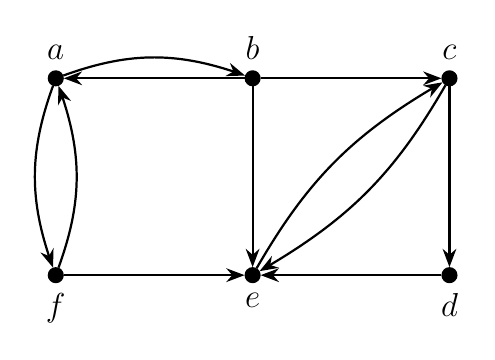
\begin{tikzpicture}[
    >=Stealth, % Modern, clean arrowheads
    thick,
    node distance=2.5cm,
    vertex/.style={circle, draw, fill=black, inner sep=0pt, minimum size=5pt},
    font=\large\itshape
]

    % ==========================================
    % VERTICES (Grid Layout)
    % ==========================================
    % Top Row
    \node[vertex, label=above:$a$] (a) at (0, 2.5) {};
    \node[vertex, label=above:$b$] (b) at (2.5, 2.5) {};
    \node[vertex, label=above:$c$] (c) at (5.0, 2.5) {};
    
    % Bottom Row
    \node[vertex, label=below:$f$] (f) at (0, 0) {};
    \node[vertex, label=below:$e$] (e) at (2.5, 0) {};
    \node[vertex, label=below:$d$] (d) at (5.0, 0) {};

    % ==========================================
    % DIRECTED EDGES
    % ==========================================
    
    % Between a and b
    \draw[->] (a) to[bend left=20] (b);
    \draw[->] (b) -- (a);
    
    % Between a and f
    \draw[->] (a) to[bend right=20] (f);
    \draw[->] (f) to[bend right=20] (a);
    
    % Between b and c
    \draw[->] (b) -- (c);
    
    % Between b and e
    \draw[->] (b) -- (e);
    
    % Between c and e (Two-way curved paths)
    \draw[->] (e) to[bend left=15] (c);
    \draw[->] (c) to[bend left=15] (e);
    
    % Between c and d
    \draw[->] (c) -- (d);
    
    % Between d and e
    \draw[->] (d) -- (e);
    
    % Between f and e
    \draw[->] (f) -- (e);

\end{tikzpicture}
\end{center}

\mk{6} \yr{CSE 103 | L-1/T-2 | 2015--16}

%% 2016-17
\item Define simple graph, multigraph, and digraph. Give examples of the following types of graphs: (i) simple directed graph, (ii) pseudograph, and (iii) directed pseudograph. Also show the adjacency matrices of your example graphs.
\mk{15} \yr{CSE 103 | L-1/T-2 | 2015--16}

%% 2015-16
\item What is a bipartite graph? Show that a simple graph is bipartite if and only if it is possible to assign one of two different colours to each vertex of the graph so that no two adjacent vertices are assigned the same colour.
\mk{7} \yr{CSE 103 | L-1/T-2 | 2015--16}

%% 2015-16
\item How many subgraphs with at least one vertex does $W_3$ (the wheel graph with four vertices) have?
\mk{7} \yr{CSE 103 | L-1/T-2 | 2015--16}

%% 2015-16
\item Show that in a simple graph with at least two vertices, there must be two vertices that have the same degree.
\mk{7} \yr{CSE 103 | L-1/T-2 | 2015--16}

%% 2016-17
\item Schedule the final exams for courses CSE1, CSE2, CSE3, CSE4 and ME101, ME201, ME301, ME401 using the fewest possible number of different time slots, given that there are no students taking both of the following pairs of courses: (ME101, CSE4), (ME201, CSE4), (ME401, CSE1), (ME401, CSE2), (ME101, ME201), (ME101, ME301), (ME301, ME401), but there are students enrolled in every other combination of courses. Use a graph colouring model to solve this problem.
\mk{15} \yr{CSE 103 | L-1/T-2 | 2013--14}

%% 2013-14
\item For the given traffic flow intersection, design a traffic signal pattern using graph colouring.

\begin{center}
  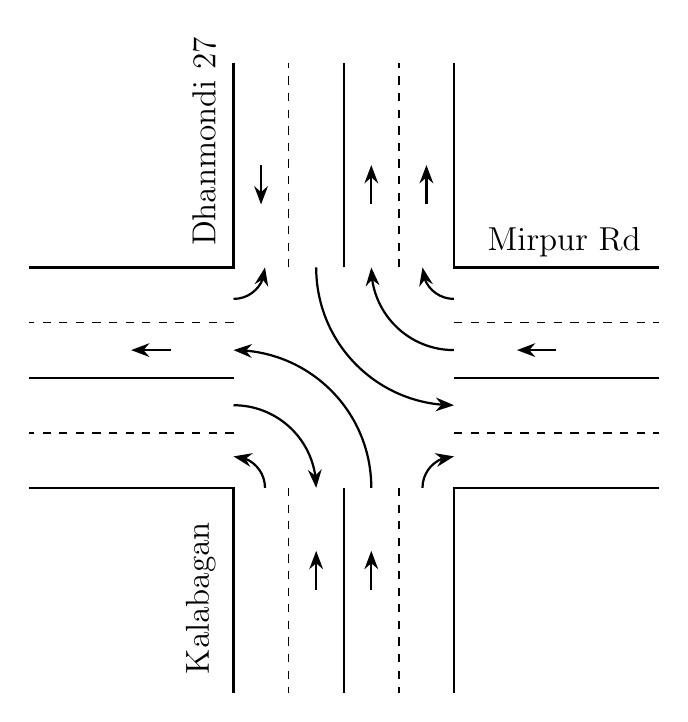
\begin{tikzpicture}[>=Stealth, line width=0.8pt]

    % --- Road Outlines (Curbs) ---
    % Top-Left Curb
    \draw[thick] (-1.4, 4.0) -- (-1.4, 1.4) -- (-4.0, 1.4);
    % Top-Right Curb
    \draw[thick] (1.4, 4.0) -- (1.4, 1.4) -- (4.0, 1.4);
    % Bottom-Left Curb
    \draw[thick] (-1.4, -4.0) -- (-1.4, -1.4) -- (-4.0, -1.4);
    % Bottom-Right Curb
    \draw[thick] (1.4, -4.0) -- (1.4, -1.4) -- (4.0, -1.4);

    % --- Center Solid Dividers ---
    \draw[thick] (0, 1.4) -- (0, 4.0);    % Top
    \draw[thick] (0, -1.4) -- (0, -4.0);  % Bottom
    \draw[thick] (-1.4, 0) -- (-4.0, 0);  % Left
    \draw[thick] (1.4, 0) -- (4.0, 0);    % Right

    % --- Lane Dividers (Dashed Lines) ---
    \draw[dashed, line width=0.6pt] (-0.7, 1.4) -- (-0.7, 4.0);  % Top-Left
    \draw[dashed, line width=0.6pt] (0.7, 1.4) -- (0.7, 4.0);    % Top-Right
    \draw[dashed, line width=0.6pt] (-0.7, -1.4) -- (-0.7, -4.0);% Bottom-Left
    \draw[dashed, line width=0.6pt] (0.7, -1.4) -- (0.7, -4.0);  % Bottom-Right
    
    \draw[dashed, line width=0.6pt] (-1.4, 0.7) -- (-4.0, 0.7);  % Left-Top
    \draw[dashed, line width=0.6pt] (-1.4, -0.7) -- (-4.0, -0.7);% Left-Bottom
    \draw[dashed, line width=0.6pt] (1.4, 0.7) -- (4.0, 0.7);    % Right-Top
    \draw[dashed, line width=0.6pt] (1.4, -0.7) -- (4.0, -0.7);  % Right-Bottom

    % --- Central Interlocking Loop Curves ---
    % Top-Incoming to Right-Outgoing
    \draw[->, thick] (-0.35, 1.4) to[out=-90, in=180] (1.4, -0.35);
    % Right-Incoming to Top-Outgoing
    \draw[->, thick] (1.4, 0.35) to[out=180, in=-90] (0.35, 1.4);
    % Bottom-Incoming to Left-Outgoing
    \draw[->, thick] (0.35, -1.4) to[out=90, in=0] (-1.4, 0.35);
    % Left-Incoming to Bottom-Outgoing
    \draw[->, thick] (-1.4, -0.35) to[out=0, in=90] (-0.35, -1.4);

    % --- Corner Filter/Turning Arrows ---
    % Top-Left Corner Turn
    \draw[->, thick] (-1.4, 1.0) to[out=0, in=-90] (-1.0, 1.4);
    % Bottom-Left Corner Turn
    \draw[->, thick] (-1.0, -1.4) to[out=90, in=0] (-1.4, -1.0);
    % Bottom-Right Corner Turn
    \draw[->, thick] (1.0, -1.4) to[out=90, in=180] (1.4, -1.0);
    % Top-Right Corner Turn
    \draw[->, thick] (1.4, 1.0) to[out=180, in=-90] (1.0, 1.4);

    % --- Straight/Lane Arrows ---
    % Top Road
    \draw[<-, thick] (-1.05, 2.2) -- (-1.05, 2.7);
    \draw[->, thick] (0.35, 2.2) -- (0.35, 2.7);
    \draw[->, thick] (1.05, 2.2) -- (1.05, 2.7);
    
    % Right Road
    \draw[->, thick] (2.7, 0.35) -- (2.2, 0.35);
    
    % Bottom Road
    \draw[<-, thick] (-0.35, -2.2) -- (-0.35, -2.7);
    \draw[->, thick] (0.35, -2.7) -- (0.35, -2.2);

    % Left Road
    \draw[->, thick] (-2.2, 0.35) -- (-2.7, 0.35);

    % --- Text Labels ---
    \node[rotate=90, anchor=south] at (-1.5, 3) {\large Dhanmondi 27};
    \node[rotate=90, anchor=south] at (-1.5, -2.8) {\large Kalabagan};
    \node[anchor=south] at (2.8, 1.4) {\large Mirpur Rd};

\end{tikzpicture}
\end{center}
\mk{15} \yr{CSE 103 | L-1/T-2 | 2013--14}


%% Jan 2021 — MRT scheduling
\item \begin{enumerate}
  \item Draw the cycle $C_8$. Then using $C_8$, draw the wheel $W_8$.
  \item Is there a simple graph whose degree sequence is 4, 3, 2, 1, 0? Justify your answer.
  \item Is the cycle $C_8$ bipartite or not? Explain with a figure.
\end{enumerate}
\mk{5+5+5} \yr{CSE 103 | L-1/T-2 | 2012--13}

%% 2013-14
\item At a party there are $n$ hosts and $m$ guests. Each guest shakes hands with each host, and each guest also shakes hands with each other guest. How can you find the total number of handshakes using a graph model?
\mk{6} \yr{CSE 103 | L-1/T-2 | 2011--12}

%% 2012-13
\item Seven towns $a, b, c, d, e, f$ and $g$ are connected by highways as follows:
\begin{itemize}[leftmargin=1.8em,itemsep=2pt,label={$\bullet$}]
  \item I-22 goes from $a$ to $c$, passing through $b$.
  \item I-33 goes from $c$ to $d$ and then passes through $b$ as it continues to $f$.
  \item I-44 goes from $d$ through $e$ to $a$.
  \item I-55 goes from $f$ to $b$, passing through $g$.
  \item I-66 goes from $g$ to $d$.
\end{itemize}
\begin{enumerate}
  \item Draw a graph model for the above road system.
  \item Find the adjacency matrix for the model.
  \item Is it possible to leave town $c$ and return there, visiting each of the other towns exactly once?
\end{enumerate}
\mk{4+4+4} \yr{CSE 103 | L-1/T-2 | 2010--11}

%% 2010-11
\item Find the chromatic number of the given tree.
\begin{center}
   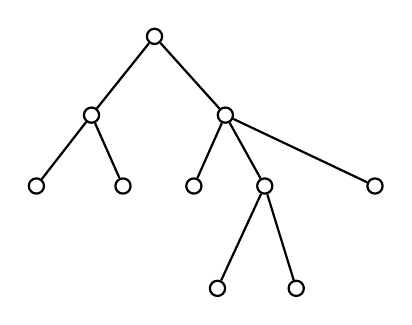
\begin{tikzpicture}[
        % ফাঁপা ও ছোট সার্কেল নোড স্টাইল (ছবির মতো)
        every node/.style={circle, draw=black, fill=white, inner sep=0pt, minimum size=5.5pt, thick},
        line width=0.8pt
    ]

    % --- ১. নোড বা ভার্টেক্সগুলোর পজিশন (Coordinates) ---
    
    % লেভেল ০ (শীর্ষ নোড)
    \node (root)  at (2.5, 4.2) {};

    % লেভেল ১
    \node (l1_l)  at (1.7, 3.2) {};
    \node (l1_r)  at (3.4, 3.2) {};

    % লেভেল ২
    \node (l2_1)  at (1.0, 2.3) {};
    \node (l2_2)  at (2.1, 2.3) {};
    \node (l2_3)  at (3.0, 2.3) {};
    \node (l2_4)  at (3.9, 2.3) {};
    \node (l2_5)  at (5.3, 2.3) {}; % ডানদিকের দীর্ঘ একক ব্রাঞ্চ

    % লেভেল ৩ (একদম নিচের চাইল্ড নোড দুটি)
    \node (l3_1)  at (3.3, 1.0) {};
    \node (l3_2)  at (4.3, 1.0) {};


    % --- ২. এজ বা কানেকশনগুলো ড্র করা (Tree Edges) ---
    \draw (root) -- (l1_l);
    \draw (root) -- (l1_r);

    \draw (l1_l) -- (l2_1);
    \draw (l1_l) -- (l2_2);

    \draw (l1_r) -- (l2_3);
    \draw (l1_r) -- (l2_4);
    \draw (l1_r) -- (l2_5); % ডানদিকের দীর্ঘ এজ

    \draw (l2_4) -- (l3_1);
    \draw (l2_4) -- (l3_2);



    \end{tikzpicture}
\end{center}

\mk{3} \yr{CSE 103 | L-1/T-2 | 2010--11}


%% 2015-16
\item Prove that an undirected graph has an even number of vertices with odd degree.
\mk{5} \yr{CSE 103 | L-1/T-2 | 2009--10}

%% 2010-11
\item Prove that in any graph, the number of nodes of odd degree is even.
\mk{10} \yr{CSE 103 | L-1/T-2 | 2008--09}

%% 2008-09
\item Either find a graph that models the following situation or show that none exists: Each of the 50 students will be assigned the use of 1 of 25 computers, and each of the 25 computers will be used by exactly 1 or 3 students.
\mk{10} \yr{CSE 103 | L-1/T-2 | 2008--09}

%% 2008-09
\item Find the edge connectivity of the following graph.
\begin{center}
      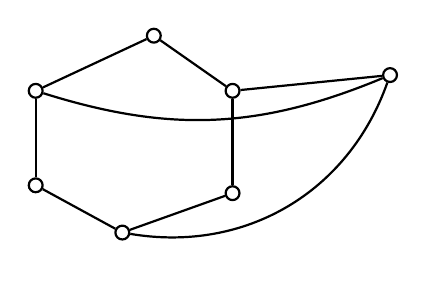
\begin{tikzpicture}[
        every node/.style={circle, draw=black, fill=white, inner sep=0pt, minimum size=5pt, thick},
        line width=0.8pt
    ]
        % --- নোড বা ভার্টেক্সগুলোর পজিশন ডিফাইন (Coordinates) ---
        
        % ওপরের ৩টি নোড (Roof/Top structure)
        \node (t_left)  at (0,2) {};
        \node (t_mid)   at (1.5,2.7) {};
        \node (t_right) at (2.5,2) {};
        
        % নিচের ৪টি নোড (Base structure)
        \node (b_left)  at (0,0.8) {};
        \node (b_bot)   at (1.1,0.2) {};
        \node (b_right) at (2.5,0.7) {};
        
        % ডানপাশের এক্সট্রা নোড (Far right extended vertex)
        \node (ext)     at (4.5,2.2) {};

        % --- এজ বা কানেকশনগুলো ড্র করা (Edges) ---
        
        % ওপরে ঘরের চালের মতো অংশ
        \draw (t_left) -- (t_mid);
        \draw (t_mid) -- (t_right);
        
        % ভার্টিকাল বা খাড়া এজগুলো
        \draw (t_left) -- (b_left);
        \draw (t_right) -- (b_right);
        
        % নিচের লুপ/বেস অংশ
        \draw (b_left) -- (b_bot);
        \draw (b_bot) -- (b_right);
        
        % ডানপাশের এক্সট্রা নোডের সাথে কানেকশন
        \draw (t_right) -- (ext);
        
        % কার্ভড লাইন বা বাঁকানো এজগুলো (Curved Edges)
        \draw (t_left) to[bend right=20] (ext);   % বামের ওপর থেকে ডানের শেষ নোড পর্যন্ত বাঁকানো লাইন
        \draw (b_bot) to[bend right=40] (ext);    % একদম নিচের নোড থেকে ডানের শেষ নোড পর্যন্ত নিচ দিয়ে বাঁকানো লাইন

    \end{tikzpicture}
\end{center}

\mk{6} \yr{CSE 103 | L-1/T-2 | 2008--09}


%% 2022-23
\end{enumerate}

%%──────────────────────────────────────────────────────────────────────
\subtopic{cE}{Planar Graphs}
\label{sub:s9-planargraphs}

\begin{enumerate}


  %% 2008-09
\item A disaster area map is represented by $N$ villages which form a planar graph. The 8 vertices of that graph have degrees 4, 3, 4, 3, 3, 3, 3, 3. How many villages can be mapped in that area? Justify your finding.
\mk{10} \yr{CSE 103 | L-1/T-1 | 2023--24}

\item For a loop-free connected planar graph $G(V, E)$ with $|V| = v$ and $|E| = e > 2$ and $r$ regions, prove that $3r \leq 2e$ and $e \leq 3v - 6$.
\mk{7} \yr{CSE 103 | L-1/T-2 | 2013--14}

%% 2023-24
\item Prove Euler's Formula: Let $G$ be a connected planar simple graph with $e$ edges and $v$ vertices. Let $r$ be the number of regions in a planar representation of $G$. Then $r = e - v + 2$.
\mk{7/15/17/10} \yr{CSE 103 | L-1/T-2 | 2016--17, 2013--14, 2012--13, 2011--12, 2009--10}


%% 2011-12
\item Find a planar representation of the given graph or show that none exists.
\begin{center}
      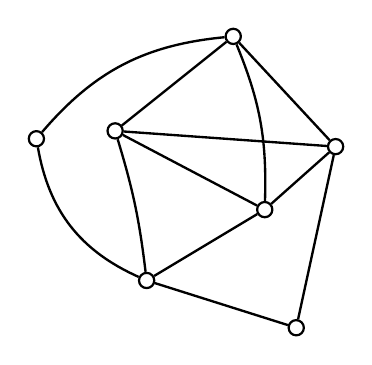
\begin{tikzpicture}[
        every node/.style={circle, draw=black, fill=white, inner sep=0pt, minimum size=5.5pt, thick},
        line width=0.85pt % ছবির স্কেচ লাইনের মতো স্ট্রং থিকনেস
    ]
        % --- নোড বা ভার্টেক্সগুলোর পজিশন (Coordinates) ---
        
        \node (top)    at (2,4) {};       % শীর্ষের নোড
        \node (left)   at (0.5,2.8) {};   % ভেতরের বামের নোড
        \node (right)  at (3.3,2.6) {};   % ডানের নোড
        \node (center) at (2.4,1.8) {};   % মাঝখানের নোড
        \node (bot_l)  at (0.9,0.9) {};   % নিচের বামের নোড
        \node (bot_r)  at (2.8,0.3) {};   % নিচের ডানের নোড
        \node (ext_l)  at (-0.5,2.7) {};  % একদম বাইরের বামের একক নোড

        % --- এজ বা কানেকশনগুলো ড্র করা (Edges) ---
        
        % সোজা প্রধান এজগুলো (Straight edges)
        \draw (top) -- (left);
        \draw (top) -- (right);
        \draw (left) -- (right);
        \draw (left) -- (center);
        \draw (center) -- (bot_l);
        \draw (center) -- (right);
        \draw (right) -- (bot_r);
        \draw (bot_l) -- (bot_r);
        
        % ছবির সাথে মিলিয়ে কার্ভড বা বাঁকানো এজগুলো (Curved Edges strictly based on image)
        
        % ১. বামের ভেতরের নোড থেকে নিচের নোডে হালকা ইনওয়ার্ড কার্ভ
        \draw (left) to[bend left=5] (bot_l); 
        
        % ২. শীর্ষের নোড (top) থেকে মাঝখানের নোডে (center) কার্ভটি ডানদিকে বাঁকানো
        \draw (top) to[bend left=12] (center);
        
        % ৩. একদম বাইরের বামের নোড (ext_l) থেকে ওপরের নোডে কার্ভ
        \draw (ext_l) to[bend left=22] (top);
        
        % ৪. একদম বাইরের বামের নোড (ext_l) থেকে নিচের বামের নোডে (bot_l) কার্ভ
        \draw (ext_l) to[bend right=28] (bot_l);

    \end{tikzpicture}
\end{center}

\mk{6} \yr{CSE 103 | L-1/T-2 | 2008--09}

%% 2009-10
\end{enumerate}

%%──────────────────────────────────────────────────────────────────────
\subtopic{cE}{Graph Isomorphism}
\label{sub:s9-isomorphism}

\begin{enumerate}


%% 2011-12
\item Determine if the path planning graphs $P$ and $P'$ of two book-collecting robots are isomorphic or not. The robots stop and collect books at some shelves for a while; these shelves are represented by vertices. Give the reasoning of your answer.

\begin{center}
  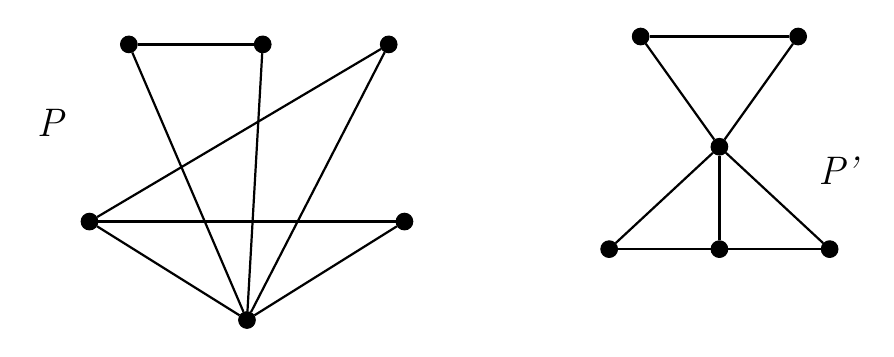
\begin{tikzpicture}[
    % Style for the vertices/nodes
    vertex/.style={circle, draw, fill=black, inner sep=0pt, minimum size=6pt},
    % Style for the edges/lines
    edge/.style={thick, black},
    % Style for labels
    label style/.style={font=\Large\itshape}
]

    % ==========================================
    % GRAPH P (Left Side)
    % ==========================================
    
    % Coordinates for Graph P
    \node[vertex] (P_bottom) at (2,-2) {};
    \node[vertex] (P_mid_left) at (0,-0.75) {};
    \node[vertex] (P_mid_right) at (4,-0.75) {};
    
    \node[vertex] (P_top_left) at (0.5,1.5) {};
    \node[vertex] (P_top_mid) at (2.2,1.5) {};
    \node[vertex] (P_top_right) at (3.8,1.5) {};
    
    % Label for Graph P
    \node[label style] at (-0.5,0.5) {P};

    % Edges for Graph P
    \draw[edge] (P_mid_left) -- (P_mid_right);
    \draw[edge] (P_top_left) -- (P_top_mid);
    
    \draw[edge] (P_bottom) -- (P_mid_left);
    \draw[edge] (P_bottom) -- (P_mid_right);
    \draw[edge] (P_bottom) -- (P_top_left);
    \draw[edge] (P_bottom) -- (P_top_mid);
    \draw[edge] (P_bottom) -- (P_top_right);
    
    \draw[edge] (P_mid_left) -- (P_top_right);

    % ==========================================
    % GRAPH P' (Right Side)
    % ==========================================
    
    % Coordinates for Graph P' (shifted to the right by 7 units)
    \node[vertex] (Pp_center) at (8,0.2) {};
    
    \node[vertex] (Pp_top_left) at (7.0,1.6) {};
    \node[vertex] (Pp_top_right) at (9.0,1.6) {};
    
    \node[vertex] (Pp_bot_left) at (6.6,-1.1) {};
    \node[vertex] (Pp_bot_mid) at (8.0,-1.1) {};
    \node[vertex] (Pp_bot_right) at (9.4,-1.1) {};
    
    % Label for Graph P'
    \node[label style] at (9.5, -0.1) {P'};

    % Edges for Graph P'
    % Top triangle structure
    \draw[edge] (Pp_top_left) -- (Pp_top_right);
    \draw[edge] (Pp_center) -- (Pp_top_left);
    \draw[edge] (Pp_center) -- (Pp_top_right);
    
    % Bottom fan structure
    \draw[edge] (Pp_bot_left) -- (Pp_bot_mid) -- (Pp_bot_right);
    \draw[edge] (Pp_center) -- (Pp_bot_left);
    \draw[edge] (Pp_center) -- (Pp_bot_mid);
    \draw[edge] (Pp_center) -- (Pp_bot_right);

\end{tikzpicture}
\end{center}

\mk{8} \yr{CSE 103 | L-1/T-1 | 2023--24}



\item Consider the two bus routes represented by graphs $G$ and $G'$ as shown below. Bus stops are represented by vertices in $G$ and $G'$. Consider the mapping $g: V(G) \rightarrow V(G')$ between the vertices in G and G' (as shown below). Does this mapping represent an isomorphism between $G$ and $G'$?
\begin{center}
      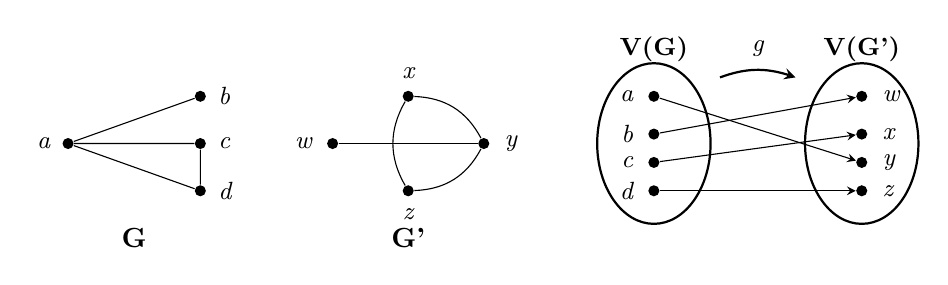
\begin{tikzpicture}[
        scale=1.2,
        dot/.style={circle, fill=black, inner sep=0pt, minimum size=4pt},
        font=\itshape\small
    ]

        % ==================== GRAPH G ====================
        \begin{scope}[shift={(0,0)}]
            \node[dot] (ga) at (0, 0.7) {};
            \node[left=3pt] at (ga) {a};
            
            \node[dot] (gb) at (1.4, 1.2) {};
            \node[right=3pt] at (gb) {b};
            
            \node[dot] (gc) at (1.4, 0.7) {};
            \node[right=3pt] at (gc) {c};
            
            \node[dot] (gd) at (1.4, 0.2) {};
            \node[right=3pt] at (gd) {d};

            \draw (ga) -- (gb);
            \draw (ga) -- (gc);
            \draw (ga) -- (gd);
            \draw (gc) -- (gd);
            
            \node[draw=none, font=\bfseries\upshape] at (0.7, -0.3) {G};
        \end{scope}

        % ==================== GRAPH G' ====================
        \begin{scope}[shift={(2.8,0)}]
            \node[dot] (gw) at (0, 0.7) {};
            \node[left=4pt] at (gw) {w};
            
            \node[dot] (gx) at (0.8, 1.2) {};
            \node[above=3pt] at (gx) {x};
            
            \node[dot] (gz) at (0.8, 0.2) {};
            \node[below=3pt] at (gz) {z};

            \node[dot] (gy) at (1.6, 0.7) {};
            \node[right=4pt] at (gy) {y};

            \draw (gw) -- (gy);
            
            \draw (gz) to[bend left=30] (gx);
            \draw (gx) to[bend left=30] (gy);
            
            \draw (gz) to[bend right=30] (gy);
            
            \node[draw=none, font=\bfseries\upshape] at (0.8, -0.3) {G'};
        \end{scope}

        % ==================== MAPPING ====================
        \begin{scope}[shift={(6.2,0)}]
            % ওভাল/ডিম্বাকৃতি সেট (Ellipses for Sets)
            \draw[thick] (0, 0.7) ellipse (0.6cm and 0.85cm);
            \draw[thick] (2.2, 0.7) ellipse (0.6cm and 0.85cm);
            
            \node[above=26pt, font=\bfseries\upshape\small] at (0, 0.7) {V(G)};
            \node[above=26pt, font=\bfseries\upshape\small] at (2.2, 0.7) {V(G')};
            
            \node[dot] (ma) at (0, 1.2) {}; \node[left=4pt] at (ma) {a};
            \node[dot] (mb) at (0, 0.8) {}; \node[left=4pt] at (mb) {b};
            \node[dot] (mc) at (0, 0.5) {}; \node[left=4pt] at (mc) {c};
            \node[dot] (md) at (0, 0.2) {}; \node[left=4pt] at (md) {d};

            \node[dot] (mw) at (2.2, 1.2) {}; \node[right=4pt] at (mw) {w};
            \node[dot] (mx) at (2.2, 0.8) {}; \node[right=4pt] at (mx) {x};
            \node[dot] (my) at (2.2, 0.5) {}; \node[right=4pt] at (my) {y};
            \node[dot] (mz) at (2.2, 0.2) {}; \node[right=4pt] at (mz) {z};

            \draw[->, >=stealth] (ma) -- (my);
            \draw[->, >=stealth] (mb) -- (mw);
            \draw[->, >=stealth] (mc) -- (mx);
            \draw[->, >=stealth] (md) -- (mz);
            
            \draw[->, >=stealth, thick] (0.7, 1.4) to[bend left=20] node[above=1pt] {g} (1.5, 1.4);
        \end{scope}

    \end{tikzpicture}
\end{center}

\mk{10} \yr{CSE 103 | L-1/T-I | 2021--22}

%% 2010-11
\item A function $f$ is defined as: $f(A)=q,\, f(B)=v,\, f(C)=u,\, f(D)=y,\, f(E)=r,\, f(F)=w,\, f(G)=x,\, f(H)=t,\, f(I)=z,\, f(J)=s$. If a graph $M$ is mapped to graph $N$ after applying function $f$, determine whether $M$ and $N$ are isomorphic or not.
\begin{center}
      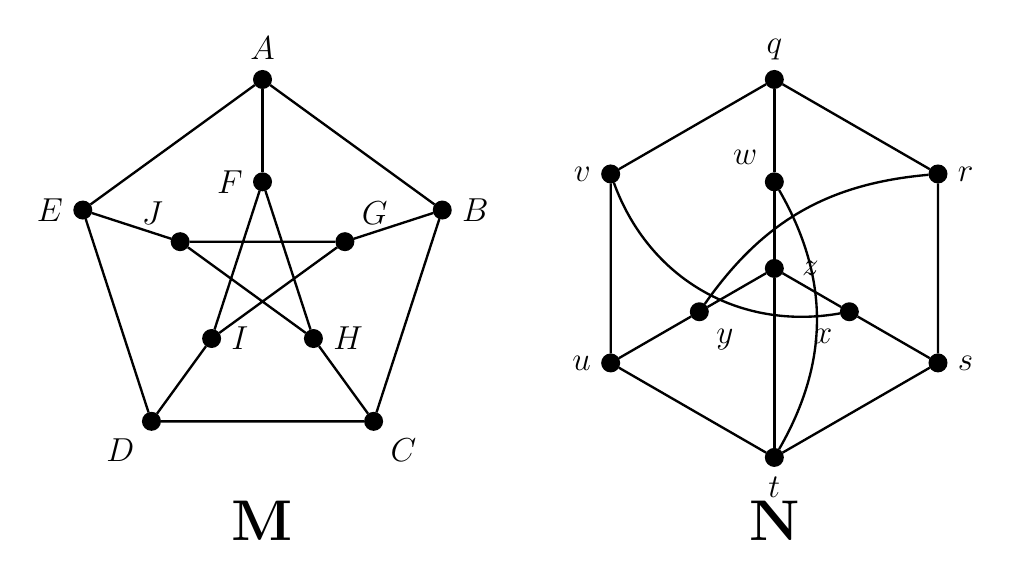
\begin{tikzpicture}[
        % নোড এবং টেক্সটের স্ট্যান্ডার্ড সাইজ ও থিকনেস স্টাইল
        vertex/.style={circle, draw=black, fill=black, inner sep=0pt, minimum size=6pt},
        line width=0.85pt,
        % লেবেলের ফন্ট সাইজ এবং স্টাইল এখানে ডিফাইন করে এরর ফিক্স করা হলো
        label style/.style={font=\large}
    ]

    % =================================================================
    %                      LEFT GRAPH (u-nodes: Graph M)
    % =================================================================
    \begin{scope}[shift={(0,0)}]
        % বাইরের পেন্টাগনের নোডসমূহ (Outer Pentagon - 72 deg spacing)
        \node[vertex, label={[label style]left:$E$}] (u1) at (162:2.4) {};
        \node[vertex, label={[label style]above:$A$}] (u2) at (90:2.4) {};
        \node[vertex, label={[label style]right:$B$}] (u3) at (18:2.4) {};
        \node[vertex, label={[label style]below right:$C$}] (u4) at (306:2.4) {};
        \node[vertex, label={[label style]below left:$D$}] (u5) at (234:2.4) {};

        % ভেতরের স্টারের নোডসমূহ (Inner Star)
        \node[vertex, label={[label style]above left:$J$}] (u10) at (162:1.1) {};
        \node[vertex, label={[label style]left:$F$}] (u9) at (90:1.1) {};
        \node[vertex, label={[label style]above right:$G$}] (u8) at (18:1.1) {};
        \node[vertex, label={[label style]right:$H$}] (u7) at (306:1.1) {};
        \node[vertex, label={[label style]right:$I$}] (u6) at (234:1.1) {};

        % বাইরের পেন্টাগনের এজসমূহ (Outer Ring)
        \draw (u1) -- (u2) -- (u3) -- (u4) -- (u5) -- (u1);

        % বাইর থেকে ভেতরের কানেক্টিং এজসমূহ (Spokes)
        \draw (u1) -- (u10);
        \draw (u2) -- (u9);
        \draw (u3) -- (u8);
        \draw (u4) -- (u7);
        \draw (u5) -- (u6);

        % ভেতরের স্টারের এজসমূহ (Inner Star Connections)
        \draw (u10) -- (u8) -- (u6) -- (u9) -- (u7) -- (u10);
        
        % গ্রাফের নিচে M লেবেল যোগ করা হলো
        \node[draw=none, fill=none, font=\huge\bfseries] at (270:3.2) {M};
    \end{scope}


    % =================================================================
    %                      RIGHT GRAPH (v-nodes: Graph N)
    % =================================================================
    \begin{scope}[shift={(6.5,0)}] % ডানপাশে পর্যাপ্ত দূরত্বে শিফট করা হলো
        % বাইরের হেক্সাগন নোডসমূহ (Outer Hexagon Structure)
        \node[vertex, label={[label style]left:$v$}] (v1) at (150:2.4) {};
        \node[vertex, label={[label style]above:$q$}] (v2) at (90:2.4) {};
        \node[vertex, label={[label style]right:$r$}] (v3) at (30:2.4) {};
        \node[vertex, label={[label style]right:$s$}] (v4) at (330:2.4) {};
        \node[vertex, label={[label style]below:$t$}] (v5) at (270:2.4) {};
        \node[vertex, label={[label style]left:$u$}] (v6) at (210:2.4) {};

        % ভেতরের নোডসমূহ (Inner Matrix-like Layout)
        \node[vertex, label={[label style]above left:$w$}] (v8) at (90:1.1) {};
        \node[vertex, label={[label style]below right:$y$}] (v7) at (210:1.1) {};
        \node[vertex, label={[label style]below left:$x$}] (v9) at (330:1.1) {};
        \node[vertex, label={[label style]right:\hspace{0.1cm}$z$}] (v10) at (0,0) {}; % সেন্ট্রাল নোড

        % বাইরের হেক্সাগনের এজসমূহ
        \draw (v1) -- (v2) -- (v3) -- (v4) -- (v5) -- (v6) -- (v1);

        % ভেতরের সেন্ট্রাল ও帮স্পোক কানেকশনস (Straight Lines)
        \draw (v2) -- (v8);
        \draw (v5) -- (v10);
        \draw (v6) -- (v7);
        \draw (v4) -- (v9);
        \draw (v8) -- (v10);
        \draw (v7) -- (v10);
        \draw (v9) -- (v10);

        % ছবির কাস্টম কার্ভড এজসমূহ (Curved Edges strictly based on image)
        \draw (v1) to[bend right=40] (v9);
        \draw (v3) to[bend right=25] (v7);
        \draw (v5) to[bend right=30] (v8);

        % গ্রাফের নিচে N লেবেল যোগ করা হলো
        \node[draw=none, fill=none, font=\huge\bfseries] at (270:3.2) {N};
    \end{scope}

    \end{tikzpicture}
\end{center}

\mk{5/3} \yr{CSE 103 | L-1/T-2 | 2013--14, 2010--11}



%% 2023-24
\item Let $f$ be a one-to-one correspondence between the vertex set of graph $G$ and the vertex set of graph $H$, defined as: $f(u_1)=v_1$, $f(u_2)=v_2$, $f(u_3)=v_4$, $f(u_4)=v_3$, $f(u_5)=v_5$, $f(u_6)=v_7$, $f(u_7)=v_6$, $f(u_8)=v_8$. Show whether $f$ is an isomorphism or not.
\begin{center}
        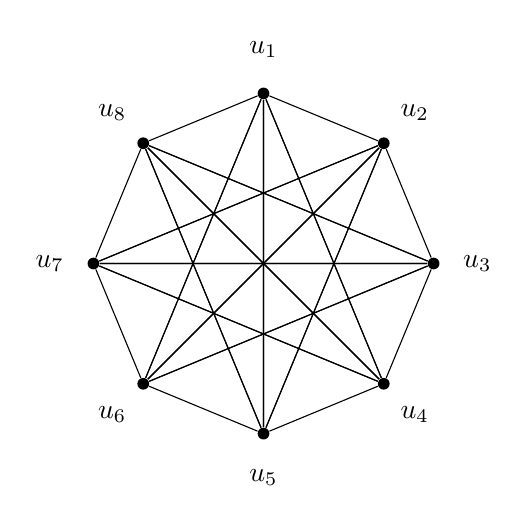
\begin{tikzpicture}[scale=1.8, every node/.style={circle, fill=black, inner sep=1.5pt}]
            % Place vertices u_1 to u_8 in a circle (starting from top, moving clockwise)
            \foreach \i/\label [count=\n] in {1/1, 2/2, 3/3, 4/4, 5/5, 6/6, 7/7, 8/8} {
                % 90 - (\n-1)*45 degrees places vertex 1 at the top (90 deg)
                \node (u\i) at ({90 - (\n-1)*45}:1.2) {};
                % Label positioning
                \node[fill=none, draw=none, anchor={90 - (\n-1)*45 + 180}] at ({90 - (\n-1)*45}:1.35) {$u_{\label}$};
            }
            
            % Draw the outer octagon perimeter
            \draw (u1) -- (u2) -- (u3) -- (u4) -- (u5) -- (u6) -- (u7) -- (u8) -- cycle;
            
            % Draw internal chords for Graph G
            \draw (u1) -- (u4) (u1) -- (u5) (u1) -- (u6);
            \draw (u2) -- (u5) (u2) -- (u6) (u2) -- (u7);
            \draw (u3) -- (u6) (u3) -- (u7) (u3) -- (u8);
            \draw (u4) -- (u7) (u4) -- (u8) (u4) -- (u1);
            \draw (u5) -- (u8) (u5) -- (u1) (u5) -- (u2);
            \draw (u6) -- (u1) (u6) -- (u2) (u6) -- (u3);
            \draw (u7) -- (u2) (u7) -- (u3) (u7) -- (u4);
            \draw (u8) -- (u3) (u8) -- (u4) (u8) -- (u5);
            \draw (u8) -- (u1) ;
        \end{tikzpicture}
        \textbf{$G$}

        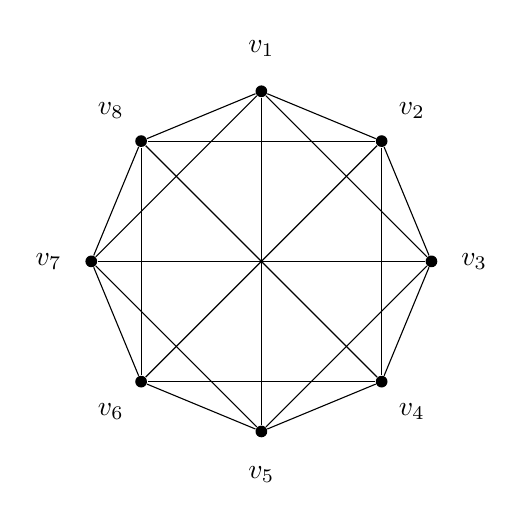
\begin{tikzpicture}[scale=1.8, every node/.style={circle, fill=black, inner sep=1.5pt}]
            % Place vertices v_1 to v_8 in a circle
            \foreach \i/\label [count=\n] in {1/1, 2/2, 3/3, 4/4, 5/5, 6/6, 7/7, 8/8} {
                \node (v\i) at ({90 - (\n-1)*45}:1.2) {};
                \node[fill=none, draw=none, anchor={90 - (\n-1)*45 + 180}] at ({90 - (\n-1)*45}:1.35) {$v_{\label}$};
            }
            
            % Draw the outer octagon perimeter
            \draw (v1) -- (v2) -- (v3) -- (v4) -- (v5) -- (v6) -- (v7) -- (v8) -- cycle;
            
            % Draw internal chords for Graph H
            % Diagonal/Opposite lines
            \draw (v1) -- (v5);
            \draw (v2) -- (v6);
            \draw (v3) -- (v7);
            \draw (v4) -- (v8);
            \draw (v8) -- (v1);
            
            % Outer box skips (chords skipping 1 vertex)
            \draw (v1) -- (v3) (v3) -- (v5) (v5) -- (v7) (v7) -- (v1);
            \draw (v2) -- (v4) (v4) -- (v6) (v6) -- (v8) (v8) -- (v2);
          \end{tikzpicture}
          \textbf{$H$}
      
\end{center}      

\mk{6} \yr{CSE 103 | L-1/T-2 | 2011--12}

%% 2013-14
\end{enumerate}

%%──────────────────────────────────────────────────────────────────────
\subtopic{cE}{Paths, Euler \& Hamiltonian}
\label{sub:s9-paths}

\begin{enumerate}

%% 2015-16
\item A disaster area map with 8 vertices has degrees 4, 3, 4, 3, 3, 3, 3, 3. Find the minimum travel time if all connecting paths between villages require 3 hours of travel time, such that you visit each village only once.
\mk{5} \yr{CSE 103 | L-1/T-1 | 2023--24}

%% 2023-24
\item Chain stores $C_1, C_2, C_3, C_4, C_5, C_6, C_7$ are represented such that they have goods transaction channels with each other. Determine if a salesperson starting from $C_7$ can visit each path exactly once, cover all seven stores, and come back to $C_7$. Show all steps to find the path.
\mk{12} \yr{CSE 103 | L-1/T-1 | 2023--24}

%% 2022-23
\item There is a road network among cities $a, b, c, d, e, f, g, h, i, j$. Starting from $j$, determine how you can visit all places such that you travel each road \textbf{exactly once} and ultimately come back to $j$. Show all steps.
\begin{center}
      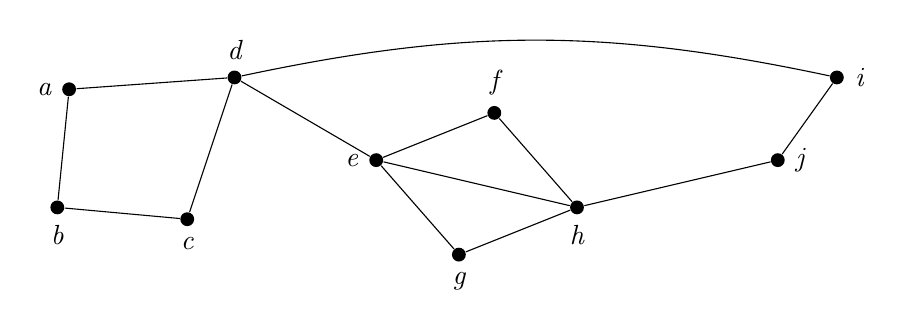
\begin{tikzpicture}[
        scale=1.5,
        % ছোট বৃত্তাকার নোড পয়েন্টার
        dot/.style={circle, fill=black, inner sep=0pt, minimum size=5pt},
        every node/.style={font=\itshape}
    ]

        % --- Nodes Positioning ---
        \node[dot] (a) at (0, 1.2) {};
        \node[left=3pt] at (a) {a};
        
        \node[dot] (b) at (-0.1, 0.2) {};
        \node[below=3pt] at (b) {b};
        
        \node[dot] (c) at (1.0, 0.1) {};
        \node[below=3pt] at (c) {c};
        
        \node[dot] (d) at (1.4, 1.3) {};
        \node[above=3pt] at (d) {d};
        
        \node[dot] (e) at (2.6, 0.6) {};
        \node[left=3pt] at (e) {e};
        
        \node[dot] (f) at (3.6, 1.0) {};
        \node[above=3pt] at (f) {f};
        
        \node[dot] (g) at (3.3, -0.2) {};
        \node[below=3pt] at (g) {g};
        
        \node[dot] (h) at (4.3, 0.2) {};
        \node[below=3pt] at (h) {h};
        
        \node[dot] (j) at (6.0, 0.6) {};
        \node[right=3pt] at (j) {j};
        
        \node[dot] (i) at (6.5, 1.3) {};
        \node[right=3pt] at (i) {i};


        % --- Edges (Connections) ---
        \draw (a) -- (b);
        \draw (b) -- (c);
        \draw (c) -- (d);
        \draw (d) -- (a);
        
        \draw (d) -- (e);
        \draw (e) -- (f);
        \draw (f) -- (h);
        \draw (e) -- (g);
        \draw (g) -- (h);
        \draw (e) -- (h); 
        
        \draw (h) -- (j);
        \draw (j) -- (i);
        
        % d থেকে i পর্যন্ত টপ কার্ভড লাইন
        \draw (d) to[bend left=12] (i);

    \end{tikzpicture}
\end{center}

\mk{13} \yr{CSE 103 | L-1/T-1 | 2022--23}

%% Session: 2021-2022
\item Five class friends exchange books among themselves. The exchanges can be represented by the given diagram. Each of them gives the book to one of the friends for only one time and cannot take back directly from that friend. For example, Jasim gives the book to Rani, Rani will read the book and she needs to pass the book to Rahim, or Malek, or Mina. Jasim cannot take the book back from Rani directly. Find if they can cover all exchanges if Jasim starts giving his CSE 103 text book to any of his friends. If the tour forms the Euler circuit, give the reason why it is an Euler circuit. (Show the steps of the tour.)
\begin{center}
  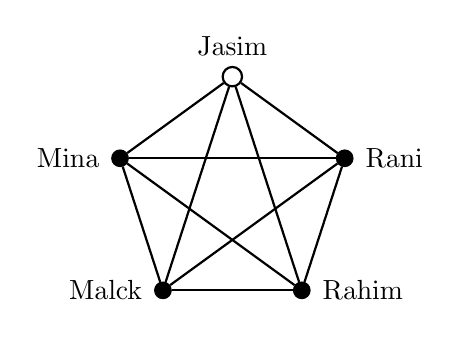
\begin{tikzpicture}[
        scale=1.5,
        % সাধারণ কালো নোড (ভেতরে কালো রঙ, লেখা বাইরে থাকবে)
        blackdot/.style={circle, fill=black, draw=black, inner sep=0pt, minimum size=6pt},
        % জসিম নোডের জন্য স্পেশাল সাদা নোড
        whitedot/.style={circle, fill=white, draw=black, thick, inner sep=0pt, minimum size=7pt}
    ]

    % --- Nodes Positioning (Using Angular Coordinates for Perfect Pentagon) ---
    % টপ নোড (Jasim) - ৯০ ডিগ্রিতে
    \node[whitedot] (Jasim) at (90:1.0) {};
    \node[above=4pt] at (Jasim) {Jasim};

    % বামের নোড (Mina) - ১৬২ ডিগ্রিতে
    \node[blackdot] (Mina) at (162:1.0) {};
    \node[left=4pt] at (Mina) {Mina};

    % ডানের নোড (Rani) - ১৮ ডিগ্রিতে
    \node[blackdot] (Rani) at (18:1.0) {};
    \node[right=4pt] at (Rani) {Rani};

    % নিচের বামের নোড (Malck) - ২৩৪ ডিগ্রিতে
    \node[blackdot] (Malck) at (234:1.0) {};
    \node[left=4pt] at (Malck) {Malck};

    % নিচের ডানের নোড (Rahim) - ৩০৬ ডিগ্রিতে
    \node[blackdot] (Rahim) at (306:1.0) {};
    \node[right=4pt] at (Rahim) {Rahim};


    % --- Edges (Complete Graph K_5 Connections) ---
    % বাইরের পঞ্চভুজের লাইনসমূহ
    \draw[thick] (Jasim) -- (Rani);
    \draw[thick] (Rani) -- (Rahim);
    \draw[thick] (Rahim) -- (Malck);
    \draw[thick] (Malck) -- (Mina);
    \draw[thick] (Mina) -- (Jasim);

    % ভেতরের স্টার বা ক্রস কানেকশনসমূহ
    \draw[thick] (Jasim) -- (Rahim);
    \draw[thick] (Jasim) -- (Malck);
    \draw[thick] (Mina) -- (Rani);
    \draw[thick] (Mina) -- (Rahim);
    \draw[thick] (Rani) -- (Malck);

    \end{tikzpicture}
\end{center}


\mk{13} \yr{CSE 103 | L-1/T-I | 2021--22}

\item Derive a proof of the following theorem: ``A connected graph has an Eulerian cycle if and only if every vertex is of even degree.''
\mk{15} \yr{CSE 103 | L-1/T-2 | 2020--21}  

%% Jan 2021
\item Is there any Euler cycle in the complete graph $K_5$? If it exists, write down the cycle.
\mk{3} \yr{CSE 103 | L-1/T-2 | Jan 2021}

%% 2009-10
\item A bus route is shown in a given graph. Find the adjacency list for the graph.\mk{8}
\begin{center}
  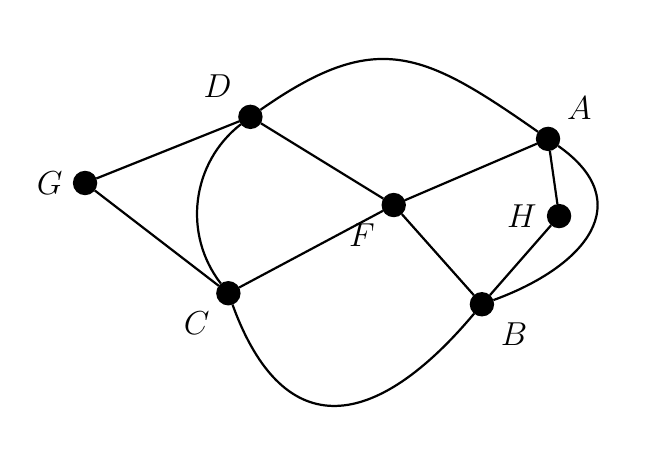
\begin{tikzpicture}[
    scale=1.4,
    thick,
    vertex/.style={circle, draw, fill=black, inner sep=0pt, minimum size=8pt},
    font=\sffamily\large
]

    % ==========================================
    % VERTICES (Positions configured to match image layout)
    % ==========================================
    \node[vertex, label=left:{$G$}] (G) at (0, 0.7) {};
    \node[vertex, label=above left:{$D$}] (D) at (1.5, 1.3) {};
    \node[vertex, label=below left:{$C$}] (C) at (1.3, -0.3) {};
    \node[vertex, label=below left:{$F$}] (F) at (2.8, 0.5) {};
    \node[vertex, label=below right:{$B$}] (B) at (3.6, -0.4) {};
    \node[vertex, label=left:{$H$}] (H) at (4.3, 0.4) {};
    \node[vertex, label=above right:{$A$}] (A) at (4.2, 1.1) {};

    % ==========================================
    % EDGES (Straight and Custom Curved)
    % ==========================================
    
    % Core connections around G, D, and C
    \draw (G) -- (D);
    \draw (G) -- (C);
    \draw (D) -- (F);
    \draw (C) -- (F);
    
    % Inner curved edge between D and C
    \draw (D) to[bend right=45] (C);
    
    % Core connections around Center (F) and Right Block
    \draw (F) -- (A);
    \draw (F) -- (B);
    \draw (A) -- (H);
    \draw (B) -- (H);
    
    % Long top-spanning curved edge from D to A
    \draw (D) to[out=35, in=145, looseness=1.3] (A);
    
    % Bottom-spanning curved edge from C to B
    \draw (C) to[out=-70, in=-130, looseness=1.6] (B);
    
    % Outer loop extension edge from A around to B
    \draw (A) to[out=-35, in=20, looseness=1.5] (B);

\end{tikzpicture}
\end{center}
Show that the bus route graph has an Euler circuit. Find the Euler circuit starting from node $F$. Show all steps.
\mk{10} \yr{CSE 103 | L-1/T-2 | Jan 2020}


%% 2009-10
\item Prove that for all $n \geq 3$, the number of distinct Hamiltonian cycles in $K_n$ is $\dfrac{(n-1)!}{2}$.
\mk{10} \yr{CSE 103 | L-1/T-2 | 2017--18}  

%% Jan 2020
\item What are Euler paths and Hamilton paths? Show that a connected multigraph with at least two vertices has an Euler circuit if and only if all of its vertices have even degree.
\mk{15} \yr{CSE 103 | L-1/T-2 | 2016--17}

%% 2017-18
\item Show that if a connected multigraph has an Euler path (but not an Euler circuit), then it has exactly two vertices of odd degree.
\mk{6} \yr{CSE 103 | L-1/T-2 | 2015--16}

%% 2016-17
\item Find the Euler circuit from the given graph starting from vertex $a$. Show all steps.
\begin{center}
      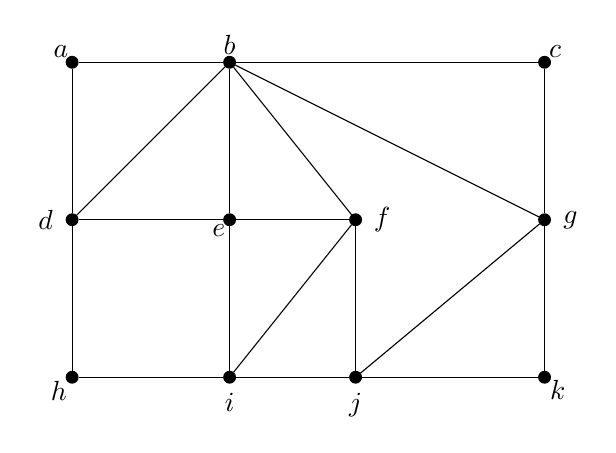
\begin{tikzpicture}[scale=2, every node/.style={circle, draw=black, fill=black, inner sep=1.5pt, minimum size=4pt}]
        
        % --- Define and Place Vertices (Grid Coordinates) ---
        % Top Row
        \node (a) at (0,2) {};
        \node (b) at (1,2) {};
        \node (c) at (3,2) {}; % Spaced further right out to match width
        
        % Middle Row
        \node (d) at (0,1) {};
        \node (e) at (1,1) {};
        \node (f) at (1.8,1) {}; % Positioned slightly left of g for structural shape
        \node (g) at (3,1) {};
        
        % Bottom Row
        \node (h) at (0,0) {};
        \node (i) at (1,0) {};
        \node (j) at (1.8,0) {};
        \node (k) at (3,0) {};
        
        % --- Text Labels ---
        \node[fill=none, draw=none, above left]  at (a) {$a$};
        \node[fill=none, draw=none, above]       at (b) {$b$};
        \node[fill=none, draw=none, above right] at (c) {$c$};
        
        \node[fill=none, draw=none, left=3pt]    at (d) {$d$};
        \node[fill=none, draw=none, below left]  at (e) {$e$};
        \node[fill=none, draw=none, right=2pt]   at (f) {$f$};
        \node[fill=none, draw=none, right=3pt]   at (g) {$g$};
        
        \node[fill=none, draw=none, below left]  at (h) {$h$};
        \node[fill=none, draw=none, below=3pt]   at (i) {$i$};
        \node[fill=none, draw=none, below=3pt]   at (j) {$j$};
        \node[fill=none, draw=none, below right] at (k) {$k$};
        
        % --- Draw Outer and Main Grid Edges ---
        % Horizontal connections
        \draw (a) -- (b) -- (c);
        \draw (d) -- (e) -- (f);
        \draw (h) -- (i) -- (j) -- (k);
        
        % Vertical connections
        \draw (a) -- (d) -- (h);
        \draw (b) -- (e) -- (i);
        \draw (f) -- (j);
        \draw (c) -- (g) -- (k);
        
        % --- Draw Specific Internal Edges (Matching the layout) ---
        \draw (b) -- (d);
        \draw (b) -- (f);
        \draw (b) -- (g);
        \draw (i) -- (f);
        \draw (j) -- (g);
        
    \end{tikzpicture}
\end{center}

\mk{8} \yr{CSE 103 | L-1/T-2 | 2013--14}


%% 2023-24
\item Prove the following theorem: A connected multigraph with at least two vertices has an Euler circuit if and only if each of its vertices has even degree.
\mk{12} \yr{CSE 103 | L-1/T-2 | 2012--13}

%% 2012-13
\item A group of friends plans to play a pillow-passing game on their playground. Their positions are shown by the nodes $u \in \{a,b,c,d,e,f,g,h,i\}$ in the given figure. In the pillow-passing game, music is played in the background and a pillow is passed from one friend to another and returned back to the first person such that in a complete cycle of passing, each person gets the pillow exactly once. After a cycle completes, the first person again starts the cycle. Whenever the music halts, the person holding the pillow is eliminated and the game restarts from the person next to them. Can you find a path for passing the pillow starting from $a$, considering the possible passing options shown in the figure, such that in a complete cycle each person gets the pillow exactly once? If yes, write down the order of the nodes (friends) in that path for the first cycle of passing (assuming the background music does not halt in the first cycle). If no, write down the reasons.

\begin{center}
   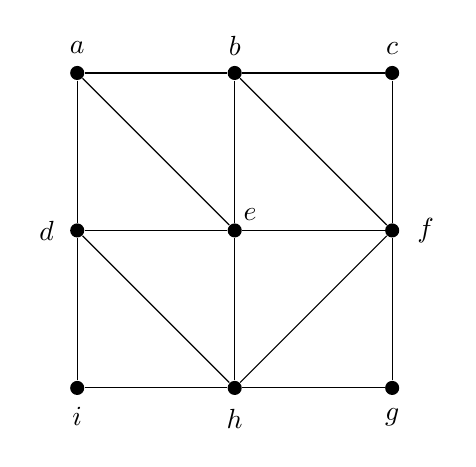
\begin{tikzpicture}[scale=2, every node/.style={circle, fill=black, inner sep=1.8pt}]
        
        % --- Define and Place Vertices (Grid Coordinates) ---
        % Top Row
        \node (a) at (0,2) {};
        \node (b) at (1,2) {};
        \node (c) at (2,2) {};
        
        % Middle Row
        \node (d) at (0,1) {};
        \node (e) at (1,1) {};
        \node (f) at (2,1) {};
        
        % Bottom Row
        \node (i) at (0,0) {};
        \node (h) at (1,0) {};
        \node (g) at (2,0) {};
        
        % --- Text Labels ---
        \node[fill=none, draw=none, above=3pt] at (a) {$a$};
        \node[fill=none, draw=none, above=3pt] at (b) {$b$};
        \node[fill=none, draw=none, above=3pt] at (c) {$c$};
        
        \node[fill=none, draw=none, left=4pt]  at (d) {$d$};
        \node[fill=none, draw=none, above right=2pt] at (e) {$e$};
        \node[fill=none, draw=none, right=4pt] at (f) {$f$};
        
        \node[fill=none, draw=none, below=4pt] at (i) {$i$};
        \node[fill=none, draw=none, below=4pt] at (h) {$h$};
        \node[fill=none, draw=none, below=4pt] at (g) {$g$};
        
        % --- Draw Grid Edges ---
        % Horizontal Edges
        \draw (a) -- (b) -- (c);
        \draw (d) -- (e) -- (f);
        \draw (i) -- (h) -- (g);
        
        % Vertical Edges
        \draw (a) -- (d) -- (i);
        \draw (b) -- (e) -- (h);
        \draw (c) -- (f) -- (g);
        
        % --- Draw Diagonal Edges ---
        \draw (a) -- (e);
        \draw (b) -- (f);
        \draw (d) -- (h);
        \draw (h) -- (f);
        
    \end{tikzpicture}

\end{center}

\mk{10} \yr{CSE 103 | L-1/T-2 | 2012--13}

%% 2013-14
\item Define Euler circuit and Hamiltonian circuit. State and prove the necessary and sufficient condition for the existence of an Euler circuit.
\mk{5+10} \yr{CSE 103 | L-1/T-2 | 2009--10}

%% 2012-13
\item For the complete bipartite graph $K_{n,m}$ where $n = 3$ and $m = 2$:
\begin{enumerate}
  \item Find an Euler path if it exists.
  \item Find a Hamiltonian circuit if it exists.
  \item What relationship must hold between $n$ and $m$ so that $K_{n,m}$ always has a Hamiltonian circuit?
\end{enumerate}
\begin{center}
      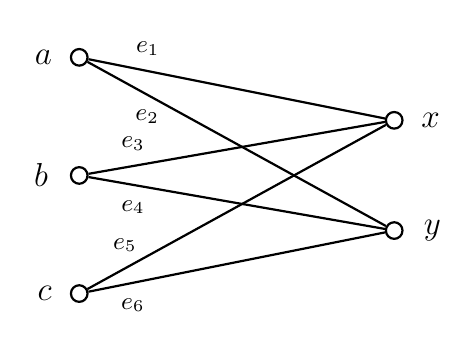
\begin{tikzpicture}[
        % ফাঁপা ও স্পষ্ট বৃত্তাকার নোডের স্টাইল
        every node/.style={circle, draw=black, fill=white, inner sep=0pt, minimum size=6pt, thick},
        line width=0.8pt,
        % এজের লেবেলগুলোর (e1, e2...) টেক্সট সাইজ এবং পজিশন স্টাইল
        edge label/.style={font=\small\itshape, draw=none, fill=none, inner sep=2pt}
    ]

        % --- বামপাশের নোডসমূহ (Left Set: a, b, c) ---
        \node (a) at (0, 3) {}; \node[draw=none, fill=none, anchor=east] at (-0.3, 3) {\large $a$};
        \node (b) at (0, 1.5) {}; \node[draw=none, fill=none, anchor=east] at (-0.3, 1.5) {\large $b$};
        \node (c) at (0, 0) {}; \node[draw=none, fill=none, anchor=east] at (-0.3, 0) {\large $c$};

        % --- ডানপাশের নোডসমূহ (Right Set: x, y) ---
        \node (x) at (4, 2.2) {}; \node[draw=none, fill=none, anchor=west] at (4.3, 2.2) {\large $x$};
        \node (y) at (4, 0.8) {}; \node[draw=none, fill=none, anchor=west] at (4.3, 0.8) {\large $y$};

        % --- এজসমূহ এবং তাদের নিখুঁত লেবেলিং (Edges & Labels) ---
        
        % নোড 'a' থেকে কানেকশন
        \draw (a) -- (x) node[pos=0.2, above, edge label] {$e_1$};
        \draw (a) -- (y) node[pos=0.2, below, edge label] {$e_2$};
        
        % নোড 'b' থেকে কানেকশন
        \draw (b) -- (x) node[pos=0.15, above, edge label] {$e_3$};
        \draw (b) -- (y) node[pos=0.15, below, edge label] {$e_4$};
        
        % நோড 'c' থেকে কানেকশন
        \draw (c) -- (x) node[pos=0.2, left, edge label, yshift=4pt] {$e_5$};
        \draw (c) -- (y) node[pos=0.15, below, edge label] {$e_6$};

    \end{tikzpicture}
\end{center}
\mk{9+9+9} \yr{CSE 103 | L-1/T-2 | 2008--09}

%% 2020-21
\end{enumerate}

%%──────────────────────────────────────────────────────────────────────
\subtopic{cE}{Graph Traversal}
\label{sub:s9-traversal}

\begin{enumerate}


%% 2023-24
\item The CSE department decides to make groups for tutorial classes for three courses: Machine Learning, Data Science, and Cybersecurity. Each group has 2 compulsory classes. Each class has 3 lesson plans. Each lesson has 2 practice tests.
For the binary search tree constructed from the names Obonti, Rahim, Mina, Ahmed, Shapla, Karim, Ezaz, Hasan, Lima, Bashir, determine the pre-order and post-order traversal.
\mk{5} \yr{CSE 103 | L-1/T-1 | 2023--24}

%% 2010-11
\item 

For the tree defined by the adjacency matrix:
\[
\begin{array}{c|ccccccc}
  & v_1 & v_2 & v_3 & v_4 & v_5 & v_6 & v_7 \\\hline
v_1 & 0 & 1 & 0 & 0 & 0 & 0 & 1 \\
v_2 & 1 & 0 & 1 & 1 & 0 & 0 & 0 \\
v_3 & 0 & 1 & 0 & 0 & 0 & 0 & 0 \\
v_4 & 0 & 1 & 0 & 0 & 1 & 0 & 1 \\
v_5 & 0 & 0 & 0 & 1 & 0 & 1 & 0 \\
v_6 & 0 & 0 & 0 & 0 & 1 & 0 & 0 \\
v_7 & 1 & 0 & 0 & 1 & 0 & 0 & 0 \\
\end{array}
\]
\begin{enumerate}
  \item Find the BFS tree.
  \item Find the DFS tree.
  \item Find the preorder traversal sequences.
  \item Find the postorder traversal sequence.
\end{enumerate}
\mk{3+3+3+3} \yr{CSE 103 | L-1/T-2 | 2010--11}


%% 2008-09
\item For a given binary tree, find the sequence of labels encountered when the tree is traversed in:
\begin{center}
      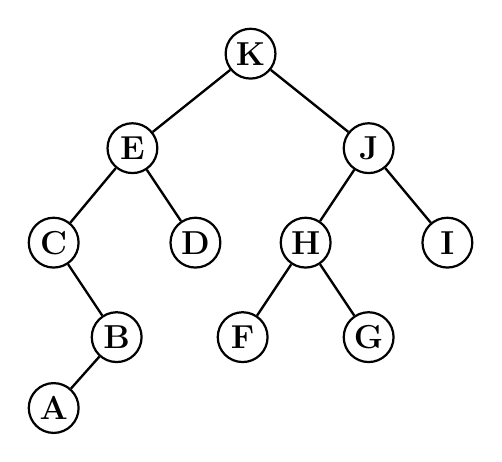
\begin{tikzpicture}[
        every node/.style={circle, draw=black, fill=white, inner sep=0pt, minimum size=18pt, font=\large\bfseries, thick},
        line width=0.85pt
    ]
        % --- লেভেল ০ ---
        \node (K) at (2.5, 4.5) {K};

        % --- লেভেল ১ ---
        \node (E) at (1.0, 3.3) {E};
        \node (J) at (4.0, 3.3) {J};

        % --- লেভেল ২ ---
        \node (C) at (0.0, 2.1) {C};
        \node (D) at (1.8, 2.1) {D};
        \node (H) at (3.2, 2.1) {H};
        \node (I) at (5.0, 2.1) {I};

        % --- লেভেল ৩ ---
        \node (B) at (0.8, 0.9) {B};
        \node (F) at (2.4, 0.9) {F};
        \node (G) at (4.0, 0.9) {G};

        % --- লেভেল ৪ ---
        \node (A) at (0.0, 0.0) {A};

        % --- এজ বা কানেকশনসমূহ (Connections) ---
        \draw (K) -- (E);
        \draw (K) -- (J);
        
        \draw (E) -- (C);
        \draw (E) -- (D);
        
        \draw (J) -- (H);
        \draw (J) -- (I);
        
        \draw (C) -- (B); % C থেকে ডানে হেলে B-তে গেছে
        \draw (B) -- (A); % B থেকে বামে হেলে A-তে গেছে
        
        \draw (H) -- (F);
        \draw (H) -- (G);

    \end{tikzpicture}
\end{center}

\begin{enumerate}
  \item Preorder
  \item Inorder
  \item Postorder
\end{enumerate}
\mk{9+9+9} \yr{CSE 103 | L-1/T-2 | 2008--09}

%% 2006-07
\item Consider a binary search tree.

\begin{center}
      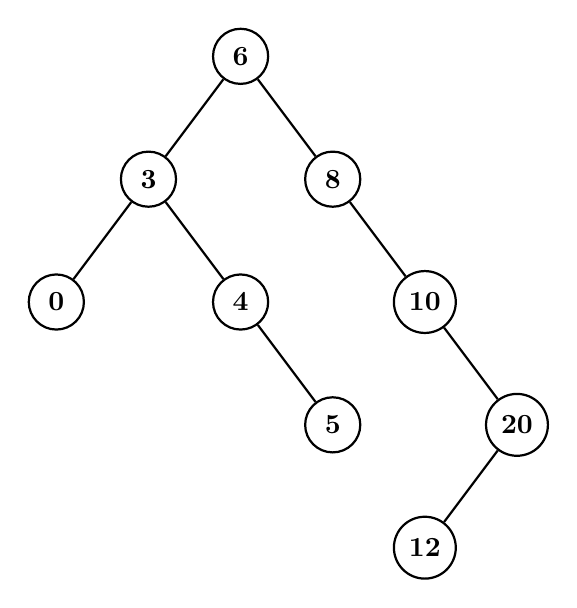
\begin{tikzpicture}[
        scale=1.3,
        % বৃত্তাকার নোডের জন্য সাধারণ স্টাইল
        every node/.style={circle, draw=black, thick, minimum size=0.7cm, font=\bfseries},
        thick,
        % লেভেল ডিস্ট্যান্স এবং সিবলিং ডিস্ট্যান্স সেট করা (ট্রি সুন্দর দেখানোর জন্য)
        level distance=1.2cm,
        sibling distance=1.8cm
    ]

        % --- Tree Structure ---
        \node {6}
            child {node {3}
                child {node {0}}
                child {node {4}
                    child[missing] % বাম চাইল্ড খালি রাখার জন্য
                    child {node {5}}
                }
            }
            child {node {8}
                child[missing] % বাম চাইল্ড খালি রাখার জন্য
                child {node {10}
                    child[missing] % বাম চাইল্ড খালি রাখার জন্য
                    child {node {20}
                        child {node {12}}
                        child[missing] % ডান চাইল্ড খালি রাখার জন্য
                    }
                }
            };

    \end{tikzpicture}
\end{center}

Which order of tree traversal will print the elements in ascending order? Why?
\mk{4} \yr{CSE 103 | L-1/T-2 | 2006--07}

\end{enumerate}

%%──────────────────────────────────────────────────────────────────────
\subtopic{cE}{Trees}
\label{sub:s9-trees}

\begin{enumerate}

%% Session: 2024-2025
\item (i) In a college, Amrin is friend of Badal, Mina, Harish and Elina. Mina has friendship with Badal, Elina and Dulal. Dulal has friendship with Badal, Elina and Mina too (already has been mentioned), and he has two more friends Irin and Farid. Irin and Farid each of them is a friend of Harish. Harish and Farid have a common friend Galib. Badal is a friend of Irin too and it has been already mentioned that Harish and Amrin are friends. During student union election, who are friends, can not be profile checker as they can be biased. Identify who can check whose profile.
\mk{12} \\
%% Session: 2024-2025
(ii) If the college authority wants to analyze the friendship tree such a way that friend of friends will be listed first, find the tree from the above friend circle. Here, the college authority decided to start with Dulal.
\mk{5} \yr{CSE 103 | L-1/T-I | 2024--25}

%% Session: 2024-2025
\item Mrs. Sazida, a math teacher wants to teach frequency to the kids by writing a character sequence like this: cccc hhh IIIIII tttttttttt aaaaa gg o nnnnnnnnn (ignore space), where different letters appear with different frequencies. Design a search tree based on the frequency of the character so that the character with higher frequency appears at the one side of the node, and the character of lower frequency appears on the other side of the node.
\mk{8} \yr{CSE 103 | L-1/T-I | 2024--25}

%% 2015-16
\item The CSE department decides to make groups for tutorial classes for three courses: Machine Learning, Data Science, and Cybersecurity. Each group has 2 compulsory classes. Each class has 3 lesson plans. Each lesson has 2 practice tests.
\begin{enumerate}
  \item Find the hierarchical organization of the tutorial program (draw the tree).
  \item Find the organization indexed with an array.
  \item Design a binary search tree with the given order of names: Obonti, Rahim, Mina, Ahmed, Shapla, Karim, Ezaz, Hasan, Lima, Bashir, and Tapan.
\end{enumerate}
\mk{20} \yr{CSE 103 | L-1/T-1 | 2023--24}
%% 2022-23
\item Represent an organization's organogram with a suitable graph where it is led by the president Rahima Sultana, who leads 3 vice presidents. Each vice president leads 2 directors. Each director leads 3 team leaders, and each team has 4 members.
\begin{enumerate}
  \item Draw the organogram tree. If the president wants to broadcast a message, determine the number of levels she needs to pass.
  \item What will be the adjacency list to represent this organogram?
\end{enumerate}
\mk{5+1+4} \yr{CSE 103 | L-1/T-1 | 2022--23}

%% Session: 2021-2022
\item 'Tomorrow will be a day off'. Prof Sharifa Sultana sends email to the Class Representatives (CRs) CR4A, CR4B, CR4C of three sections of Level 4 respectively. CR4A will send emails to CR's of Level 3- CR3A, CR3B, CR3C. CR4B will send emails to CRs of Level 2, and CR4C will send emails to CRs of Level 1. Each level has three sections. Represent the scenario with a suitable graph. What will be the number of edges and vertices in the graph? What will be the total number of the emails? (Show the breakdown of the computation).
\mk{10} \yr{CSE 103 | L-1/T-I | 2021--22}

%% 2006-07
\item Prove the following properties of a tree:
\begin{enumerate}
  \item There is a unique simple path between every pair of vertices in a tree.
  \item Adding an edge between two vertices in a tree creates a cycle.
  \item Removing any edge from a tree disconnects the graph.
  \item In a tree with at least two vertices, there are at least two leaves.
  \item The number of vertices is one larger than the number of edges.
\end{enumerate}
\mk{15} \yr{CSE 103 | L-1/T-2 | 2020--21}

%% Jan 2021 — BST with scores
\item Instructor Rafiq Ahmed stores the scores of his students in the form of a Binary Search Tree. The scores are: 76, 55, 90, 38, 45, 83, 100, 93, 86. Find the Binary Search Tree. Find the internal nodes and the height of the tree. Write down the pre-order traversal if your student ID is odd, or the post-order traversal if your student ID is even. (Example: a student with ID 2105001 traverses in pre-order.)
\mk{12} \yr{CSE 103 | L-1/T-2 | Jan 2021}

%% 2008-09
\item The expression $((2+3) * (7 - 6*(8/4) + 3)) * 2 * (18/3)$ is given in infix form. Build the binary expression tree from this infix expression. (For example, for $2+3$, `$+$' will be the root, 2 will be the left child, and 3 will be the right child.)
\mk{4} \yr{CSE 103 | L-1/T-2 | Jan 2020}

%% Jan 2020
\item After building the expression tree for $((2+3)*(7-6*(8/4)+3))*2*(18/3)$:
\begin{enumerate}
  \item Find the postorder traversal of the tree and the height of the tree.
  \item For a complete 3-ary tree, what will be the total number of nodes for height 3?
\end{enumerate}
\mk{4+4} \yr{CSE 103 | L-1/T-2 | Jan 2020}

%% 2011-12
\item Given symbols with frequencies A(4), B(3), C(1), D(1), E(15), F(2), G(5), H(4), construct a Huffman tree so that sending codes of variable length requires the minimum number of bits. Show the total number of bits required.
\mk{10} \yr{CSE 103 | L-1/T-2 | 2017--18}  


%% Jan 2020
\item Prove that the height of a full and balanced $m$-ary tree with $l$ leaves is $h = \lceil \log_m l \rceil$.
\mk{15} \yr{CSE 103 | L-1/T-2 | 2016--17}

%% 2017-18
\item Define the following with respect to rooted trees: (i) ancestor, (ii) leaf, (iii) level, (iv) height.
\mk{8} \yr{CSE 103 | L-1/T-2 | 2015--16}

%% 2015-16
\item Define the following, and give one example of each type of tree of height 4:
\begin{enumerate}
  \item Full $m$-ary tree.
  \item Balanced $m$-ary tree.
  \item Complete $m$-ary tree.
\end{enumerate}
\mk{9} \yr{CSE 103 | L-1/T-2 | 2015--16}

%% 2015-16
\item How many vertices does a full 5-ary tree with 100 internal vertices have?
\mk{5} \yr{CSE 103 | L-1/T-2 | 2015--16}

%% 2016-17
\item Find the minimum cost spanning tree if you start from vertex $a$, using Kruskal's algorithm. Show all steps.
\begin{center}
  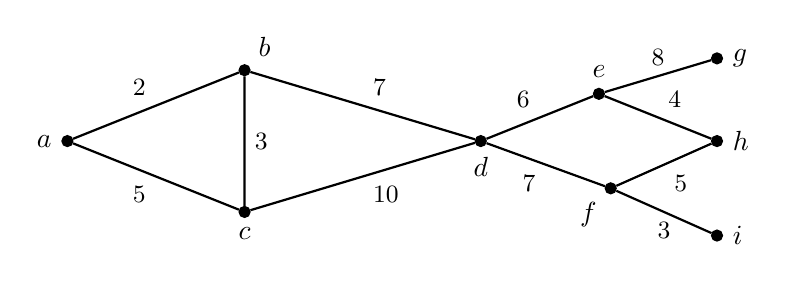
\begin{tikzpicture}[
    scale=1.5,
    vertex/.style={circle, draw, fill=black, inner sep=0pt, minimum size=4pt},
    edge_label/.style={font=\small}
]

    % ==========================================
    % VERTICES (Positions based on the sketch)
    % ==========================================
    \node[vertex, label=left:{$a$}] (a) at (0,0) {};
    \node[vertex, label=above right:{$b$}] (b) at (1.5,0.6) {};
    \node[vertex, label=below:{$c$}] (c) at (1.5,-0.6) {};
    \node[vertex, label=below:{$d$}] (d) at (3.5,0) {};
    \node[vertex, label=above:{$e$}] (e) at (4.5,0.4) {};
    \node[vertex, label=below left:{$f$}] (f) at (4.6,-0.4) {};
    \node[vertex, label=right:{$g$}] (g) at (5.5,0.7) {};
    \node[vertex, label=right:{$h$}] (h) at (5.5,0) {};
    \node[vertex, label=right:{$i$}] (i) at (5.5,-0.8) {};

    % ==========================================
    % EDGES AND WEIGHTS
    % ==========================================
    % Left diamond block
    \draw[thick] (a) -- (b) node[midway, above left, edge_label] {2};
    \draw[thick] (a) -- (c) node[midway, below left, edge_label] {5};
    \draw[thick] (b) -- (c) node[midway, right, edge_label] {3};
    \draw[thick] (b) -- (d) node[midway, above right, edge_label] {7};
    \draw[thick] (c) -- (d) node[midway, below right, edge_label] {10};

    % Right branch structures
    \draw[thick] (d) -- (e) node[midway, above left, edge_label] {6};
    \draw[thick] (d) -- (f) node[midway, below left, edge_label] {7};
    
    \draw[thick] (e) -- (g) node[midway, above, edge_label] {8};
    \draw[thick] (e) -- (h) node[midway, above right, edge_label] {4};
    
    \draw[thick] (f) -- (h) node[midway, below right, edge_label] {5};
    \draw[thick] (f) -- (i) node[midway, below, edge_label] {3};

\end{tikzpicture}
\end{center}

\mk{13} \yr{CSE 103 | L-1/T-2 | 2013--14}

%% 2013-14
\item Find the game tree for the next player's turn in the given Tic-tac-toe grid. Player 1 starts first with `X'.
\begin{center}
  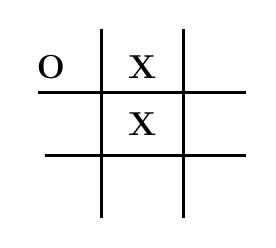
\begin{tikzpicture}[scale=0.8, line width=1.2pt]

    % ==========================================
    % GRID LINES
    % ==========================================
    % Vertical lines
    \draw (1, -1.5) -- (1, 1.5);
    \draw (2.3, -1.5) -- (2.3, 1.5);
    
    % Horizontal lines
    \draw (0, 0.5) -- (3.3, 0.5);
    \draw (0.1, -0.5) -- (3.3, -0.5);

    % ==========================================
    % GAME MARKS (O and Xs)
    % ==========================================
    % 'O' in the top-left corner (positioned slightly above the line like the sketch)
    \node[font=\large\bfseries] at (0.2, 0.9) {O};
    
    % 'X' in the top-middle cell
    \node[font=\large\bfseries] at (1.65, 0.9) {X};
    
    % 'X' in the center cell
    \node[font=\large\bfseries] at (1.65, 0.0) {X};

\end{tikzpicture}
\end{center}

\mk{13} \yr{CSE 103 | L-1/T-2 | 2013--14}  

%% 2023-24
\item Prove that there are at most $m^h$ leaves in an $m$-ary tree of height $h$.
\mk{10} \yr{CSE 103 | L-1/T-2 | 2011--12}

%% 2011-12
\item How can you search for items in a list efficiently using trees? Describe with an example.
\mk{6} \yr{CSE 103 | L-1/T-2 | 2011--12}

%% 2013-14
\item A saturated hydrocarbon molecule is modelled as a tree $T$, where each carbon atom is an internal vertex and each hydrogen atom is a degree-one vertex (leaf). Prove that $k = 2n + 2$, where $k$ is the number of hydrogen atoms and $n$ is the number of carbon atoms.
\begin{center}
    % The \chemfig command draws the molecule node by node
    \chemfig{
        C(-[:180]H)(-[:135]H)(-[:225]H) % Leftmost Carbon with 3 H's
        - C(-[:135]H)(-[:225]H)         % Middle Carbon with 2 H's
        - C(-[:0]H)(-[:-90]H)           % Rightmost horizontal Carbon with 2 H's
        -[:90] C(-[:180]H)(-[:0]H)-[:90]H % Top Carbon with 3 H's
    }
    
    \vspace{1.5em}
    ``A saturated hydrocarbon tree T''
\end{center}

\mk{8} \yr{CSE 103 | L-1/T-2 | 2010--11}

%% 2010-11
\item Define ``height'', ``leaf'', and ``level'' of a tree. Find the height and leaf nodes of a tree represented by the following $7 \times 7$ adjacency matrix (where $v_2$ is the root):
\[
\begin{array}{c|ccccccc}
  & v_1 & v_2 & v_3 & v_4 & v_5 & v_6 & v_7 \\\hline
v_1 & 0 & 1 & 0 & 0 & 0 & 0 & 1 \\
v_2 & 1 & 0 & 1 & 1 & 0 & 0 & 0 \\
v_3 & 0 & 1 & 0 & 0 & 0 & 0 & 0 \\
v_4 & 0 & 1 & 0 & 0 & 1 & 0 & 1 \\
v_5 & 0 & 0 & 0 & 1 & 0 & 1 & 0 \\
v_6 & 0 & 0 & 0 & 0 & 1 & 0 & 0 \\
v_7 & 1 & 0 & 0 & 1 & 0 & 0 & 0 \\
\end{array}
\]
\mk{7} \yr{CSE 103 | L-1/T-2 | 2010--11}

%% 2010-11
\item Draw the Huffman tree for the letters z, a, e, i, o, and y with frequencies 4, 7, 12, 17, 20, and 28 respectively. What will be the encoding for the word ``eye''?
\mk{8} \yr{CSE 103 | L-1/T-2 | 2010--11}

\item Prove that if $T$ is a binary tree of height $h$ and with $n$ nodes, then
\[
  h + 1 \leq n \leq 2^{h+1} - 1.
\]
\mk{10} \yr{CSE 103 | L-1/T-2 | 2008--09}

%% 2010-11
\item Show that the number of leaves on a complete binary tree is always one greater than the number of interior nodes of the tree.
\mk{7} \yr{CSE 103 | L-1/T-2 | 2006--07}

%% 2006-07
\item Find an expression for the number of leaves on a complete $n$-ary tree in terms of the number of interior nodes of the tree.
\mk{8} \yr{CSE 103 | L-1/T-2 | 2006--07}

%% 2006-07
\item Represent the following propositional form as an ordered binary tree:
\[
  \bigl[(A \lor B) \implies C\bigr] \iff (D \lor A).
\]
\mk{5} \yr{CSE 103 | L-1/T-2 | 2006--07}

%% 2006-07
\item Give an example of two trees representing two different mathematical expressions but producing the same word when in-order traversal is used.
\mk{6} \yr{CSE 103 | L-1/T-2 | 2006--07}



%% 2020-21 — Tree properties
\end{enumerate}



\end{document}